\documentclass{article}
\usepackage{import}
\usepackage[utf8]{inputenc}
\usepackage{amsmath}
\usepackage{amssymb}
\usepackage{mathtools}
\usepackage{graphicx}
\usepackage{tabularx}
\usepackage{float}
\usepackage{subfig}
\usepackage{lscape} 
\usepackage{hyperref}
\usepackage{setspace}
\usepackage{booktabs}
\usepackage[authoryear]{natbib}
\usepackage{lmodern}
\usepackage[T1]{fontenc}
\usepackage[bottom]{footmisc}
\newcommand{\indep}{\perp \!\!\! \perp}
\usepackage[nolist]{acronym}
\newcommand\headercell[1]{%
   \smash[b]{\begin{tabular}[t]{@{}c@{}} #1 \end{tabular}}}
\usepackage[a4paper,top=3cm,bottom=2cm,left=3cm,right=3cm,marginparwidth=1.75cm]{geometry}
\usepackage{xcolor}%
\definecolor{webbrown}{rgb}{.6,0,0}
\usepackage{hyperref}%
\hypersetup{%
  breaklinks = true,%
  colorlinks = true,%
  anchorcolor = webbrown,%
  citecolor = webbrown,%
  filecolor = webbrown,%
  linkcolor = webbrown,%
  menucolor = webbrown,%
  urlcolor= webbrown,%
  citebordercolor= 1 0 0,%
  menubordercolor=1 0 0,%
  urlbordercolor=1 0 0,%
  runbordercolor=1 0 0,}
\usepackage{cleveref}

\usepackage{setspace}
\usepackage{enumitem}
\setstretch{1.5} %% set line spacing

\begin{acronym}
  \acro{CI}{confidence interval}
  \acro{RCT}{randomized controlled trial}
  \acro{IV}{instrumental variable}
  \acro{LATE}{local average treatment effect}
  \acro{ATE}{average treatment effect}
  \acro{OLS}{ordinary least squares}
  \acro{RD}{regression discontinuity}
  \acro{MTE}{marginal treatment effect}
  \acro{ATT}{average treatment effect on the treated}
\end{acronym}

\graphicspath{ {../../output/figures/} }

% Wrap table notes
\usepackage{booktabs}
\newcommand{\tabnotes}[2]{\bottomrule \multicolumn{#1}{@{}p{0.70\linewidth}@{}}{\footnotesize #2 }\end{tabular}\end{table}}

\floatplacement{figure}{H}
\floatplacement{table}{H}

\usepackage[toc,page]{appendix}


\title{Arrest Rates and College Enrollment:
\texorpdfstring{\\}{} Examining the Impact of Two Federal Drug Control Acts}
\author{Ray Huang\thanks{Contact:
    \href{mailto:ray_huang@brown.edu}{ray\_huang@brown.edu}.
     I am grateful to Peter Hull at Brown University for serving as my advisor and for providing me with fantastic feedback and guidance. I would also like to thank Alison Lodermeier and Francesco Ferlenga for their generous comments and support. A replication archive is available at https://github.com/rayhuang11/EconSeniorThesisRH.}
     \\Brown University, Honors Thesis}

\date{\today}

\begin{document}

\maketitle

\begin{abstract}
\noindent I examine the impact of two federal drug acts on college enrollments and earnings among Black males by using a variety of counterfactual groups. The Anti-Drug Act of 1986 transformed the formerly rehabilitation-focused justice system into a punitive one, imposed sentencing minimums and disparities. The Fair Sentencing Act of 2010 was intended to reverse some of these policies. I construct estimates of the impact of these two acts on the college enrollment of Black males aged 18-24 using three distinct counterfactual groups: 1) comparing states with high drug arrests to states with low drug arrests, 2) Black males to White males, and 3) Black males to Black females. I also evaluate the first stage impact of the two Acts on drug-related arrests. I find that

\end{abstract}

\clearpage

\section{Introduction}
 
% Motivation

\begin{quote}
  There’s 2.2 million people in the American prison system, and half a million of those are locked up for drug offenses. A lot of them were in the same boat as me: victims of the mandatory minimum. Passed by Congress in 1986, it’s the reason hundreds of thousands of nonviolent people, mostly black and brown people, are rotting in prison... I’d been in prison for ten years by the time my petition reached the Supreme Court. (HONY Interview)
\end{quote}

College enrollment rates provide insights into several aspects of the educational landscape, such as access to higher education, socioeconomic factors, and workforce development. In the decades following 1970, the rate of college enrollment growth for black males began to fall behind all other groups, including white females and black females. Simultaneously, incarceration rates for black males began to climb during this period, as demonstrated in figure \ref{fig:raw_ab}. Many blame the Anti-Drug Abuse Act of 1986 for the increase in minority incarcerations. In 2010, the Fair Sentencing Act was passed, which aimed to undo many of the racial disparities potentially caused by the Anti-Drug Abuse Act. In this paper, I look to investigate the link between drug enforcement policies and educational outcomes, as I examine the impact of the Anti-Drug Abuse Act of 1986 and Fair Sentencing Act of 2010 on both drug-related arrest rates and college enrollment among Black males.

% This paper

This paper has two main objectives. First, I look to estimate the impact of the Anti-Drug Abuse Act of 1986 and the Fair Sentencing Act of 2010 on drug-related arrests. The second objective is to evaluate the impact of the two acts on college enrollment rates for Black males. Additionally, I examine the relationship between drug-related arrest rates and college enrollment. 

% Methods

I use three separate research designs. The first and primary research design combats the endogeneity problem by leveraging variations in the intensity of drug arrests across different states. High-intensity states are defined as states with Black adult drug-related arrest rates above the 75th percentile two years before the passage of the federal drug act (e.g. for the Anti-Drug Abuse Act, 1984 was used.) I compare high-intensity states to low-intensity states, and I calculate both the first stage and reduced form estimates where the first stage is the impact of the act on Black adult drug-related arrest rates and the reduced form is the impact of the act on college enrollment. For additional supplemental analysis, I adapt the second and third research designs in \cite{britton2022} to estimate the impact of the federal drug acts on college enrollment at the individual level.

% Data

I use repeated cross-sectional data from the Current Population Survey October education supplement for data at the individual level, and I limit my analysis to persons aged 18-24 at the time of the passage of the act. For data on arrests, I use data from the Uniform Crime Reporting Program, which contains information on the number of arrests by race, crime type, and juvenile crimes. To construct college enrollment rates from the CPS, I count any individual who is currently in their first year or has more than one year of college education \footnote{I count individuals with a master's or Ph.D. as having been enrolled in college. I also count persons enrolled in two-year colleges.}.

This data has several limitations. First, the CPS excludes currently incarcerated populations. Second, the UCR has well-documented quality issues, such as many counties failing to report in certain years. In certain years, entire states failed to report any arrest data. Overall, if the effect size is small, the data might be insufficiently powered.

% Findings

I find that the Anti-Drug Abuse Act of 1986 had a modest impact on Black adult male arrest rates and a small negative impact on college enrollment. In addition, I find some evidence that an increase in Black adult drug-related arrest rates has a small negative impact on college enrollment rates. The Fair Sentencing Act of 2010 is harder to study due to substantial pretrends, and I find some evidence of a potentially positive impact on college enrollment for Black males. For my estimates to be considered causal, important pretrend and exclusion restrictions must be satisfied.

% Literature
This paper heavily builds upon recent work by \cite{britton2022}, who estimates the impact of the Anti-Drug Abuse Act on college enrollment and the impact of state-level legislation on college enrollment. She finds that "Black males had a 2.2 percentage point decrease in the relative probability of college enrollment after the passage of the Anti-Drug Abuse Act of 1986." I build upon her work by introducing a new counterfactual group that allows the impact to be split into a first-stage and reduced-form. I also introduce more modern and robust methods to deal with the issue of pretrends, and I spend some time replicating her results.

This paper generally contributes to the literature on the effects of incarceration on education and labor outcomes. My main contribution to the literature is a relatively imprecise and subpopulation-specific estimate of the causal effect of an increase in Black adult drug-related arrest rates on college enrollment.

Some related prior literature includes \cite{aizer} which evaluates the relationship between juvenile incarceration and later life outcomes using a judge-IV research design. They find that juvenile incarceration "results in large decreases in the likelihood of high school completion and large increases in the likelihood of adult incarceration." \cite{western} evaluates the impact of incarceration on labor market outcomes. \cite{mitchell2016effect} finds that changes in drug arrest rates did not reduce the rate of drug offenses but had substantial negative impacts on employment outcomes for Black males. \cite{hatzenbuehler2015collateral} finds that high incarceration rates have psychiatric impacts on non-incarcerated populations, implying that if the federal drug acts have a large impact on arrest rates, there may be spillover effects.

The rest of the paper is organized as such: in section 2 I summarize the history and known impacts of the Anti-Drug Abuse Act and Fair Sentencing Act. In section 3 I describe my empirical strategies, and in section 4 I discuss the data and its flaws. I present my results in section 5, and I close in section 6 with conclusions and implications.

\section{Background}

The Anti-Drug Abuse Act of \citeyear{antidrugabuseact1986} was passed in October of 1986 as part of Reagan's War on Drugs in response to the growing concerns over drug abuse, particularly the crack cocaine epidemic. The Anti-Drug Abuse Act of 1986 marked a pivotal shift in the nation's approach to drug policy, emphasizing punitive measures and significantly impacting the criminal justice system. Several notable changes in drug policy were introduced, including the establishment of mandatory minimum sentences for drug offenses. One of the most controversial aspects of the legislation was the implementation of the 100-to-1 sentencing disparity between crack and powder cocaine offenses. This disparity mandated that possession of 5 grams of crack cocaine resulted in a minimum 5-year prison sentence, while it took 500 grams of powder cocaine to trigger the same penalty. Critics argued that this disparity disproportionately affected minority and low-income communities, as crack cocaine was more prevalent in these populations. The \cite{eji} claims that after the act, the number of Black people in federal prison increased from 50 in 100,000 to 250 in 100,000, yet there was no change in the number of White people in federal prison \footnote{The Equal Justice Initiative did not include their source, and I could not find any other source making the same claim.}. The act also allocated substantial funds for drug enforcement, treatment, and prevention programs, reflecting the government's commitment to addressing the drug crisis comprehensively. The \cite{drug_control_money} estimated that drug control funding increased from \$2.9 billion in 1986 to \$4.8 billion in 1987. The Act has faced additional criticism as in recent years researchers such as \cite{bewley2005incarceration} have found that "there is little correlation between incarceration rates and drug use prevalence; and the impact of enforcement action on price is much less powerful than other market factors."

It is important to note that due to the War on Drugs, arrest rates and sentencing times were trending up even before the Anti-Drug Abuse Act of 1986. \cite{bjs_1986} reported that from 1980 to 1986, the number of federal drug law violations that resulted in convictions increased by 134\% to a total of 12,285 convictions in 1986 \footnote{Federal convictions of all other types increased by 27\%.}. The BJS report also notes that average prison sentences for drug offenders increased by 33\% less than four years to over five years.

The Fair Sentencing Act of 2010 was a piece of legislation enacted by the United States Congress to address the sentencing disparities between crack and powder cocaine offenses, which had been established by the Anti-Drug Abuse Act of 1986. The 2010 act aimed to reduce the disproportionate impact of drug laws on minority and low-income communities by amending the previously imposed 100-to-1 sentencing disparity. Under the new legislation, the ratio was reduced to 18-to-1, meaning that it now took 28 grams of crack cocaine to trigger a mandatory minimum sentence of 5 years, instead of the previous 5 grams, while the threshold for powder cocaine remained at 500 grams. Furthermore, the Fair Sentencing Act eliminated the mandatory minimum sentence for simple possession of crack cocaine, emphasizing a more equitable approach to drug offenses. Though the act did not completely equalize the sentencing for crack and powder cocaine, it represented a significant step toward a fairer criminal justice system and demonstrated the government's commitment to addressing the consequences of previous drug policies. A \cite{ussc} report estimated that implementing the Fair Sentencing Act of 2010 resulted in the saving of 29,653 bed years \footnote{The same \cite{ussc} report also found that the Fair Sentencing Act of 2010 did not "disrupt the ongoing decline in the number of people who reported using crack cocaine in the last year."}. 


\section{Empirical Strategy}

I take three discrete approaches to my empirical strategy, establishing three unique counterfactual groups for identifying the impact of the Anti-Drug Abuse Act of 1986 and the Fair Sentencing Act of 2010 on college enrollment rates. 

My first and primary empirical approach looks at changes in college enrollment rates in high drug arrest states relative to the low drug arrest states before and after the passage of both the 1986 and 2010 acts where high drug arrest states are defined as states above the 75th percentile two years before the passage of the federal law \footnote{For the Anti-Drug Abuse Act of 1986, states with high Black adult normalized arrest rates include CT, DC, GA, IL, MD, MA, MO, NJ, NY, and TN. States with high Black juvenile normalized arrest rates include AR, CT, DE, DC, ME, MD, MA, MT, NJ, SD, and TN. For the Fair Sentencing Act of 2010, states with high Black adult normalized arrest rates include AL, AR, DE, DC, GA, KY, LA, MD, MS, MO, NJ, NC, TN, and VA. States with high Black juvenile normalized arrest rates include AL, DE, DC, GA, IL, KY, LA, MD, MS, MO, NJ, NC, PA, and SC. Note that states without any UCR Program drug arrest data are omitted from this analysis. See figure \ref{fig:heatmap} for a heatmap of high-intensity states in 1984.}. I primarily rely on data on adult arrests instead of juvenile arrests due to effect sizes and issues with pretrends \footnote{As discussed in the introduction, \cite{aizer} finds that juvenile incarceration has a larger impact on education than adult incarceration. However, since states with high adult arrests tend to have high juvenile arrest rates, my estimates are robust to which arrest rate is used.}. I examine the first-stage impact where the outcome is the change in drug-related arrest rates and the reduced-form impact where the outcome is college-enrollment. The first stage is evaluated using an event-study model that allows me to assess the evolution of relative outcomes while controlling for fixed differences across states and national trends over time. Using data at the state ($s$) by year ($t$) level, I estimate:

\begin{equation} \label{eq:state_level_es}
  y_{st} = \alpha_s + \gamma_t + X'_{st} \phi + \sum_{m=-G}^{M} \beta_m z_{s,t-m} + \epsilon_{st}
\end{equation}

where $\alpha_s$ and $\gamma_t$ are individual and time fixed effects, $X'_{st}$ is a vector of control variables, and $\epsilon_{st}$ represents a shock uncorrelated with the policy. The coefficients $\{\beta_m \}^{M}_{m=-G}$ summarize the magnitude of the dynamic effects and are displayed in an event-study plot \footnote{Since the Anti-Drug Abuse Act was passed in October, I normalize the $\beta$ in 1986 to be zero. Similarly, since the Fair Sentencing Act of 2010 was passed in August, I normalize the $\beta$ on 2010 to be zero.}. When testing for pre-trends, if the first-stage arrest rates are trending similarly before the passage of the Anti-Drug Abuse Act of 1986 and the Fair Sentencing Act of 2010, I expect the coefficients associated with pre-periods to be small and statistically insignificant.

For the reduced form estimates, I follow a similar approach where use an event-study model identical to the model specified in \ref{eq:state_level_es}, except I replace ($s$) with($i$), as data is at the individual by year level. In addition to the event study analyses, I also report traditional difference-in-differences estimates as a summary of the effect across all post-expansion years using the following regression specification at the individual ($i$) by year ($t$) level: 

\begin{equation} \label{eq:did}
  y_{it} = \alpha + \zeta_s + \xi_t + \delta D_i + \gamma Post_t + \beta D_i Post_t + X'_{it}\phi + \epsilon_{it}
\end{equation}

where $\zeta_s$ and $\xi_t$ are fixed effects at the state and year level, $D_{i}$ is an indicator for belonging to the treatment group (in this case, states with high drug arrests), $Post_t$ is a time indicator for belonging to the post-period, $D_i Post_t$ is the interaction term where $\beta$ is potentially the causal effect of the federal policy if the identifying assumptions are satisfied, and $X'_{it}$ is a vector of control variables. For the reduced form estimates, I report three specifications of the difference-in-difference estimates: the first omits control variables and fixed effects, the second omits fixed effects, and the third is the full regression as specified in \ref{eq:did}. To increase power, I also include difference-in-difference regressions with a continuous treatment variable instead of an indicator variable.

To address issues of low power associated with event study tests for pre-trends in both the first stage and reduced form regressions, I implemented suggestions from \cite{roth2022}, which include calculating the slope of a linear violation of parallel trends that a pre-trends test would detect a specified fraction of the time, the expected value of the coefficients conditional on passing the pre-test under the hypothesized trend, and useful statistics such as power, Bayes Factor, and likelihood ratio.

Overall, examining both the first-stage and reduced-form impact of the federal has the advantage of enabling me to estimate the impact of arrest rates on college enrollment for Black males. I conduct an instrumented difference-in-differences (DDIV) estimate where the endogenous variable is arrest rates and the instrument is an indicator for living in a high-intensity state. I follow the advice given in \cite{ddiv}. For my DDIV estimates to be causal, the exclusion restriction must be satisfied, i.e. it must be the case that college enrollment is only impacted through changes in arrest rates.  I report the DDIV estimator as the simple ratio of means, and I also calculate the DDIV estimator via two-stage least squares (2SLS). If the exclusion restriction is satisfied, then my estimate applies to populations whose arrest rate was increased by the federal drug act. To check whether my estimates may be affected by the weak-instrument problem, I report F-statistics.

My second and third empirical strategies mirror the approach taken in \cite {britton2022}. In my second empirical strategy, I compare changes in college enrollment rates in Black males aged 18-24 relative to white males aged 18-24 at the time of the federal law passage. My third approach is very similar to the second approach, where I look at the change in college enrollment rates in Black males aged 18-24 at the time of the federal law passage relative to female Blacks aged 18-24 at the time of the federal law passage. I report traditional difference-in-difference estimates using the regression specified in \ref{eq:did}, except in the second empirical approach $D_i$ is an indicator for being Black (while the entire sample is limited to Black and White males), and in the third empirical approach $D_i$ is an indicator for being a Black male (while the entire sample is limited to Blacks aged 18-24 at the time of the federal law passage.).

Finally, I also include a triple difference-differences specification, where the first difference is pre and post-time periods, the second difference is race, and the third difference is living in a high or low-Black drug arrest state. The identifying assumption for the triple difference is 

To test whether the identifying assumptions for the three counterfactual groups were satisfied, aside from including event-study plots, I included plots of the raw outcomes over time.

In all the regression specifications, I estimate the equation using ordinary least squares (OLS). I also follow the recommendations outlined in \cite{duflo_did} and report heteroskedasticity-robust standard errors that are clustered at the state level. All analyses use CPS October supplement final person weights and limit the sample to Black males aged 18-24 at the time of the passage of the federal act.

\section{Data and Descriptive Statistics}

\subsection{Data}
% CPS
To conduct my analysis, I use data from three sources. My primary data source is the Current Population Survey (CPS) October Education Supplement from 1980-2016, which I accessed via the IPUMS-CPS database \citep{ipums_cps} \footnote{Following \cite{britton2022}, for most of my analysis of the Anti-Drug Abuse Act of 1986, I only use years from 1984 onwards. Further discussion of this point is included in the appendix.}. The Current Population Survey Education Supplement (CPS) is an annual cross-sectional survey conducted by the United States Census Bureau and the Bureau of Labor Statistics, collecting data from a nationally representative sample of approximately 60,000 households. Focused on educational attainment, enrollment status, and related socio-economic factors, the CPS provides a snapshot of the U.S. population's educational landscape, which is instrumental in shaping educational policies and understanding trends, and the CPS is commonly used in the social sciences. Following the approach in \cite{britton2022}, I excluded observations missing relevant data such as family income and educational attainment, which reduced the sample by about five percent. I defined college enrollment to be persons who had 1 year or more of higher education, and I limited my analysis to persons aged 18-24 in the year the federal law was passed (1986 and 2010). One notable limitation of the CPS is that it excludes the currently incarcerated population, which would result in an underestimate of the impact of both the Anti-Drug Abuse Act of 1986 and the Fair Sentencing Act of 2010. The CPS also does not account for movement across state lines.

%UCR
For data on arrests, I used the Uniform Crime Reporting (UCR) Program Data from the \cite{ucr}. The UCR Program is a data collection initiative led by the FBI, which amasses crime statistics from local law enforcement agencies throughout the United States, and the UCR data is commonly used for crime-related social science research topics. The UCR Program has data at the county-year level and includes information on the number of arrests for each arrest type (e.g. drug possession, drug distribution, assault, robbery, etc) and also records data on the age \footnote{The UCR data separately tracks arrest rates for adult and juvenile cases.} and race of the arrested. In my analysis, I use Black adult arrests and Black juvenile arrests related to all drug crimes \footnote{The universe of all drug crimes corresponds to code 18 in the UCR program data. The UCR program includes data on drug offenses at a more granular level, such as type of drug, weight, and sale to a minor.}. Since I needed arrest data at the state and year level, I constructed a normalized arrest rate per 100,000 by averaging the arrest rate for counties with available data in a state together and dividing by the state's population in the given year \footnote{The population in each state-year was taken from the CPS.}. In any analysis where I used both UCR and CPS data, I merged the two datasets at the state and year level \footnote{The merged dataset is henceforth referenced as CPS-UCR merged dataset}.

It is important to note that the UCR data has several limitations. First and foremost, many counties failed to report their arrest rates for certain years. Secondly, the UCR's hierarchical reporting system requires that only the most severe crime be recorded in cases of multiple offenses, which may skew the data. Finally, variations in reporting practices among different law enforcement agencies, as well as changes in reporting standards over time, can affect the consistency and comparability of the data. Notably, in my sample, in certain years, one state failed to report any arrest data, which resulted in all persons living in said state being dropped from the analysis \footnote{Approximately 10,000 observations per year were dropped, which was less than 10\% of the total sample.}. Further, arrest data from Florida is missing from many years, particularly in years relevant to the Fair Sentencing Act of 2010. This is likely to bias our estimates downwards, as Florida has high rates of drug use and sales \footnote{Florida is the epicenter of the recent prescription drug epidemic in the United States \citep{lee}, and most Colombian cocaine was initially transported to the United States through the Caribbean and Florida \citep{williams}.}.  What does the criminology literature have to say on the matter? \cite{gove} conclude that the personal characteristics of the offender have minor effects on whether the crime is reported and that the UCR is a valid indicator for serious crimes. \cite{lynch} conclude that "missing data are substantial in the UCR program and certainly worthy of attention. They are not randomly distributed and cannot, therefore, simply be ignored. Much of the work done with the unimputed UCR data has overrepresented the experience of larger urban places and underrepresented smaller and less urban places (LaFree, 1998). It is difficult to determine if this overrepresentation has substantial effects on conclusions based on these data. The imputation strategies employed by the UCR program are reasonable and appear to reduce the overrepresentation of larger places. However, these methodologies can clearly be improved upon." Notably, there were a few observations in certain years that were extreme outliers. For example, the 99th percentile was 142 arrests in a certain state year, but the outlier would have over 1000 arrests. To deal with these extreme outliers (which are very likely to be erroneous), I implement a 95\% right tail winsorization \footnote{I use winsorization over trimming because it is likely the case that the outliers still belong to the distribution.}. 

Finally, I used unemployment data at the state-by-year level from the \cite{unemployment_data}. For analysis at the state-by-year level, I simply collapsed the dataset.

\subsection{Descripitive Statistics}

Tables 1 and 2 report sample means separately for the pre and post-periods of both the Anti-Drug Abuse Act of 1986 and the Fair Sentencing Act of 2010. Table 1 uses the CPS-UCR linked dataset (which drops unmerged observations), while Table 2 uses the CPS dataset only. Comparing Table 1 to Table 2 provides a rough test for evaluating whether the states with missing UCR data certain years in are substantially different from the state without missing data. The number of observations is slightly smaller in the CPS-UCR merged dataset, except for the 2010-2016 period which is much smaller (likely due to the missing UCR data from Florida). The "enrolled in college" row is approximately identical between Table 1 and Table 2, and the proportion of Blacks and males is also largely the same.

Looking at Table 1, in all periods, about 15\% of the sample is Black.

Overall, my summary statistics table is similar to the one presented in \cite{britton2022}, but there are some minor differences.

\section{Results}

\subsection{Anti-Drug Abuse Act of 1986}

In this section, I evaluate the impact of the Anti-Drug Abuse Act of 1986. In the next section, I discuss the Fair Sentencing Act of 2010.

\subsubsection{First Stage Estimates}

I first estimate the impact of the Anti-Drug Abuse Act of 1986 on drug-related arrest rates for Black adults and Black juveniles separately by looking at changes in arrest rates in high-drug arrest states relative to the low-drug arrest states before and after 1986.

The results are presented in figure \ref{fig:ab_es_1986}, figure \ref{fig:jb_es_1986}, and table (XYZ). 

For Black adults, using the event study model detailed in \ref{eq:state_level_es}, I find an increase in drug-related arrest rate associated with the Anti-Drug Abuse Act with gains between 3.08 and 12.71 arrests per 100,000 during each post-expansion year. Using the difference-in-difference model specified in \ref{eq:did}, I find a statistically significant increase of 45.13 arrests per 100,000. The estimates for years 2 and 3 after the expansion are larger than the estimates for years 1 and 4, indicating that the effect of the law took some time to "kick in", and the effect potentially decreased in later years.

To check for pretrends, in my event study model, I test the joint null hypothesis that all of the pretreatment event study coefficients are zero through an F-test, which I report at the bottom of each event study figure. In this case, in figure \ref{fig:ab_es_1986}, I get a $p$-value of 0.50, which increases my confidence in the parallel trends assumption. I additionally included plots of raw outcomes over time in figure  \ref{fig:raw_college_highlowab_1986}. As an additional robustness check, I implement suggestions from \cite{roth2022} in figure \ref{fig:pretrends_roth} \footnote{Using Roth's R package "pretrends", I calculate statistics about the power of the pre-test against the hypothesized trend. I calculate the power defined as the probability that I would find a significant pretrend under the hypothesized pretrend, the Bayes Factor defined as the ratio of the probability of failing to reject the pretest under the hypothesized trend relative to under parallel trends, and the likelihood ratio which is defined to be the ratio of the likelihood of the observed coefficients under the hypothesized trend relative to under parallel trends.}. Overall, the results imply that if there exists a pretrend, a quadratic pretrends is more worrying than the linear pretrend, as I have less power to detect a significant pretrend and the likelihood ratio is much higher.

This suggests that the Anti-Drug Abuse Act had an impact on the justice system by incarcerated people that would have otherwise not been incarcerated, ruling out the possibility that the Act might have only affected persons who would have been incarcerated regardless by extending their sentence length (through mandatory minimum sentencing requirements). Therefore, although the concern that the only populations impacted by the Anti-Drug Abuse Act would not have attended college in the absence of the Act is still valid \footnote{If the populations primarily impacted by the Anti-Drug Abuse Act were not going to attend college in the absence of the Act, I would expect the Act to have no impact on college enrollment.}, this result does provide some evidence against that argument.

\subsubsection{Reduced Form Estimates}

The results are presented in figure \ref{fig:reducedform_ab}, figure \ref{fig:reducedform_jb}, and table (XYZ). 

Notably, in Table 2 when examining a simple difference in means, the difference in college enrollment rates between pre and post-period for high and low-intensity states for Black adult drug-related arrests is -2.3\%, which matches the result in \cite{britton2022}

\subsubsection{Second Stage Estimates}

The second stage DDIV results are presented in Table 3. Overall, I find a small negative effect of arrest rates on college enrollment in all three 2SLS specifications; however, the coefficients are small and statistically insignificant with large standard errors. If I scale the variables up, my estimate (with fixed effects and control variables) implies that if the arrest rate increased by 1000 Black Adult drug-related arrests per 100,000, then the college enrollment rate would decline by approximately 2.5 persons.

To test for the weak-instrument problem, I also report F-statistics from the first-stage regression, following conventional advice from \cite{staiger1997precise}. In my case, I find an F-statistic ranging from 15.9 to 20.2, providing evidence that my estimates are not biased by the weak-instrument problem.

\subsubsection{Additional Reduced Form Estimates}

\subsubsection{Robustness Checks}

\subsection{Fair Sentencing Act of 2010}

Notably, any effect is likely not due to the mandatory sentencing minimum, but rather, is due to the overall lightening of sentences / prosecutions. \cite{ussc} found that

\subsubsection{First Stage Estimates}

I find that the first empirical strategy leveraging variation between high and low-intensity states is not an appropriate research design for studying the impact of the Fair Sentencing Act of 2010 on drug-related arrest rates. The results of the event study regressions specified in equation \ref{eq:state_level_es} can be found in figures XYZ. The coefficients provide strong evidence of significant pretrends in arrest rates before the passage of the Fair Sentencing Act.

\subsubsection{Reduced form estimates}

\subsubsection{Robustness Checks}

\section{Conclusion}

To the best of my knowledge, my paper presents the first direct estimate of the relationship between drug-related arrest rates and college enrollment.

\subsection{Limitations}

estimates are downards biased -cps and ucr missing key data

\subsection{Implications for Policy}

\subsection{Future Research}

Other ideas for future research include exploring the impact of state-level policies on arrest rates and educational outcomes. \cite{britton2022} uses differences in marijuana laws, and future research can leverage other drug laws while introducing modern methods such as synthetic control designs.
synthetic control methods, etc
other datasets e.g. ACA
better arrest data, county/metropolitan level
other outcomes



%%%%%%%%%%%%%%%%%%%%%%%%BIB%%%%%%%%%%%%%%%%%%%%%%%%%%%
\clearpage
\bibliographystyle{jpe}
\bibliography{citations.bib}

%%%%%%%%%%%%%%%%%%%%%%%%FIGURES%%%%%%%%%%%%%%%%%%%%%%%%%%%
\clearpage

   % Arrest rate pre-trends

   \begin{figure}[h]
    \centering
    \caption{Adult Black Arrest Rate Per 100,000}%
    \subfloat[\centering 1986]{{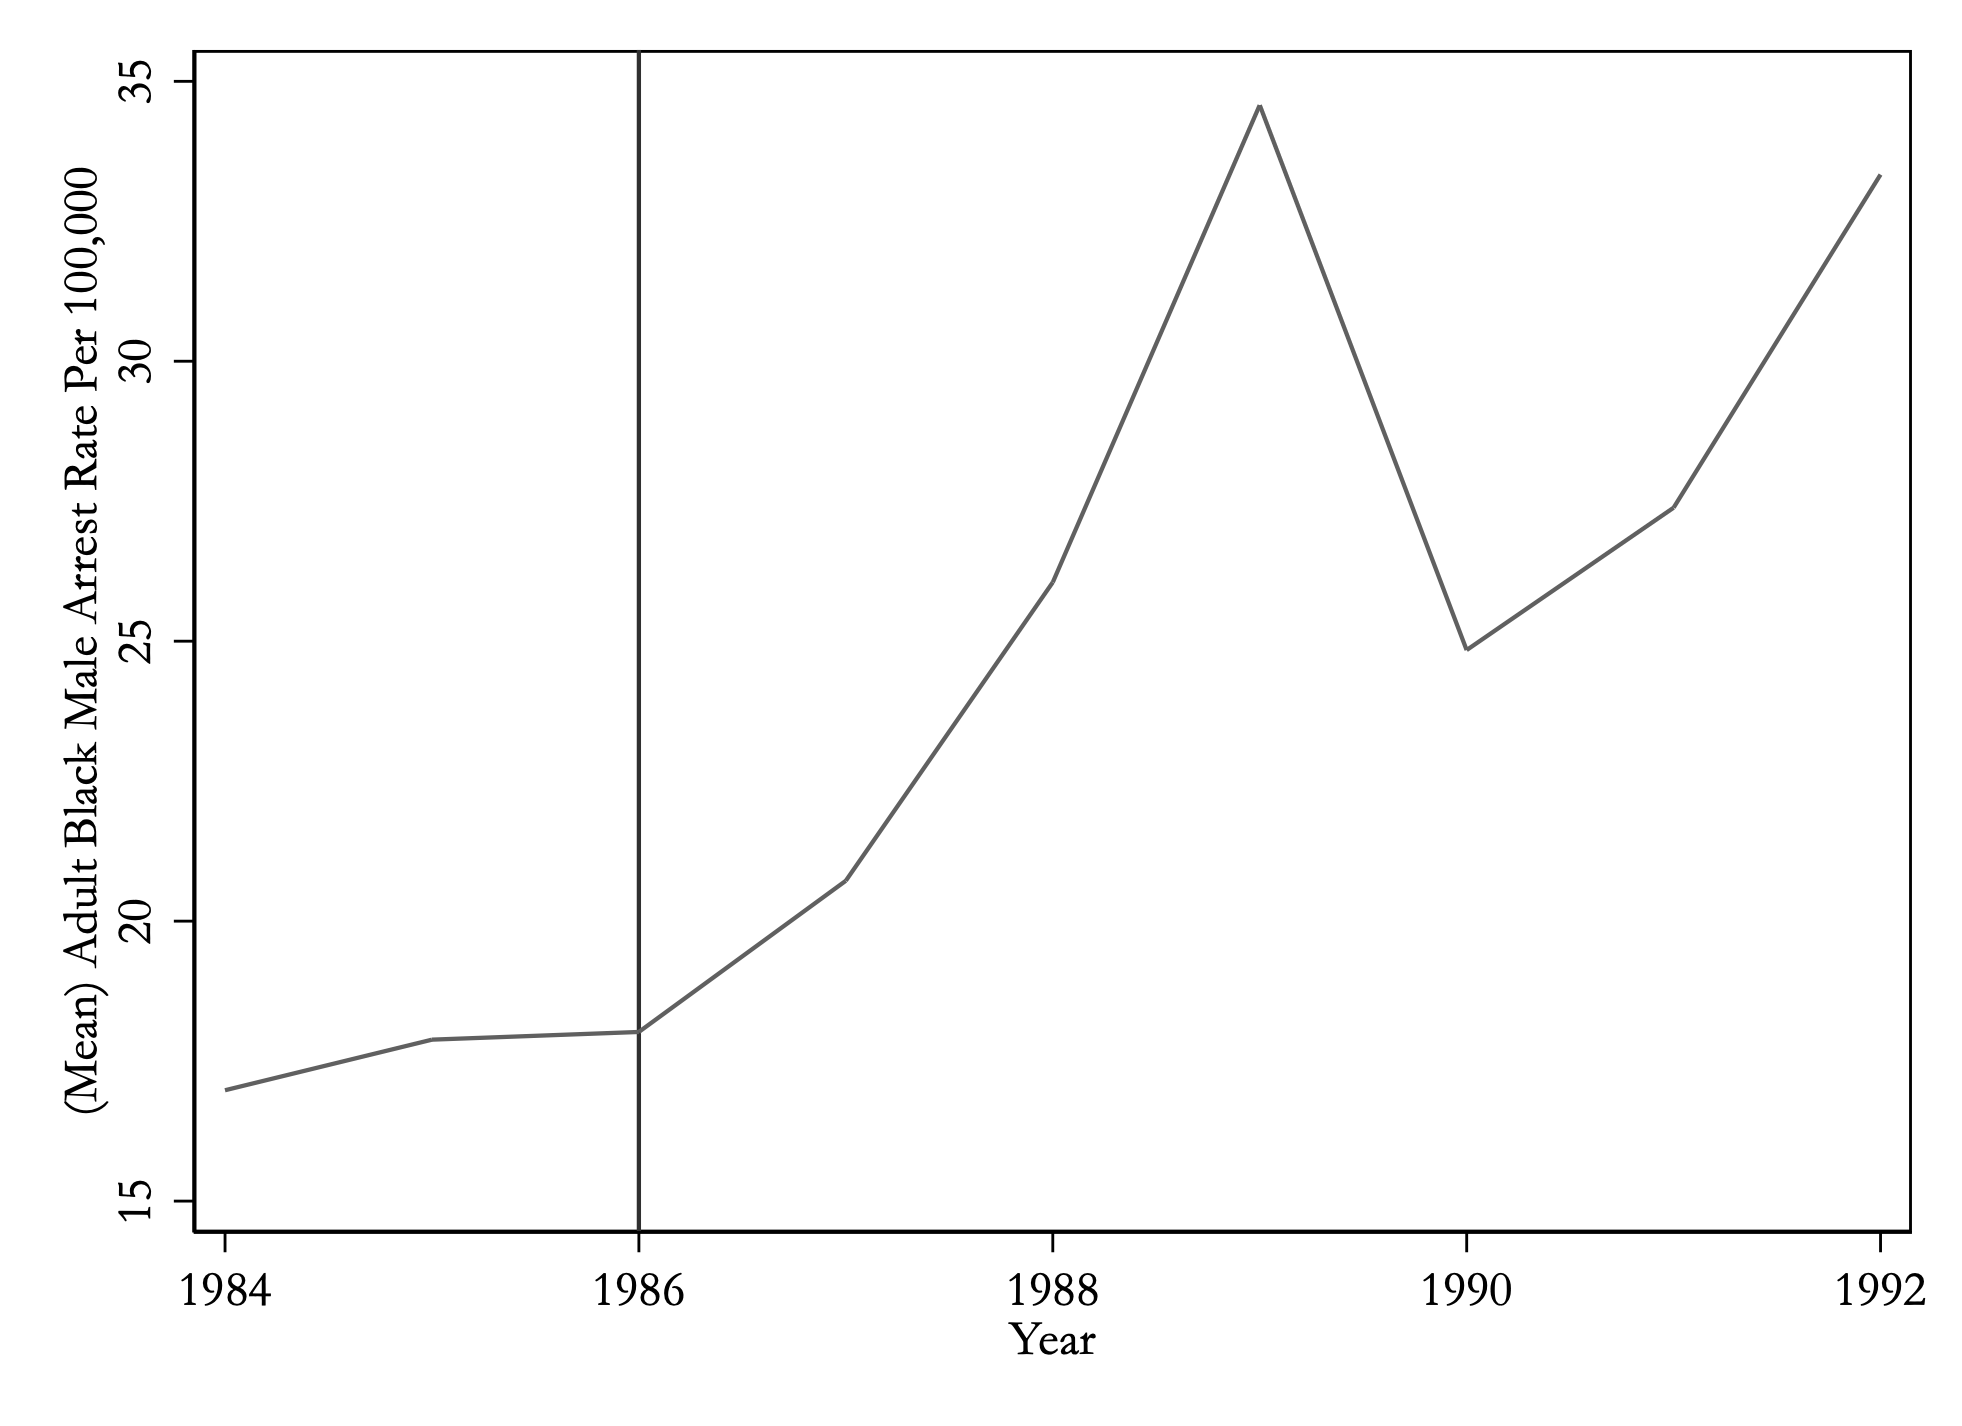
\includegraphics[width=7cm]{pretrends/1986/ab.png} }}%
    \qquad
    \subfloat[\centering 2010]{{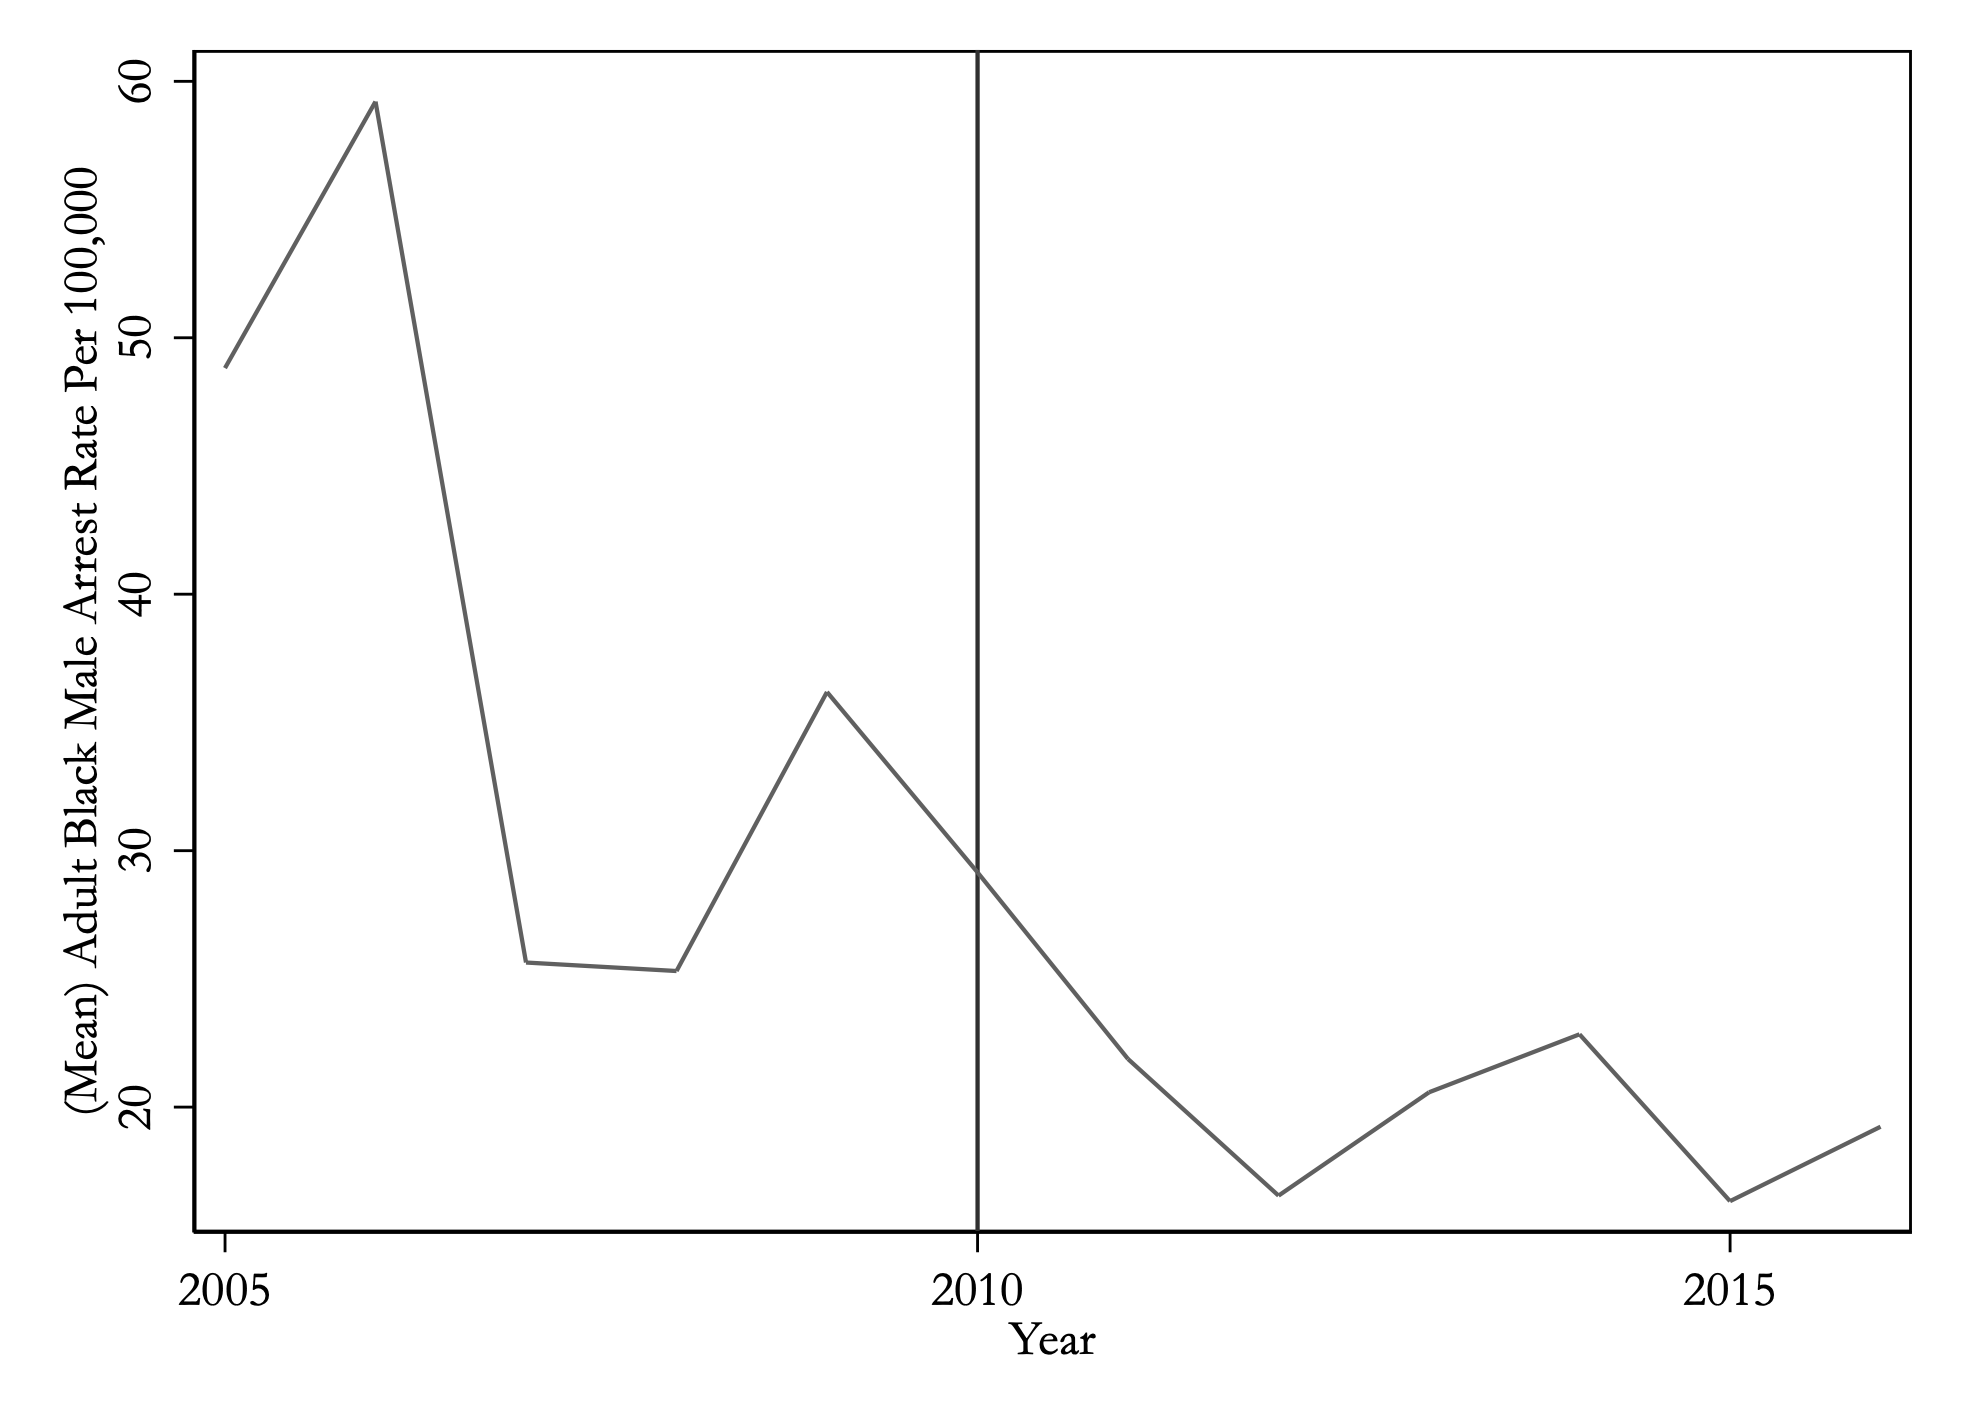
\includegraphics[width=7cm]{pretrends/2010/ab.png} }}%
    \label{fig:raw_ab}%
  \end{figure}
  \begin{figure}[h]
    \centering
    \caption{Juvenile Black Arrest Rate Per 100,000}%
    \subfloat[\centering 1986]{{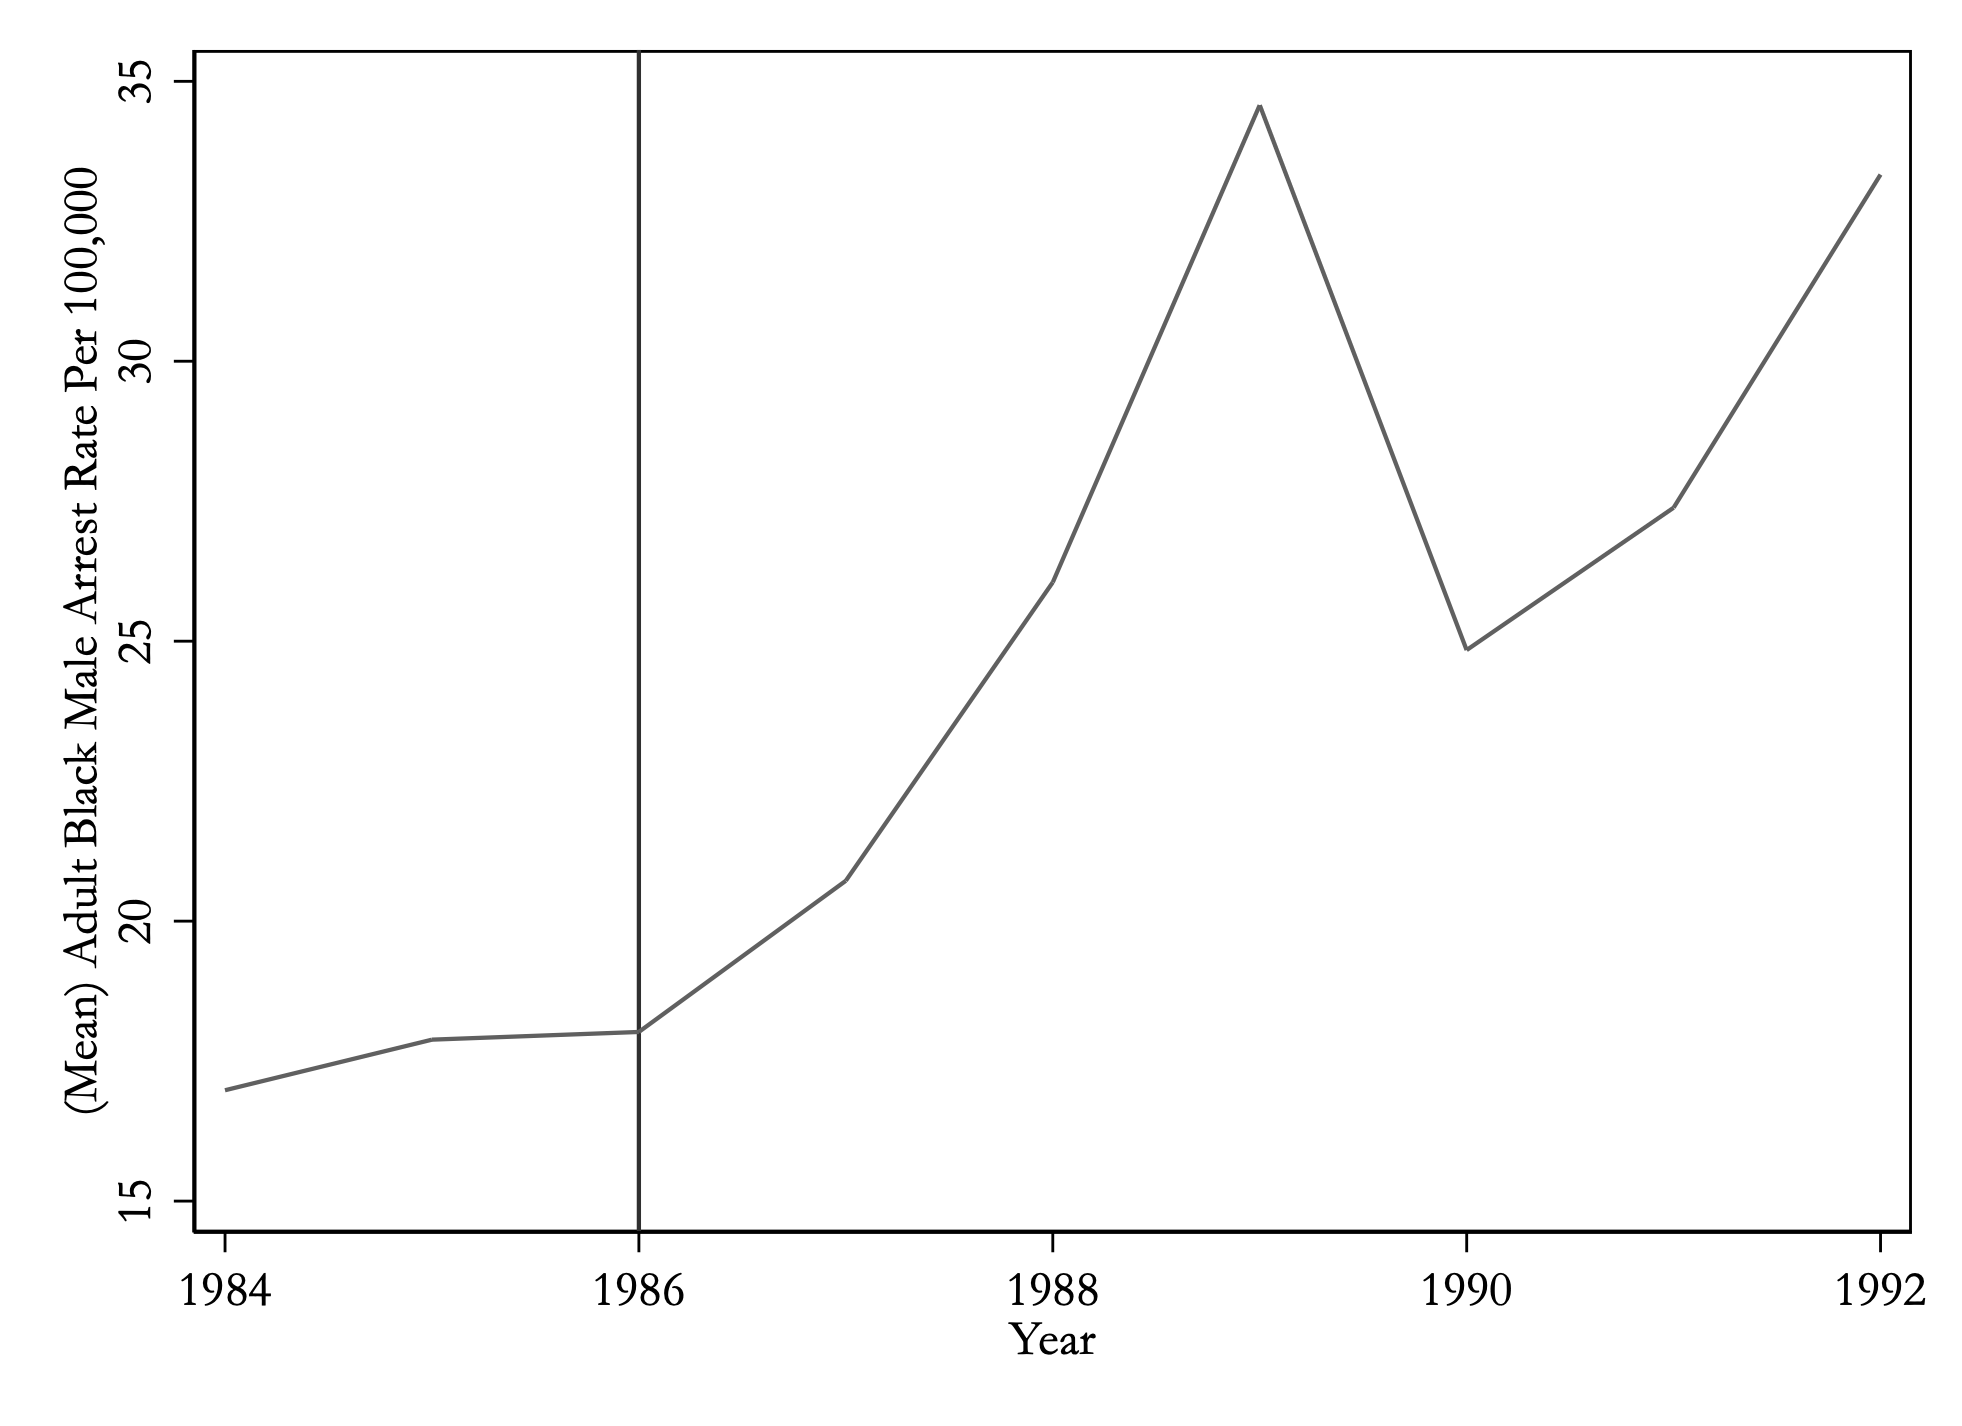
\includegraphics[width=7cm]{pretrends/1986/ab.png} }}%
    \qquad
    \subfloat[\centering 2010]{{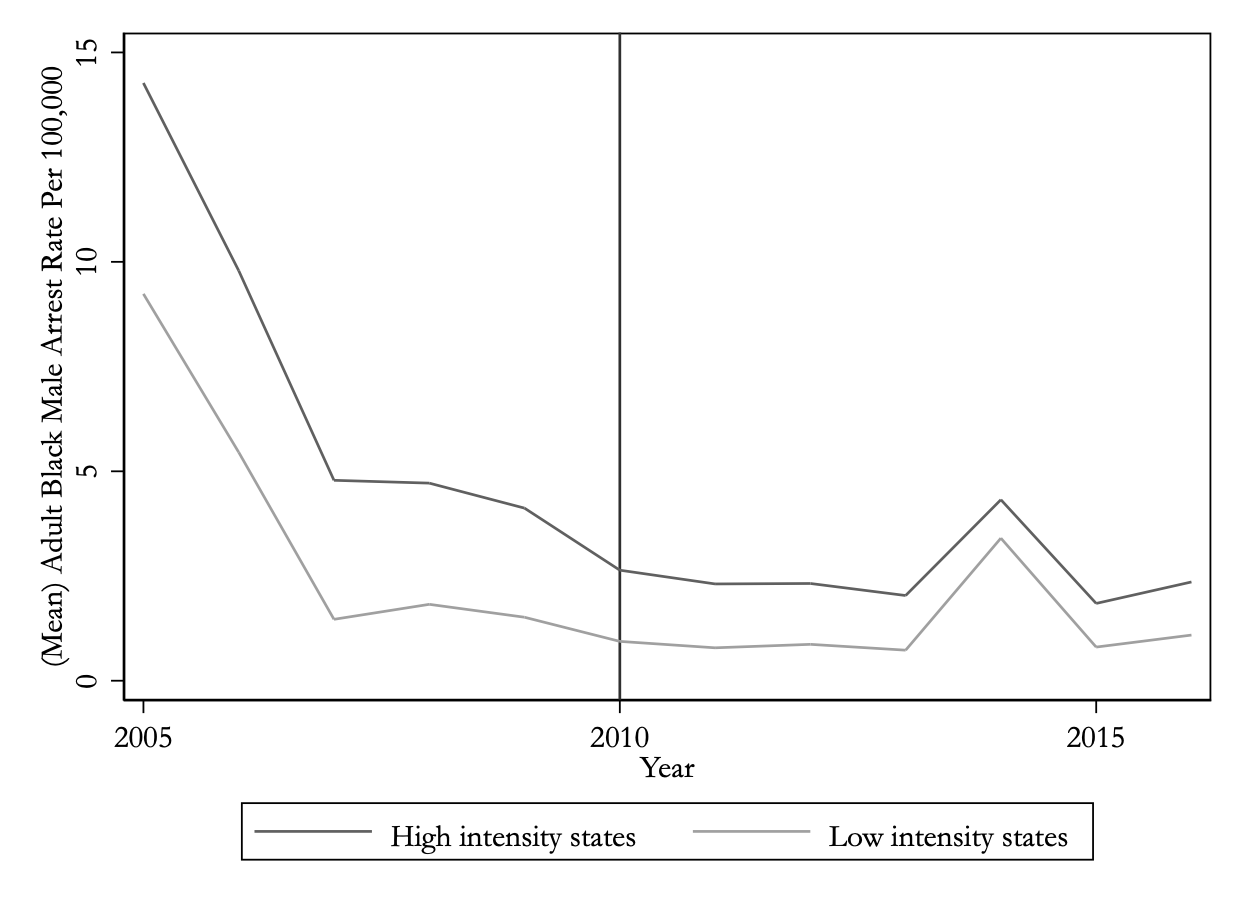
\includegraphics[width=7cm]{pretrends/2010/jb.png} }}%
    \label{fig:raw_jb}%
  \end{figure}

  \begin{footnotesize}
    \noindent Note: These figures report the drug crime arrest rate per 100,000 for black adults and black juveniles separately over time using CPS-UCR merged data from 1984-1992 and 2005-2016. A vertical line is drawn to denote the passage of the Anti-Drug Abuse Act of 1986 and the Fair Sentencing Act of 2010.
  \end{footnotesize}
  
  \clearpage
  
  % High vs low arrest states pre-trends

  \begin{figure}[h]
    \centering
    \caption{College Enrollment By States with High vs Low Black Adult Drug Arrest Rates}%
    \subfloat[\centering 1986]{{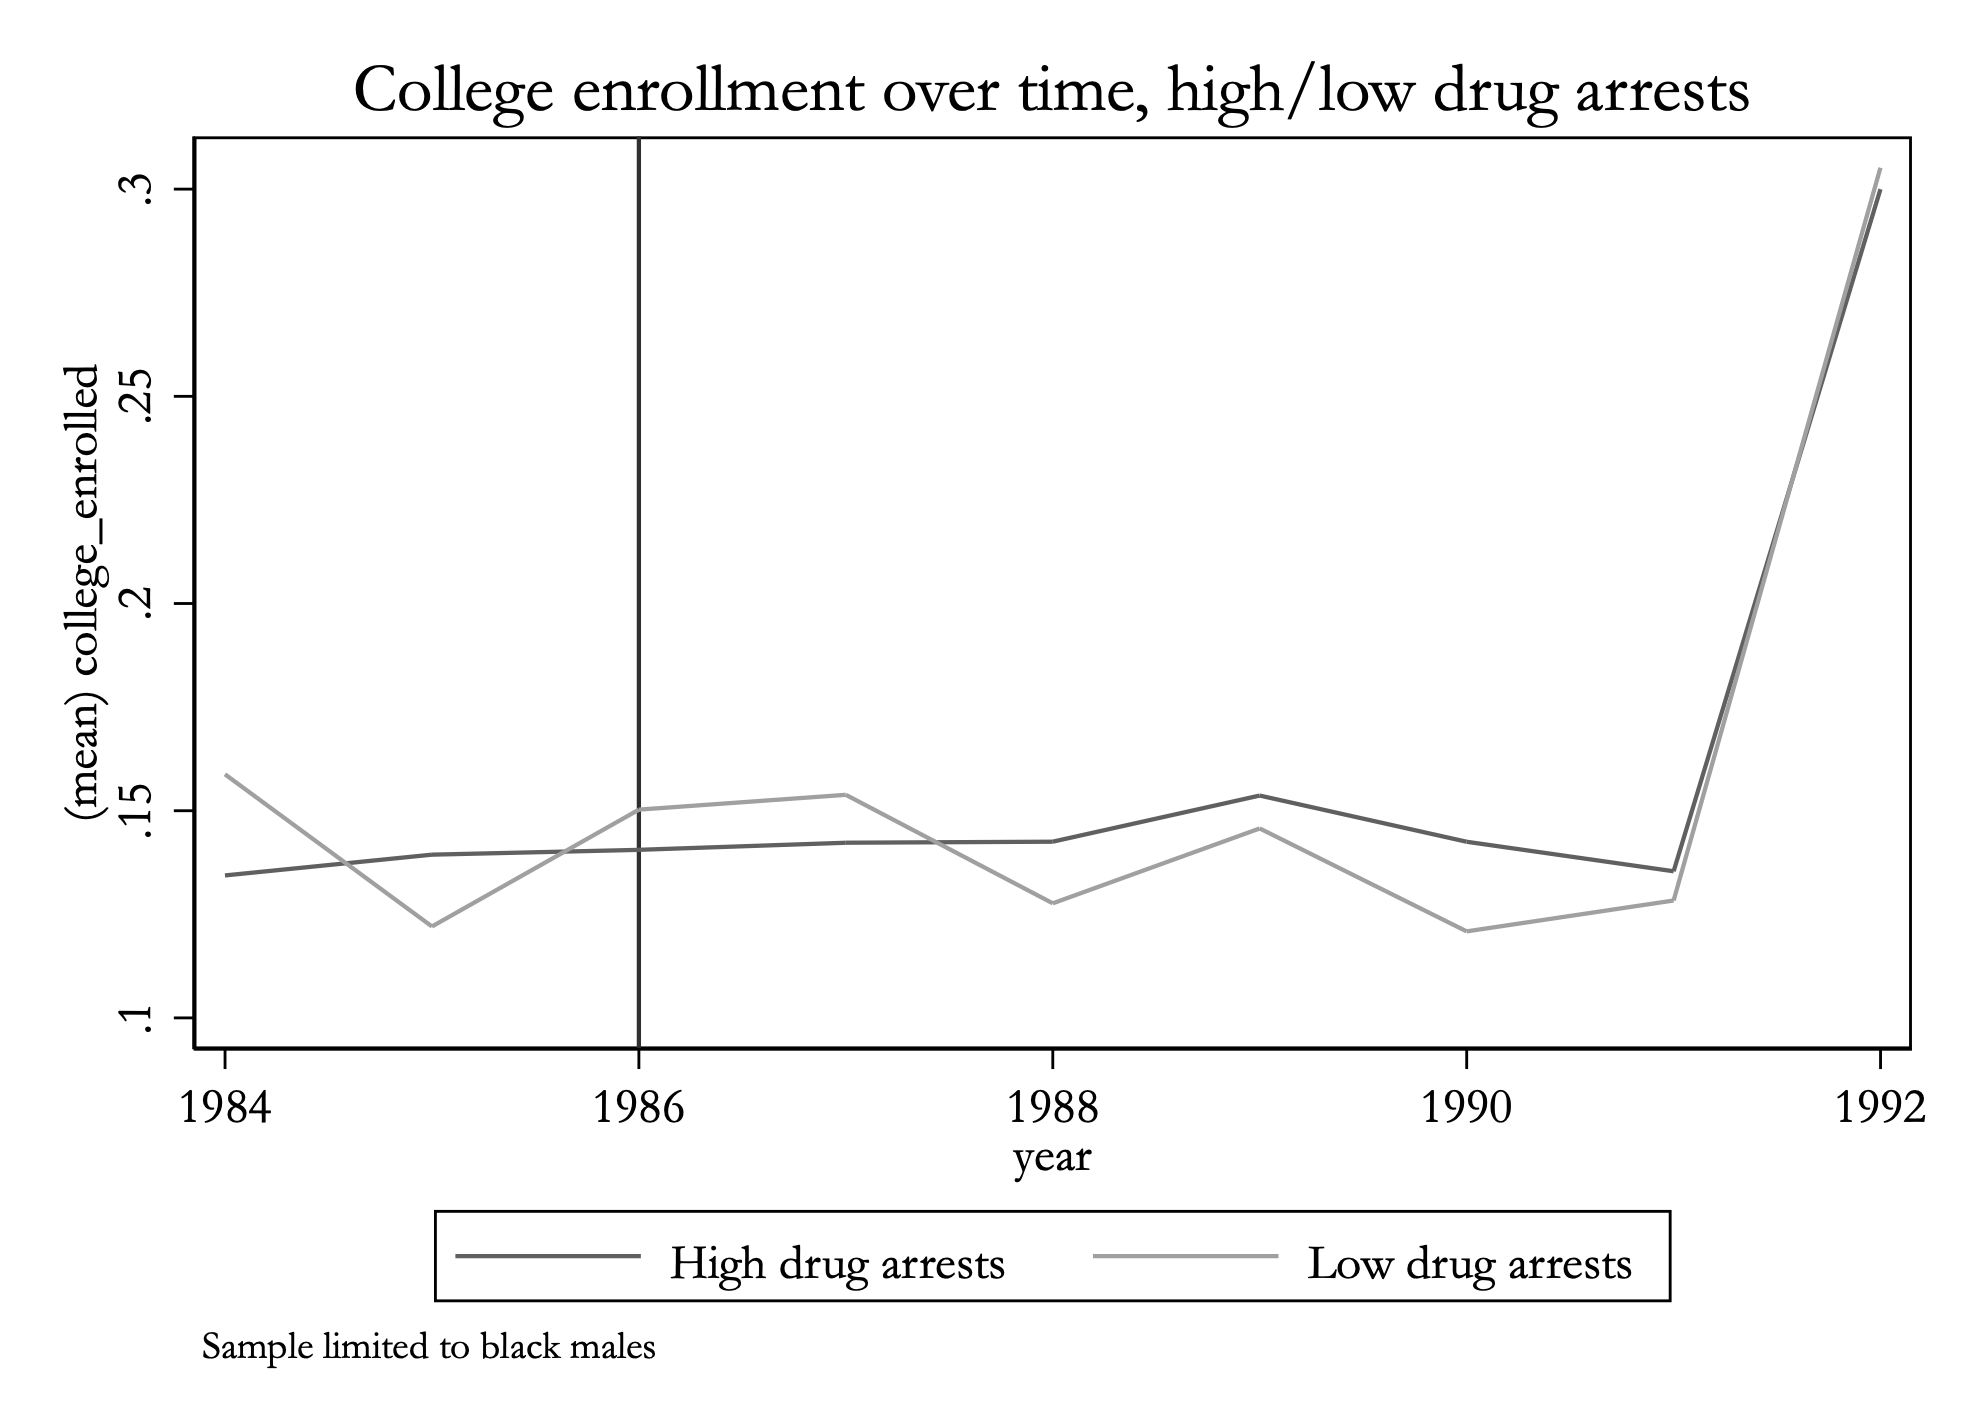
\includegraphics[width=7cm]{pretrends/1986/college_enroll_bydrugarrests_1986.png} }}%
    \qquad
    \subfloat[\centering 2010]{{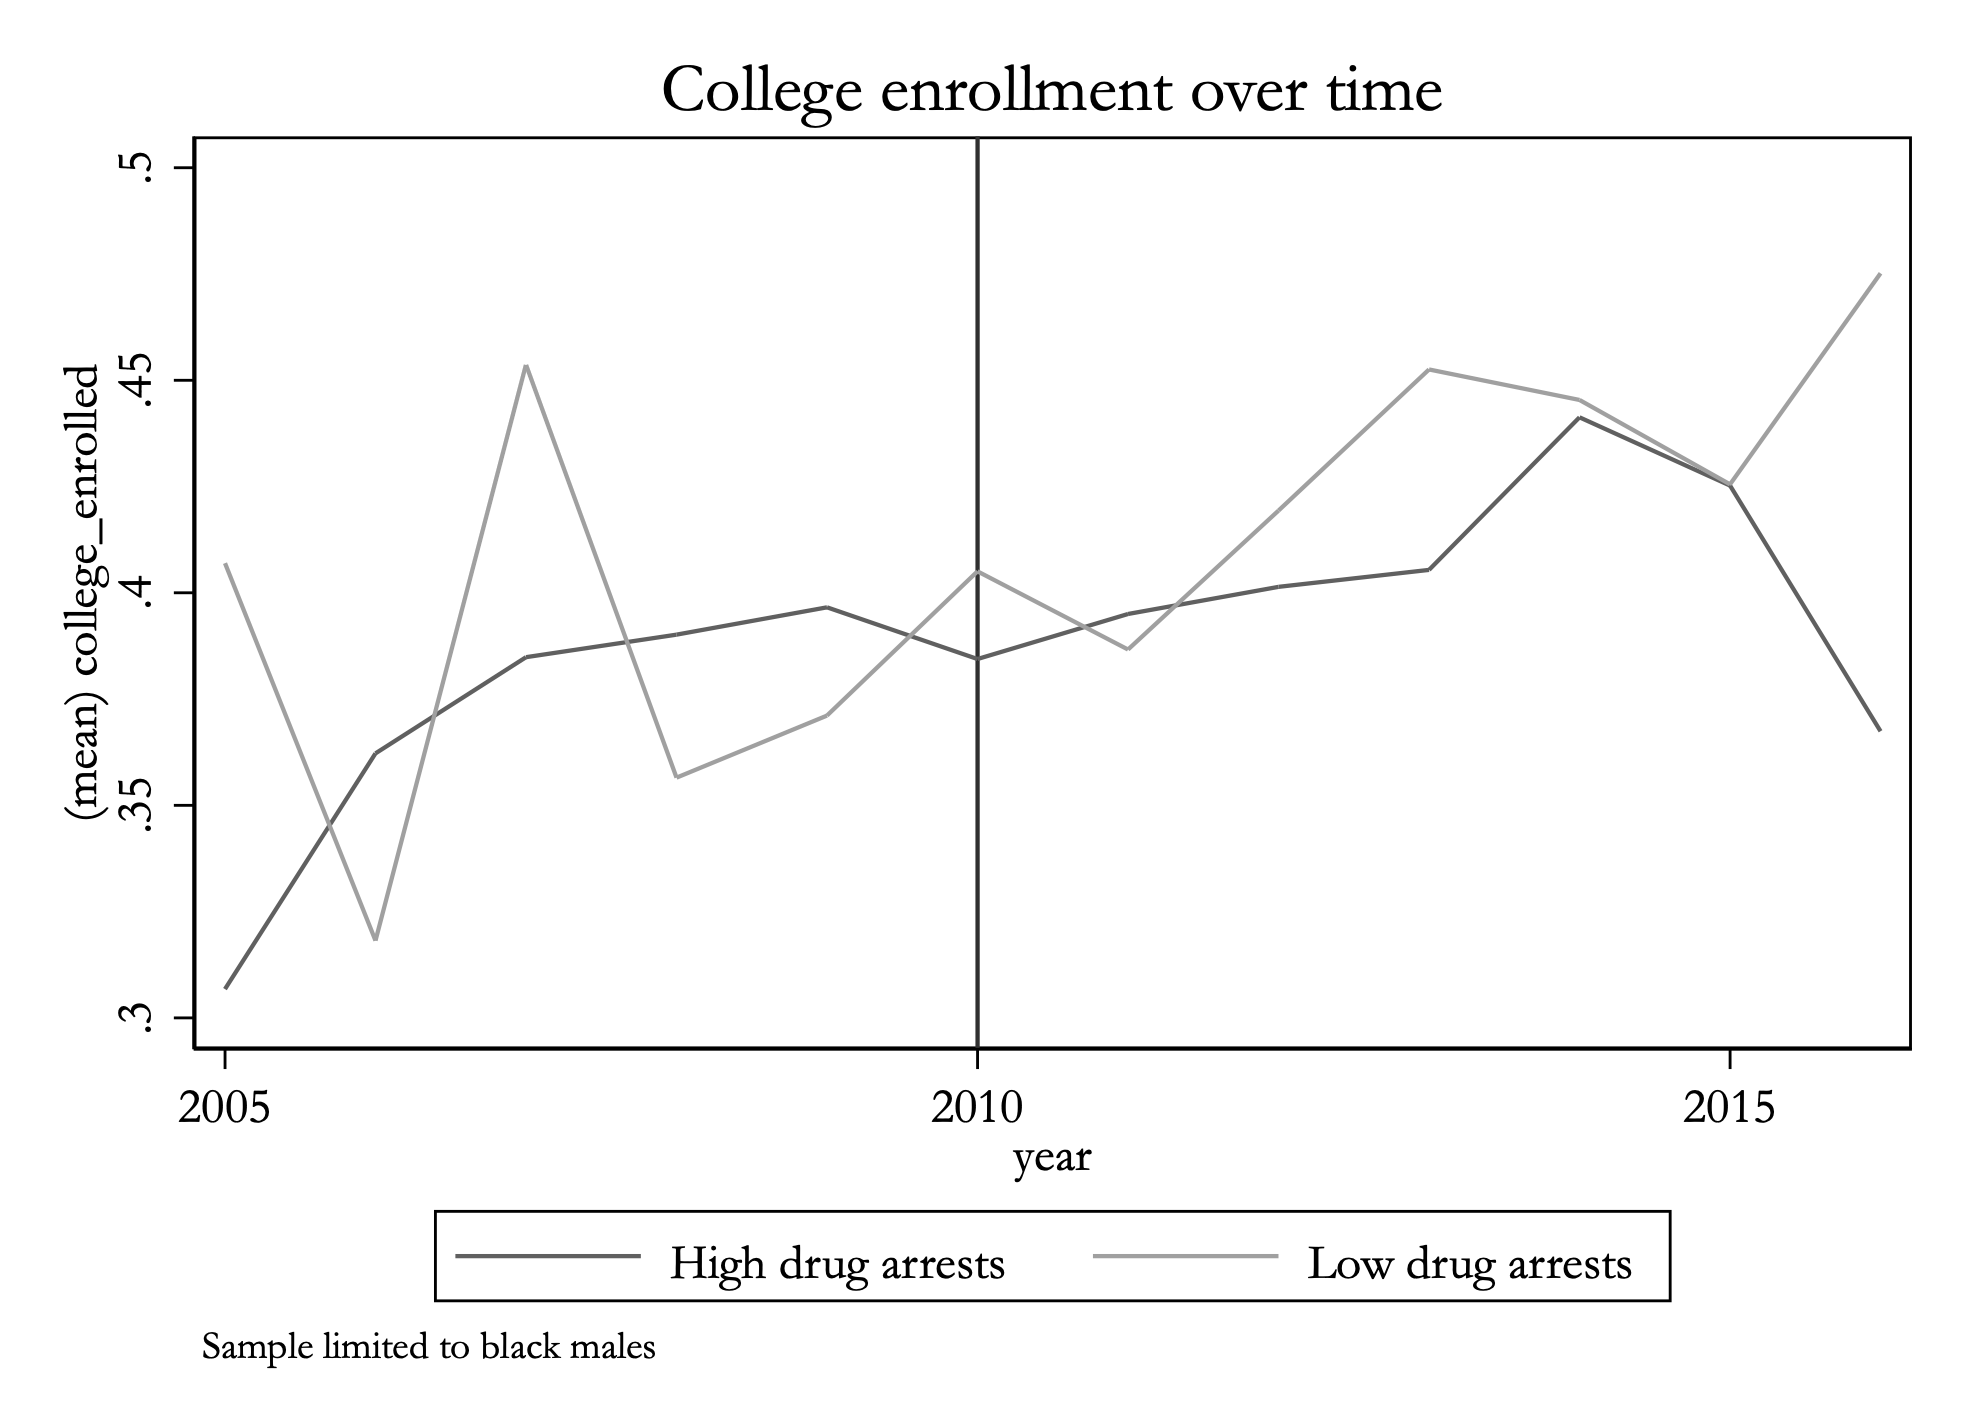
\includegraphics[width=7cm]{pretrends/2010/college_enroll_bydrugarrests_2010.png} }}%
    \label{fig:raw_college_highlowab_1986}%
  \end{figure}
  \begin{figure}[h]
    \centering
    \caption{College Enrollment By States with High vs Low Black Juvenile Drug Arrest Rates}%
    \subfloat[\centering 1986]{{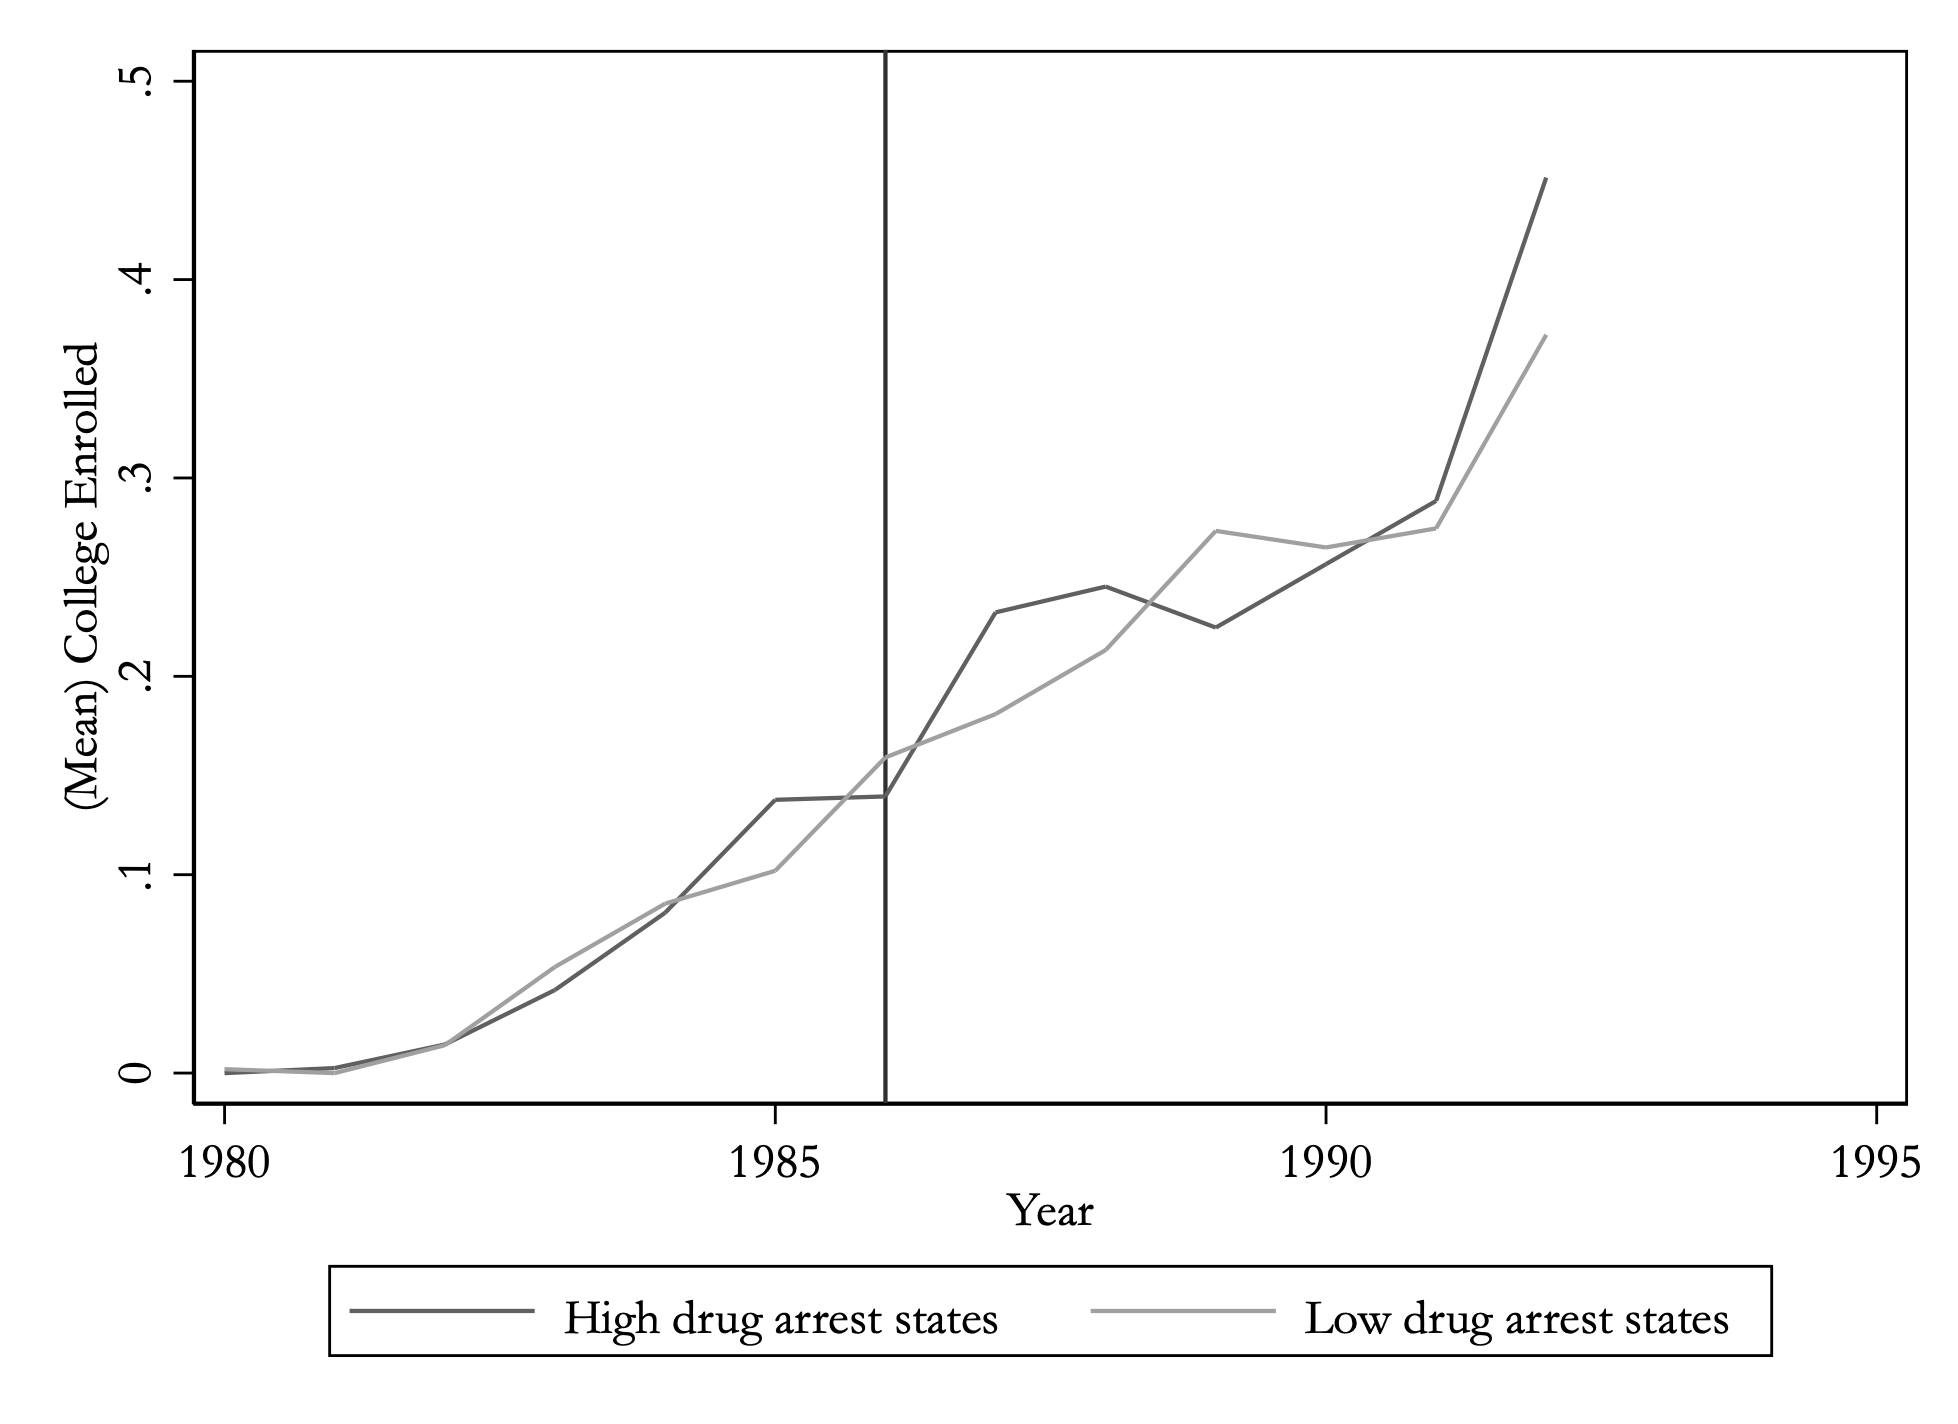
\includegraphics[width=7cm]{pretrends/1986/college_enroll_bydrugarrests_jb_1986.png} }}%
    \qquad
    \subfloat[\centering 2010]{{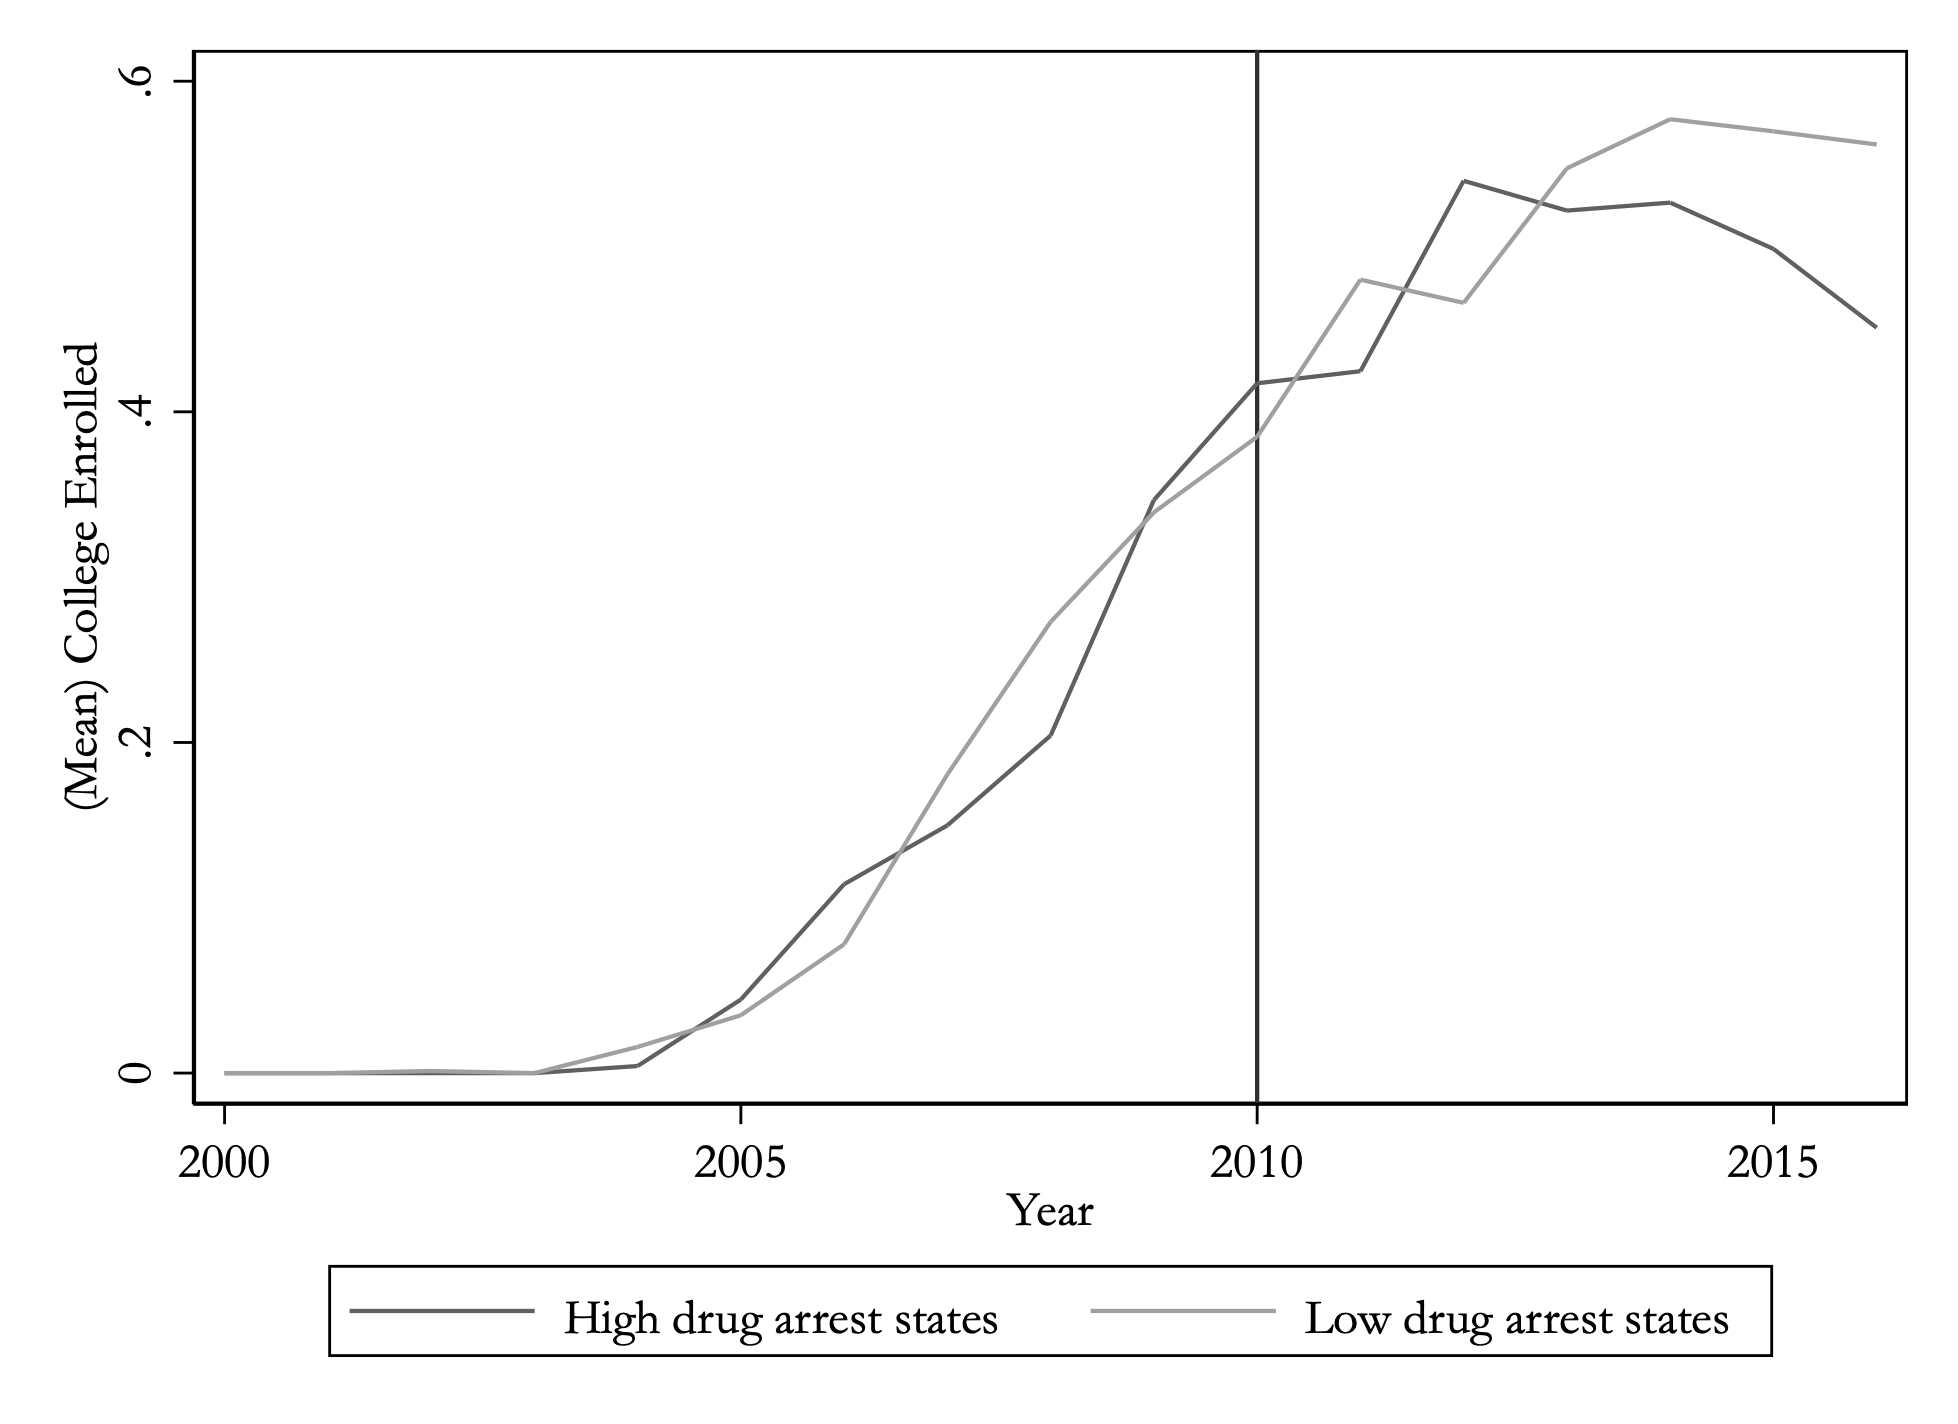
\includegraphics[width=7cm]{pretrends/2010/college_enroll_bydrugarrests_jb_2010.png} }}%
    \label{fig:raw_college_highlowjb_1986}%
  \end{figure}
  
  \begin{footnotesize}
    \noindent Note: These figures report the proportion enrolled in college plotted over time using CPS data from 1984-1992 and 2005-2016 for high black adult/juvenile drug arrest states and low black adult/juvenile drug arrest states, where high black adult/juvenile drug arrest states are defined to be those above the 75th percentile in 1984 and 2008. A vertical line is drawn to denote the passage of the Anti-Drug Abuse Act of 1986 and the Fair Sentencing Act of 2010. The sample is defined as black males aged 18-24 in 1986 and 2010 who were not incarcerated at the time of the survey.
  \end{footnotesize}
  
  \clearpage

  \begin{figure}[h]
    \caption{Black Adult Drug-related Arrest Rate Per 100,000 in 1984} 
    \centering
    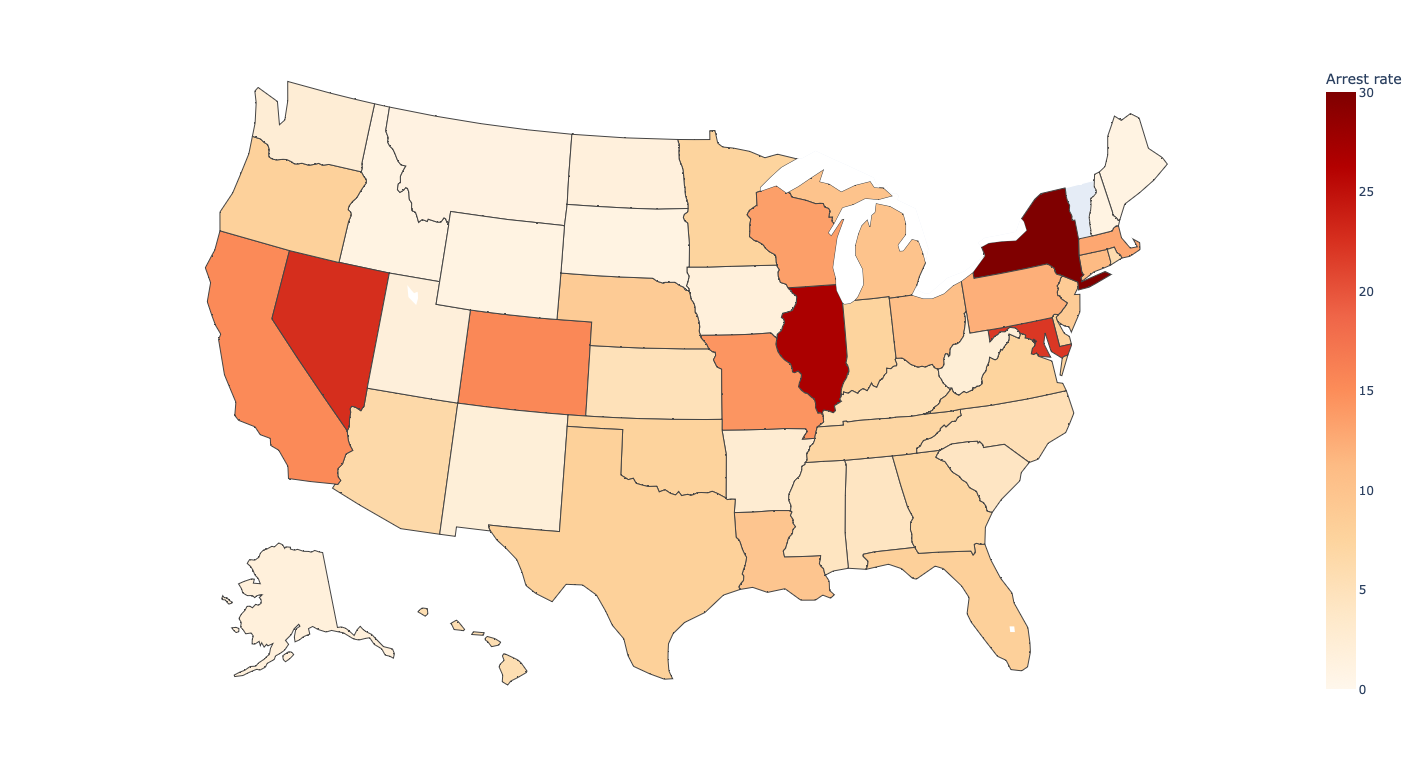
\includegraphics[width=0.8\textwidth]{heatmap/ab1986.png}
    \label{fig:heatmap}
  \end{figure}
  
  \begin{footnotesize}
    \noindent Note: This figure presents a heatmap of the United States at the state level using UCR Program data. The data is from 1984, and I use all drug-related arrests for Black adult men. Although New York's normalized arrest rate is at 48, I capped the maximum at 30 for clarity of states with low normalized drug arrest rates, since the distribution is heavily right-skewed. High drug arrest states are defined as states above the 75th percentile, and the 75th percentile is at 17.4 Black adult arrests per 100,000.
  \end{footnotesize}
  
  \vspace*{8mm}
  
  \begin{figure}[h]
    \centering
    \caption{Distribution of Black Adult Drug-Related Arrest Rates}%
    \subfloat[\centering 1984]{{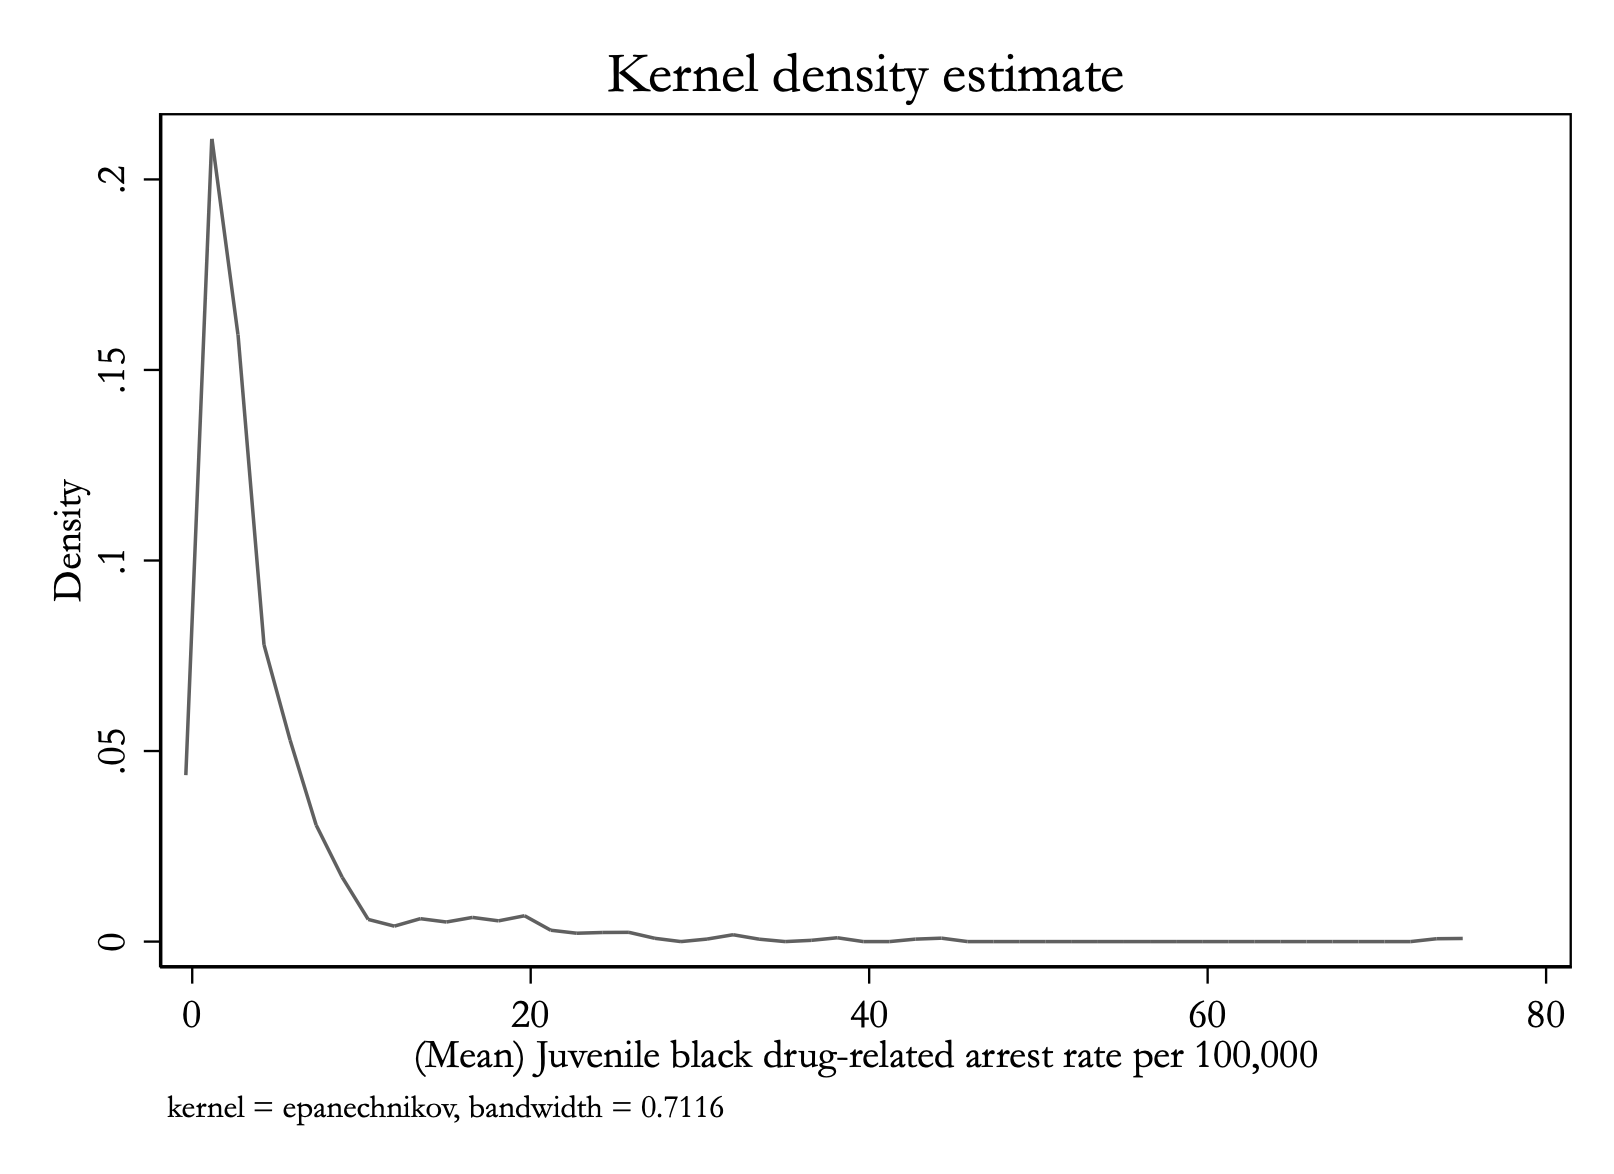
\includegraphics[width=7cm]{descriptive/norm_jb_100000_density_1986} }}%
    \qquad
    \subfloat[\centering 2008]{{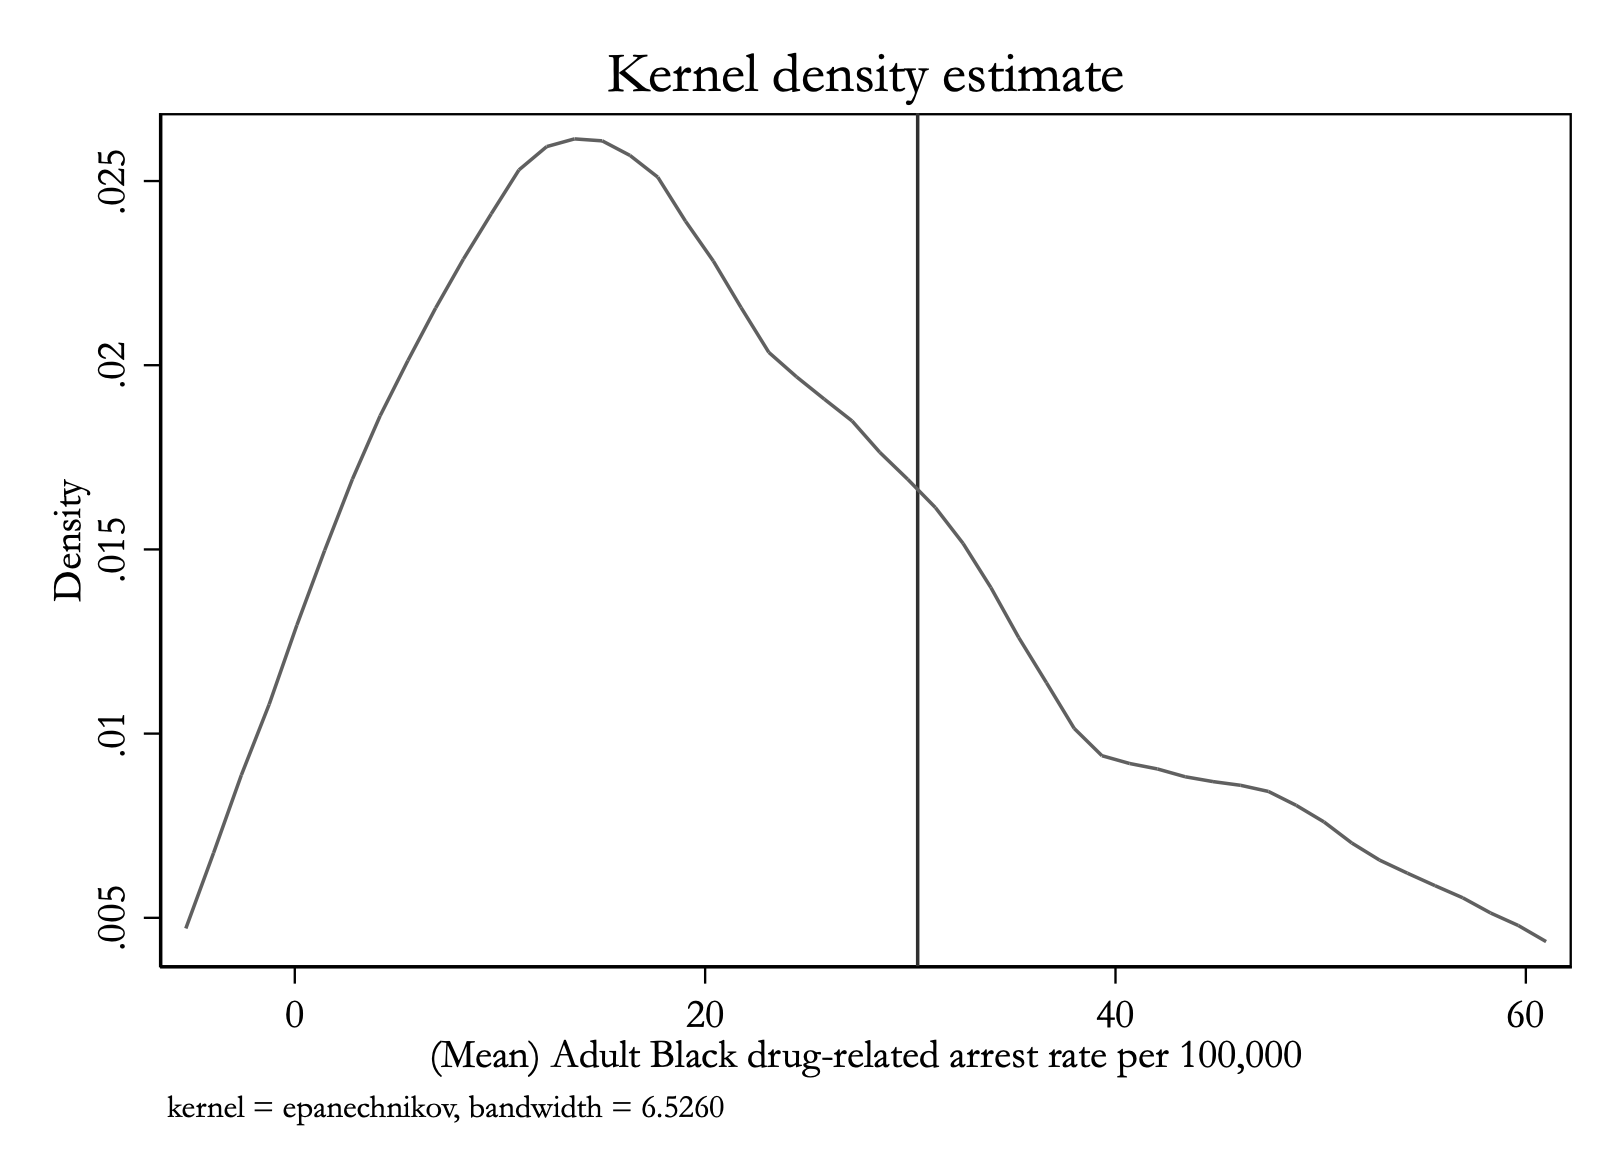
\includegraphics[width=7cm]{descriptive/norm_jb_100000_density_2010.png} }}%
    \label{fig:density_jb}%
  \end{figure}
  \begin{footnotesize}
    \noindent Note: These figures report the kernel density estimates for the normalized drug-related Black adult arrest rate in 1984 and 2008. The vertical line denotes the 75th percentile. Right tail outliers were winsorized at the 95\% level for both figures.
  \end{footnotesize}
  
  \clearpage
     

  % Event study
  \begin{figure}[h]
    \caption{Effect of Anti-Drug Abuse Act on Drug-related Arrest Rate of Adult Black Men, Comparing States with High and Low Black Adult Drug-Related Arrest Rates (with Fixed Effects)}
    \centering
    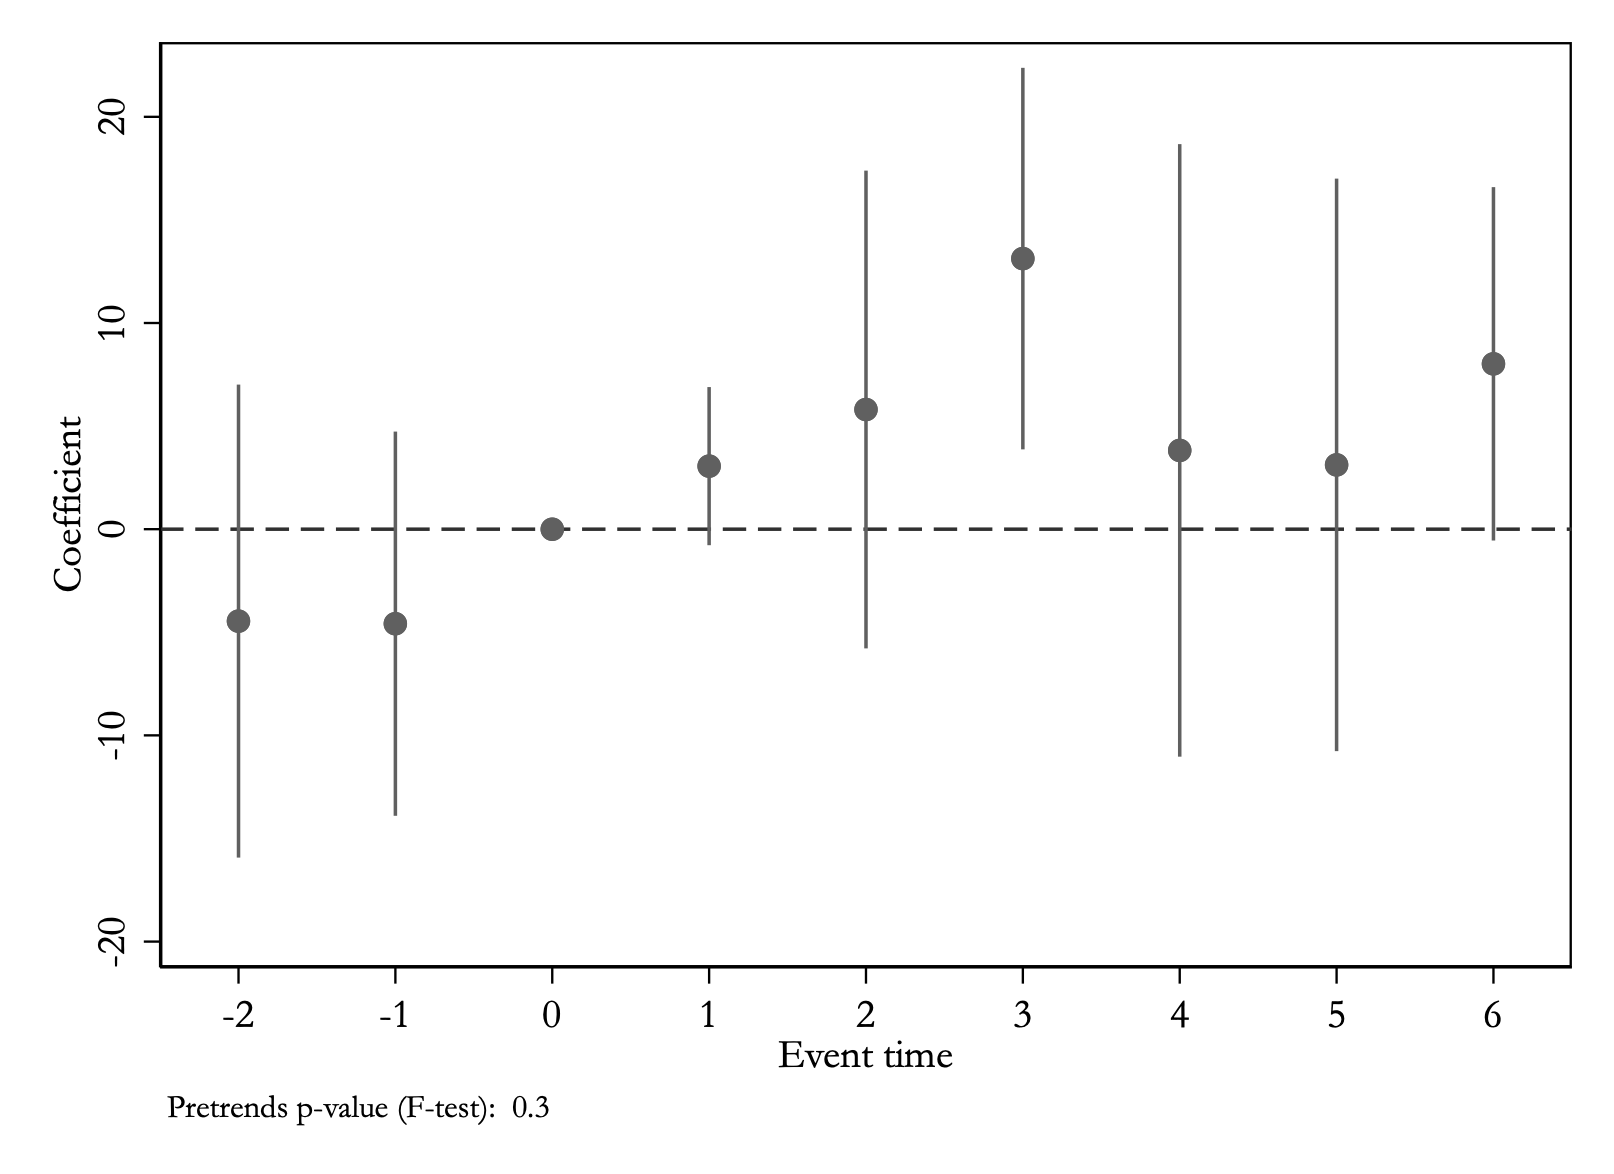
\includegraphics[width=0.7\textwidth]{eventstudy/high_drug_use/high_drug_eventstudy_1986.png}
    \label{fig:ab_es_1986}
  \end{figure}

  \begin{figure}[H]
    \caption{Effect of Anti-Drug Abuse Act on Drug-related Arrest Rate of Adult Black Men, Comparing States with High and Low Black Adult Drug-Related Arrest Rates (without Fixed Effects)}
    \centering
    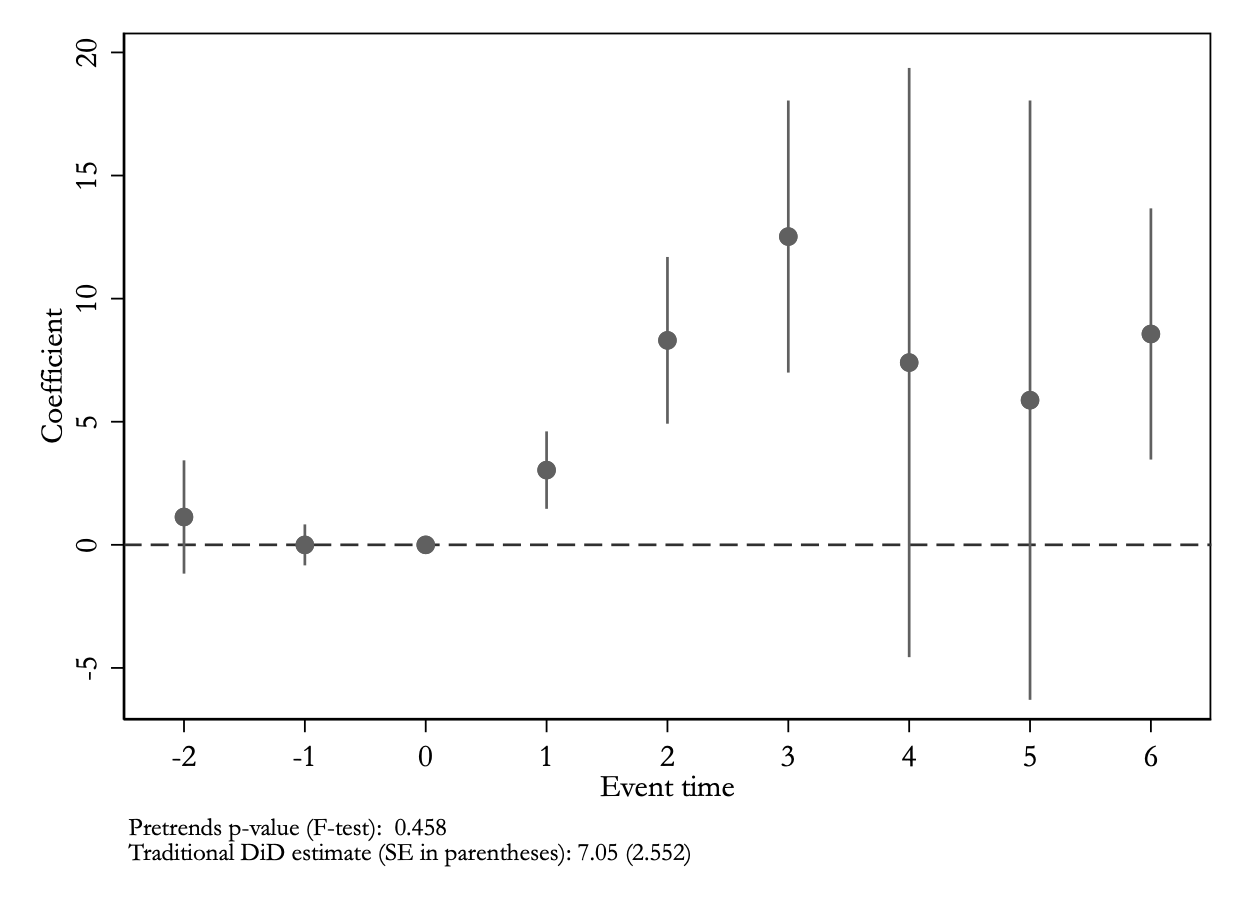
\includegraphics[width=0.7\textwidth]{eventstudy/high_drug_use/high_drug_eventstudy_nofe_1986.png}
    \label{fig:ab_es_1986_nofe}
  \end{figure}
  
  \begin{footnotesize}
    \noindent Note: This figure reports coefficients from the estimation of equation \ref{eq:state_level_es} evaluating the impact of the Anti-Drug Abuse Act of 1986 on arrest rates per 100,000 related to drug violations using CPS and UCR data from 1982-1992. Event time $0 \coloneqq 1986$. The coefficients represent the change in outcomes for high-drug arrest states relative to non-high-drug arrest states, where high black adult drug arrest states are defined to be those above the 75th percentile in 1984. The sample is defined as black males aged 18-24 in 1986 who were not incarcerated at the time of the survey. Control variables include population and unemployment rates at the state-year level. Right tail arrest rate outliers were winsorized at the 95\% level.
  \end{footnotesize}
  
  \clearpage

  \begin{figure}[h]
    \caption{Effect of Anti-Drug Abuse Act on Drug-related Arrest Rate of Black Men, Comparing States with High and Low Black Juvenile Drug-Related Arrest Rate}
    \centering
    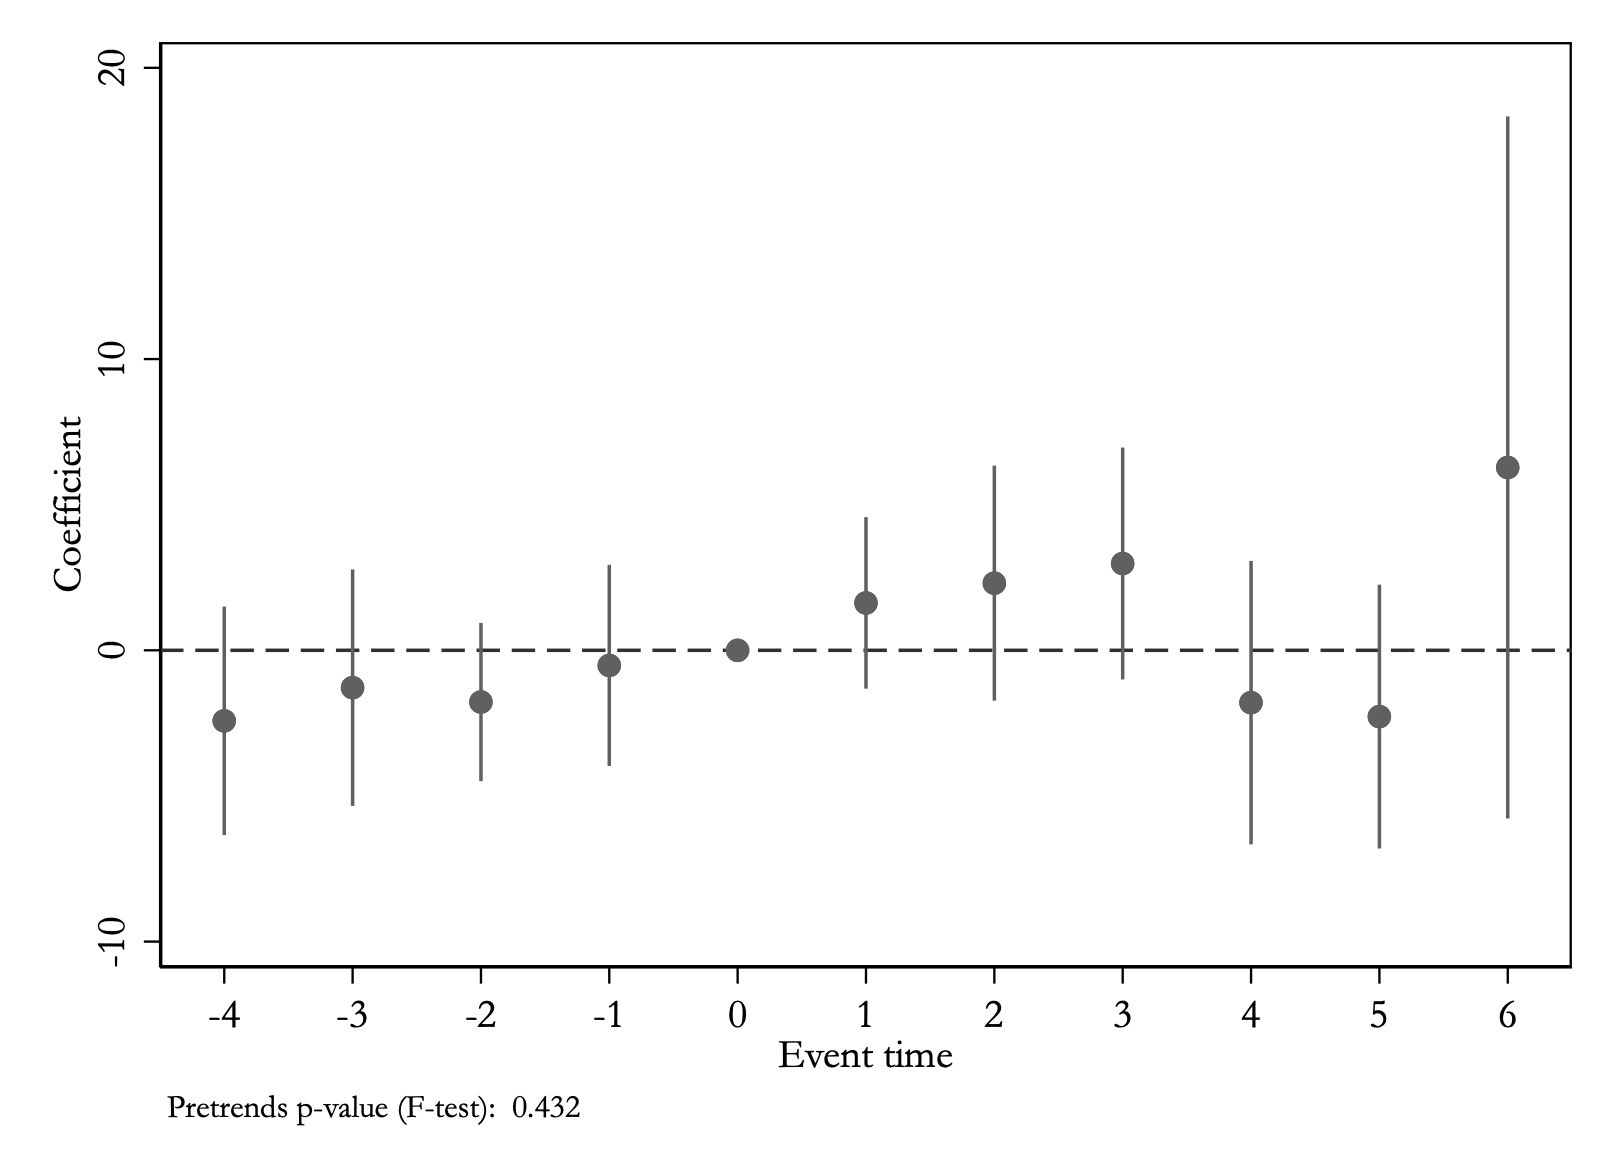
\includegraphics[width=1\textwidth]{eventstudy/high_drug_use/high_drug_eventstudy_1986_jb.png}
    \label{fig:jb_es_1986}
  \end{figure}

  \begin{footnotesize}
    \noindent Note: This figure reports coefficients from the estimation of equation 1 evaluating the impact of the Anti-Drug Abuse Act of 1986 on arrest rates per 100,000 related to drug violations using CPS and UCR data from 1982-1992. Event time $0 \coloneqq 1986$. The coefficients represent the change in outcomes for high black juvenile drug arrest states relative to non-high-drug arrest states, where high-drug arrest states are defined to be those above the 75th percentile in 1984. The sample is defined as black males aged 18-24 in 1986 who were not incarcerated at the time of the survey. Control variables include population and unemployment rates at the state-year level. 
  \end{footnotesize}

  \clearpage

  \begin{figure}[h]
    \centering
    \caption{Additional Pre-trend Testing for Coefficients from Figure 7}%
    \subfloat[\centering Linear pre-trend]{{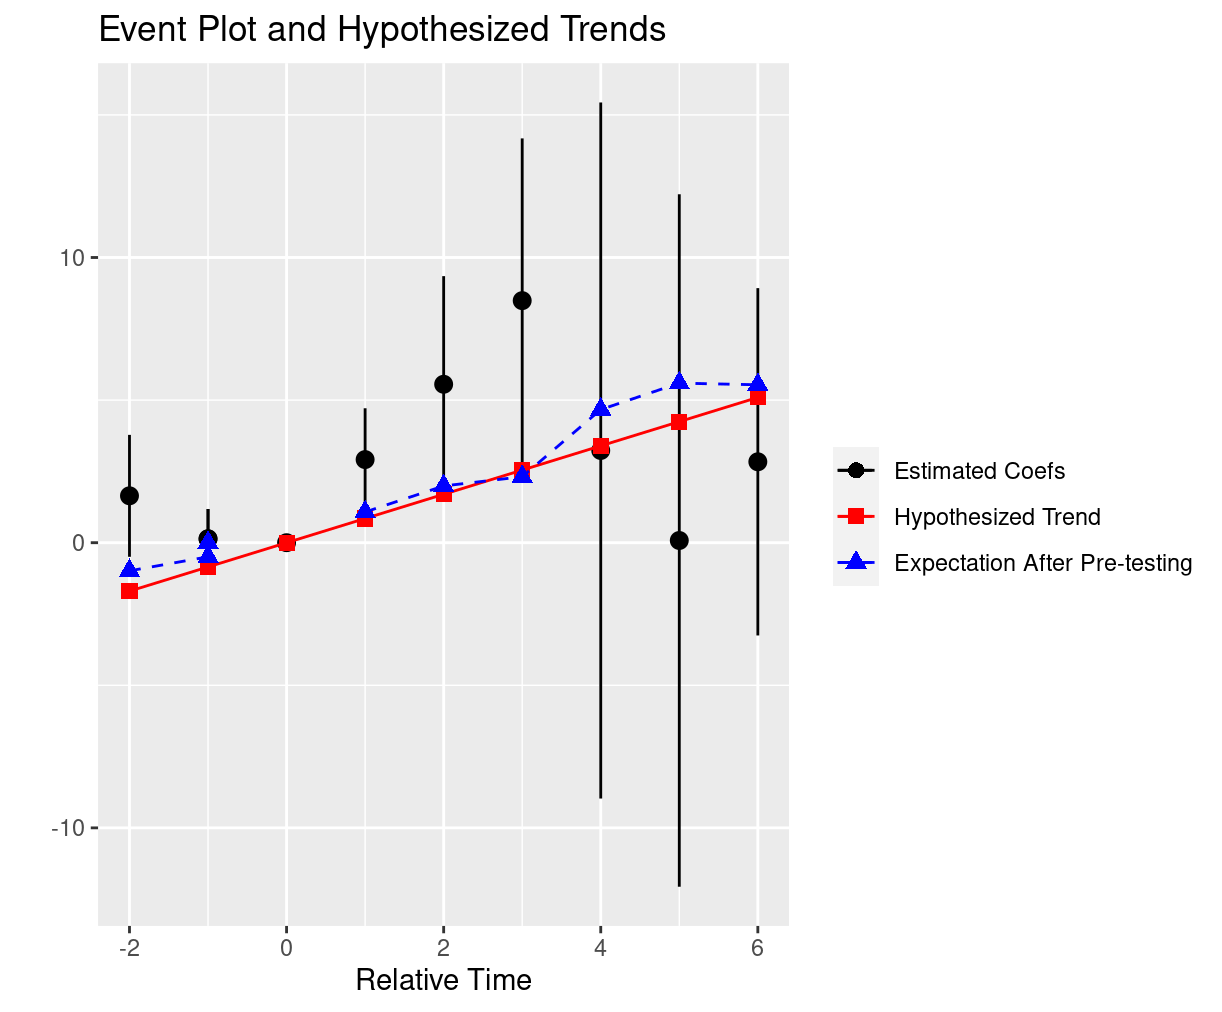
\includegraphics[width=7cm]{pretrends/power/firststage_linear_ab1986.png} }}%
    \qquad
    \subfloat[\centering Quadratic pre-trend]{{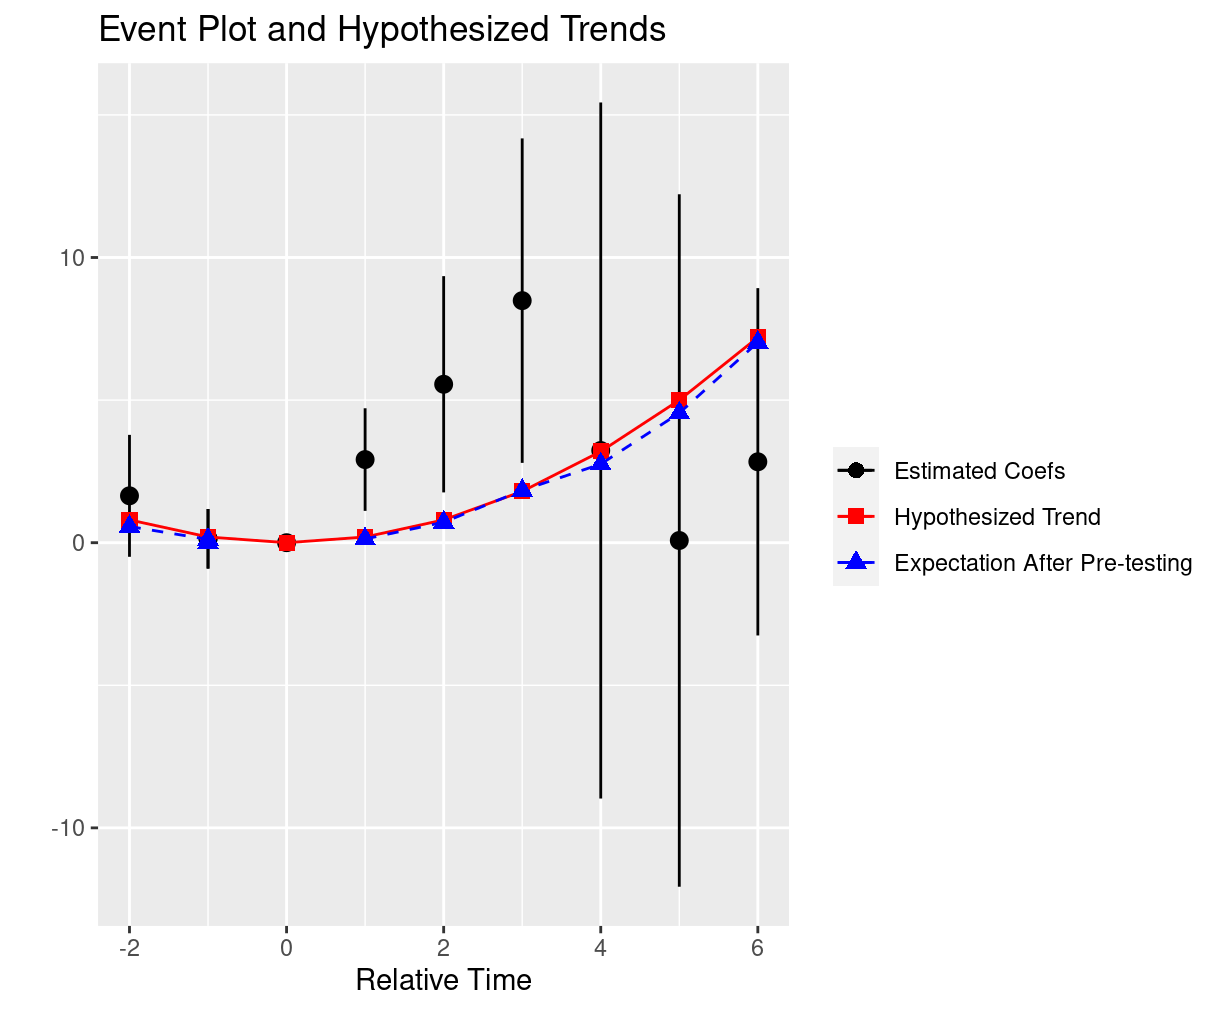
\includegraphics[width=7cm]{pretrends/power/firststage_quad_ab1986.png} }}%
    \label{fig:pre-trends_roth}%
  \end{figure}

  \begin{footnotesize}
    \noindent Note: These two figures were constructed using an R package written by Roth (2022). The figures and pre-trend statistics were calculated using the estimated coefficients from Figure 7 and their corresponding covariance matrixes. The slope in Figure A was constructed such that the power would be about 0.5, while the quadratic trend in Figure B was chosen visually. The blue expectation after pretesting coefficients represents the expected value of the coefficients conditional on passing the pre-test under the hypothesized trend.

    Figure A statistics: 1) power = 0.499, 2) Bayes Factor = 0.549, 3) likelihood ratio = 0.033.

    Figure B statistics: 1) power = 0.155, 2) Bayes Factor = 0.928, 3) likelihood ratio = 2.323.
  \end{footnotesize}

  \clearpage
  
  \begin{figure}[h]
    \centering
    \caption{Effect of Fair Sentencing Act on Drug-related Arrest Rate of Adult Black Men, Comparing High and Low-Intensity States}%
    \subfloat[\centering Using adults arrests]{{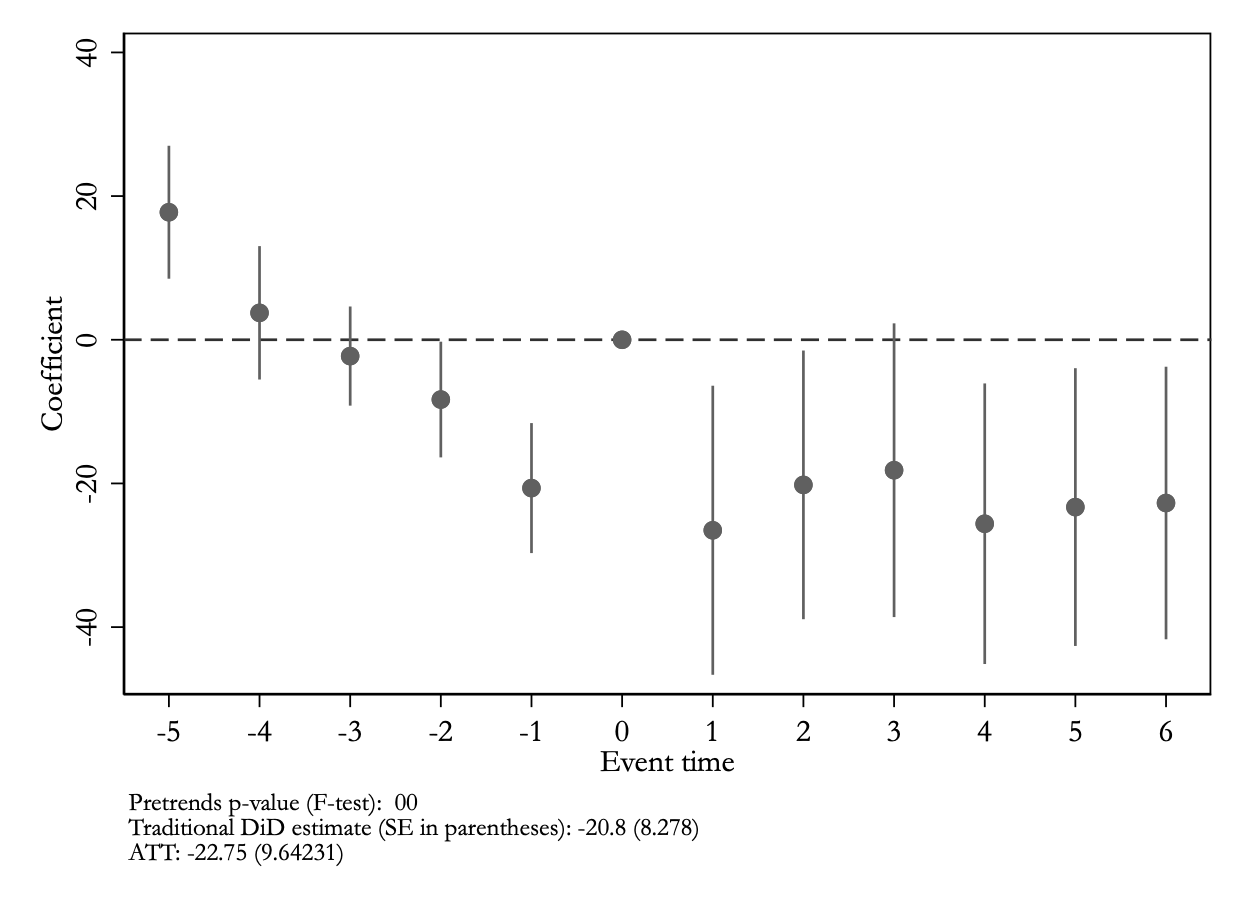
\includegraphics[width=7cm]{eventstudy/high_drug_use/high_drug_eventstudy_2010_ab.png} }}%
    \qquad
    \subfloat[\centering Using juvenile arrests]{{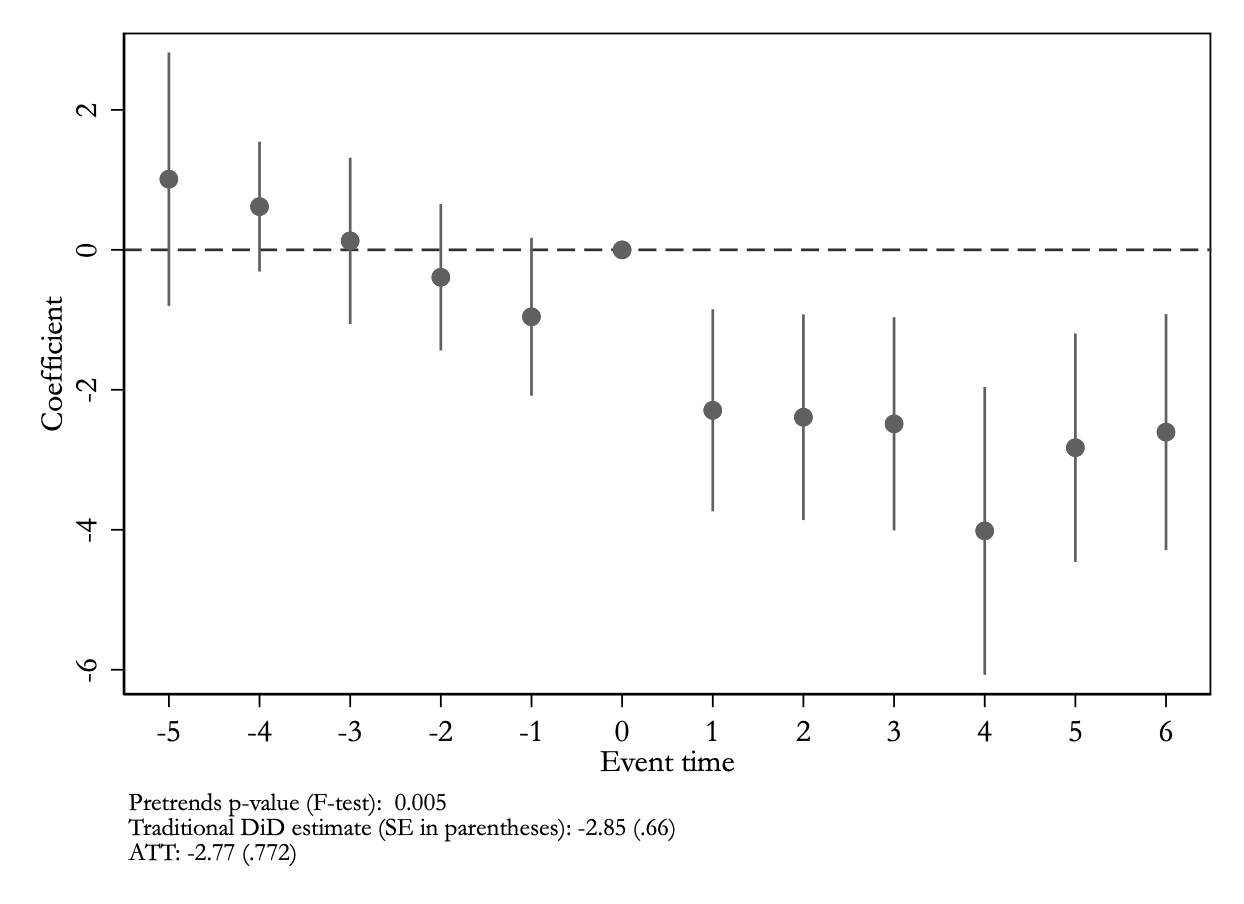
\includegraphics[width=7cm]{eventstudy/high_drug_use/high_drug_eventstudy_2010_jb.png} }}%
    \label{fig:fs_es_2010}%
  \end{figure}


  \begin{footnotesize}
    \noindent Note: These figures report coefficients from the estimation of equation 1 evaluating the impact of the Fair Sentencing Act of 2010 on arrest rates per 100,000 related to drug violations using CPS-UCR merged data from 2005-2015. Figure A defines high-intensity states using Black adult arrests, while Figure B defines high-intensity states using Black juvenile arrests. Event time $0 \coloneqq 2010$. The coefficients represent the change in outcomes for high black adult drug arrest states relative to non-high-drug arrest states, where high-drug arrest states are defined to be those above the 75th percentile in 2008. The sample is defined as black males aged 18-24 in 2010 who were not incarcerated at the time of the survey. Control variables include population and unemployment rates at the state-year level. 
  \end{footnotesize}

\clearpage 

\begin{figure}[h]
  \centering
  \caption{Effect of Anti-Drug Abuse Act on the College Enrollment Rate of Adult Black Men, Comparing High and Low-Intensity States}%
  \subfloat[\centering Using adults arrests]{{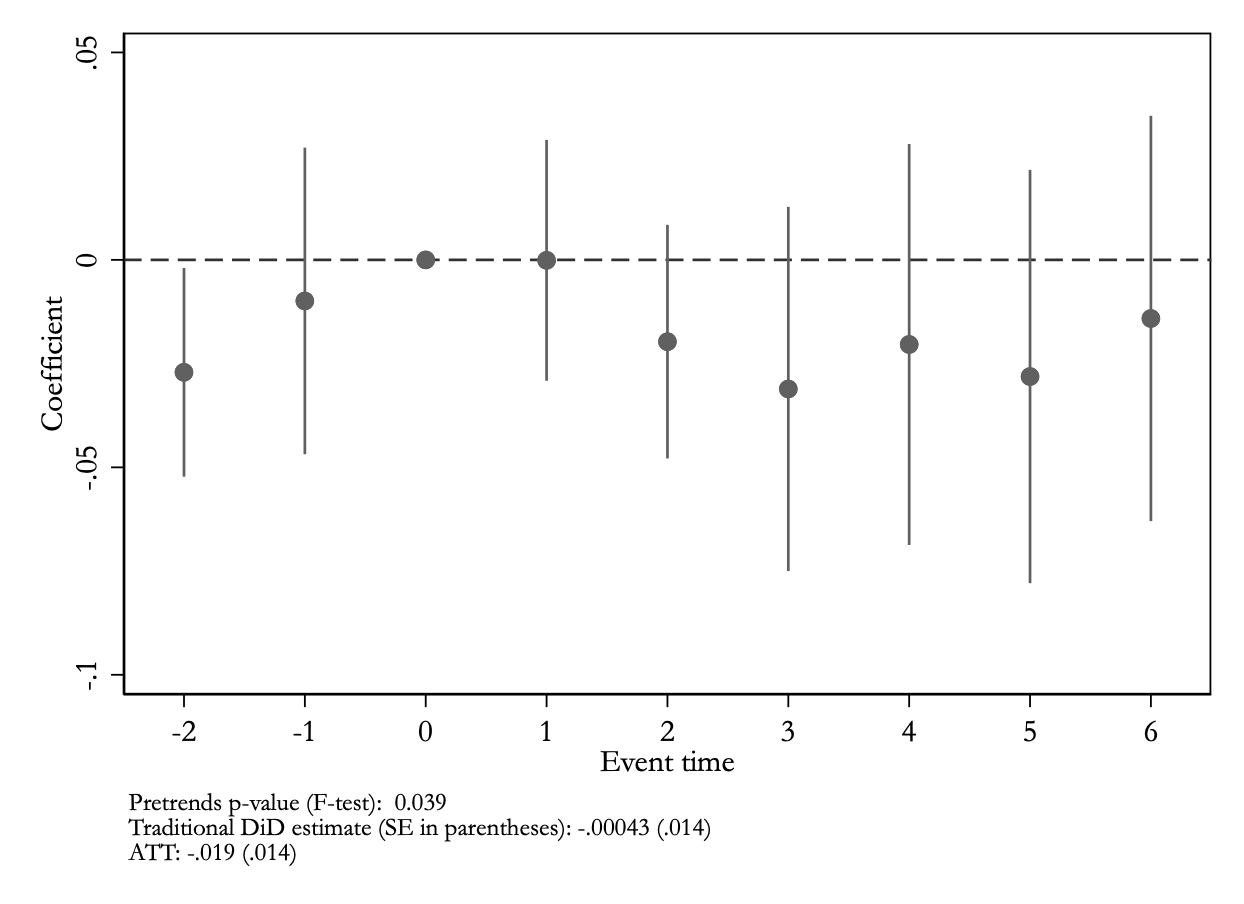
\includegraphics[width=7cm]{eventstudy/high_drug_use/reducedform_ab1986.png} }}%
  \qquad
  \subfloat[\centering Using juvenile arrests]{{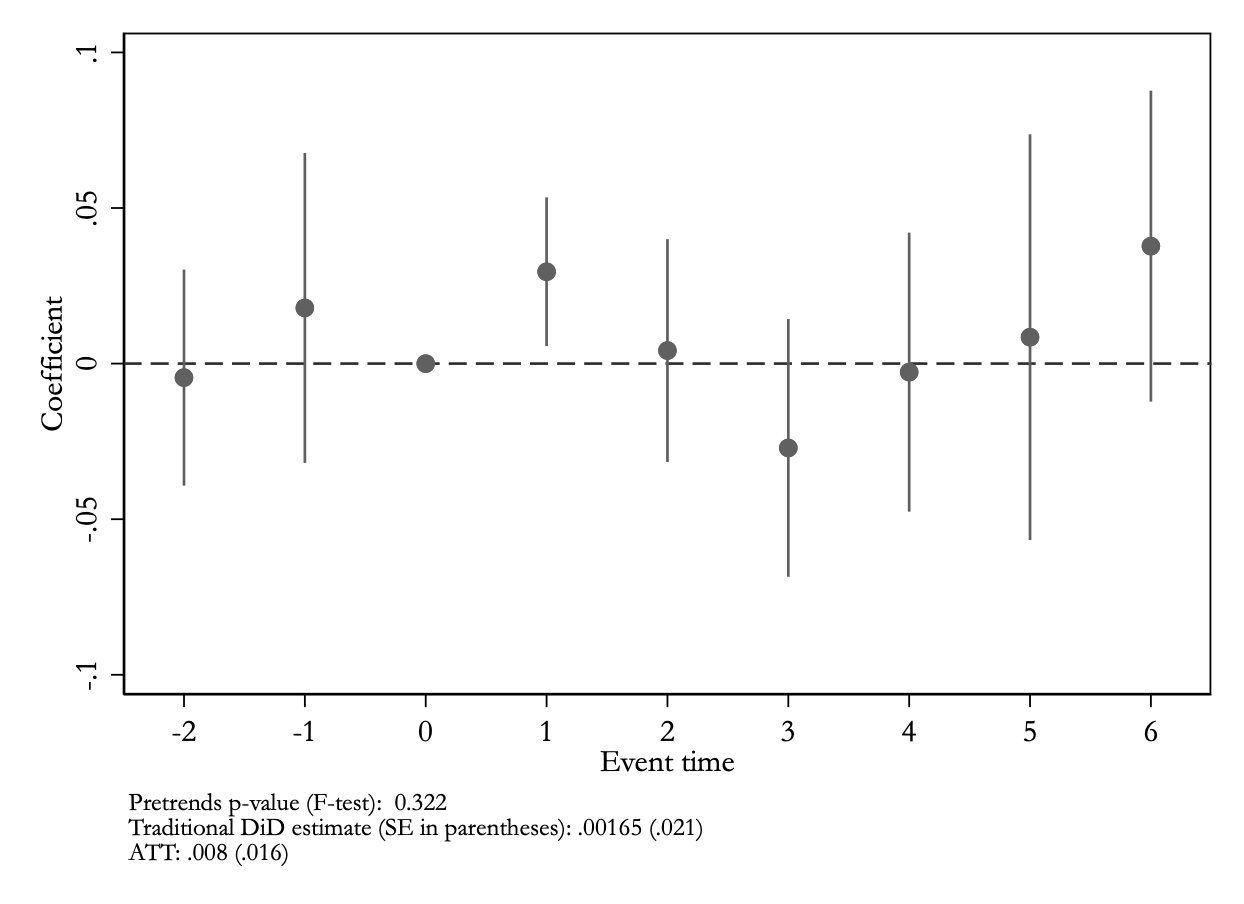
\includegraphics[width=7cm]{eventstudy/high_drug_use/reducedform_jb1986.png} }}%
  \label{fig:rs_es_1986}%
\end{figure}

\begin{footnotesize}
  \noindent Note: These figures report coefficients from the estimation of equation 1 evaluating the impact of the Anti-Drug Abuse Act of 1986 on college enrollment rates using CPS-UCR merged data from 1984-1992. Figure A defines high-intensity states using Black adult arrests, while Figure B defines high-intensity states using Black juvenile arrests. Event time $0 \coloneqq 1986$. The coefficients represent the change in outcomes for high black adult drug arrest states relative to non-high-drug arrest states, where high-drug arrest states are defined to be those above the 75th percentile in 1984. The sample is defined as black males aged 18-24 in 1986 who were not incarcerated at the time of the survey. Control variables include population and unemployment rates at the state-year level. 
\end{footnotesize}

\clearpage

\begin{figure}[h]
  \centering
  \caption{Effect of Fair Sentencing Act on the College Enrollment Rate of Adult Black Men, Comparing High and Low-Intensity States}%
  \subfloat[\centering Using adults arrests]{{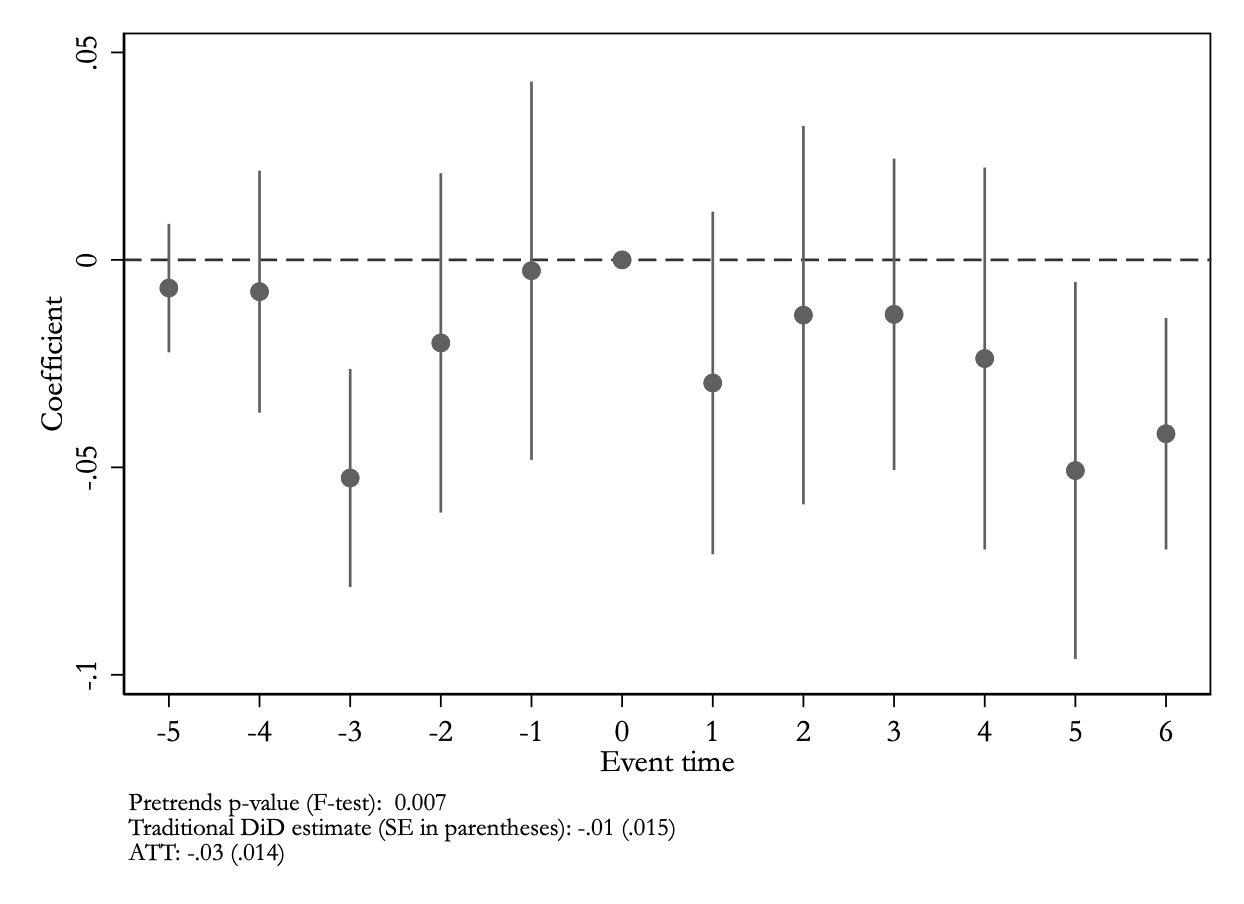
\includegraphics[width=7cm]{eventstudy/high_drug_use/reducedform_ab2010.png} }}%
  \qquad
  \subfloat[\centering Using juvenile arrests]{{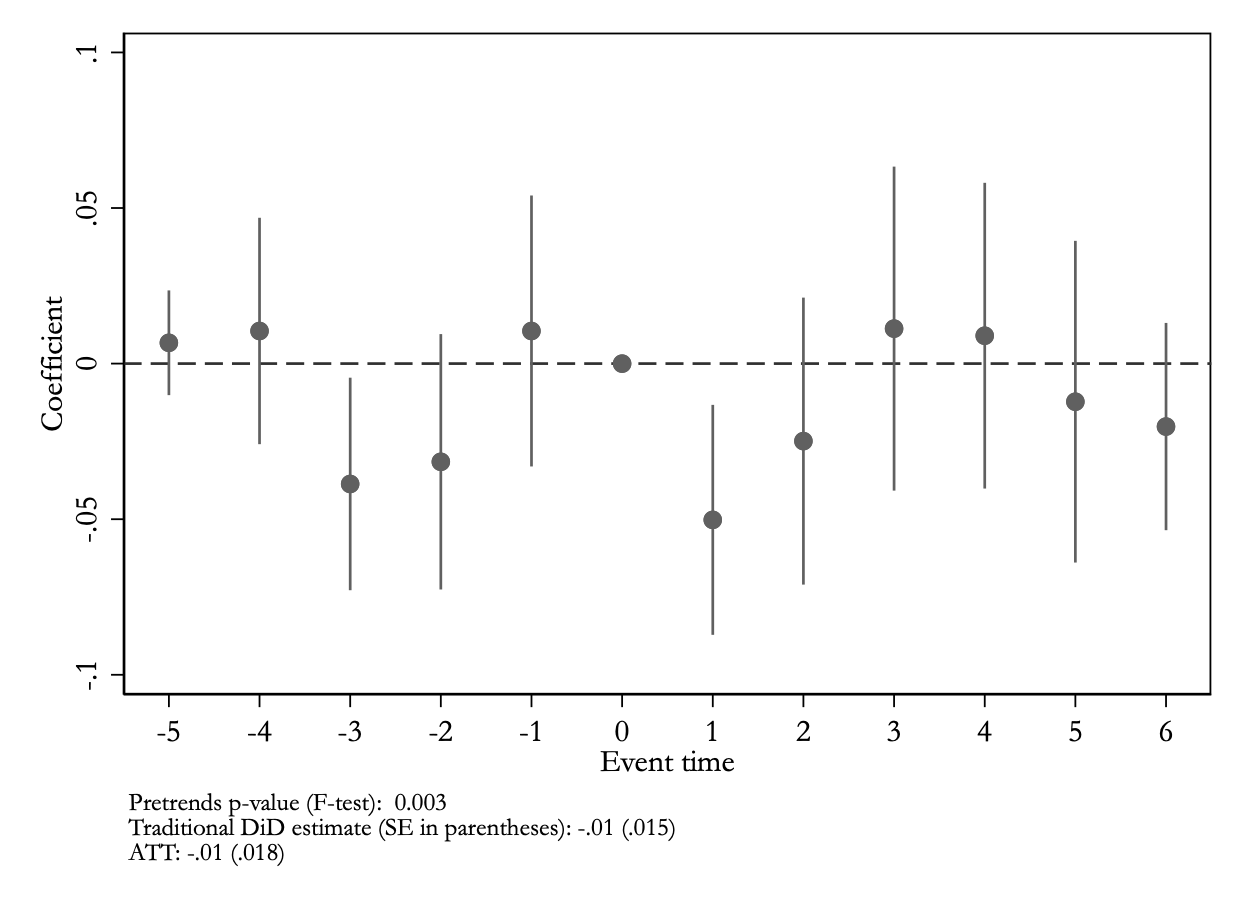
\includegraphics[width=7cm]{eventstudy/high_drug_use/reducedform_jb2010.png} }}%
  \label{fig:rf_jb_es_2010}%
\end{figure}

\begin{footnotesize}
  \noindent Note: These figures report coefficients from the estimation of equation 1 evaluating the impact of the Fair Sentencing Act of 2010 on college enrollment rates using CPS-UCR merged data from 2005-2015. Figure A defines high-intensity states using Black adult arrests, while Figure B defines high-intensity states using Black juvenile arrests. Event time $0 \coloneqq 2010$. The coefficients represent the change in outcomes for high black adult drug arrest states relative to non-high-drug arrest states, where high-drug arrest states are defined to be those above the 75th percentile in 2008. The sample is defined as black males aged 18-24 in 2010 who were not incarcerated at the time of the survey. Control variables include population and unemployment rates at the state-year level. 
\end{footnotesize}

\clearpage


%%%%%%%%%%%%%%%%%%%%%%%%TABLES%%%%%%%%%%%%%%%%%%%%%%%%%%%
\clearpage


\import{../../output/tables/summ_stats/}{cps_ucr_summ_stats.tex}

\begin{footnotesize}
  \noindent Note: Sample means with education supplement weights are calculated from the CPS-UCR merged dataset from 1984 to 1992 and 2000 to 2016. The sample in columns 1 and 2 is defined as persons aged 18-24 in 1986, and the sample in columns 3 and 4 is defined as persons aged 18-24 in 2010, both of whom were not incarcerated at the time of the survey.
\end{footnotesize}

\clearpage

\import{../../output/tables/ddiv}{ddiv_show2.tex}
\begin{footnotesize}
  \noindent Note: The CPS-UCR merged dataset is used for this table.  Mean estimates are weighted using CPS October supplement weights. No controls or fixed effects were used, and significance stars are omitted. Robust standard errors are clustered at the state level. The sample is defined as males aged 18-24 in 1986 who were not incarcerated at the time of the survey. 
\end{footnotesize}

\clearpage

\import{../../output/tables/ddiv}{iv.tex}
\begin{footnotesize}
  \noindent Note: The CPS-UCR merged dataset is used for this table. Estimates are weighted using CPS October supplement weights. The controls used at the individual level include age, age-squared, Latino ethnicity, and binned family income. The controls used at the state level include unemployment and population.
  Robust standard errors are clustered at the state level. The sample is defined as males aged 18-24 in 1986 who were not incarcerated at the time of the survey. 
\end{footnotesize}

\clearpage

%DiD High/low intensity 

\import{../../output/tables/}{DiD_1986_high_low.tex}
\begin{footnotesize}
  \noindent Note: Estimates are weighted using CPS October supplement weights. Robust standard errors are clustered at the state level. The controls used include age, age-squared, Latino ethnicity, yearly state average unemployment rates, and (binned) family income. The sample is defined as males aged 18-24 in 1986 who were not incarcerated at the time of the survey.
\end{footnotesize}

\import{../../output/tables/}{DiD_1986_high_low_cont.tex}
\begin{footnotesize}
  \noindent Note: Estimates are weighted using CPS October supplement weights. Robust standard errors are clustered at the state level. Controls: age, age-squared, Latino ethnicity, yearly state average unemployment rates, and (binned) family income. The sample is defined as males aged 18-24 in 1986 who were not incarcerated at the time of the survey.
\end{footnotesize}
\clearpage

\import{../../output/tables/}{DiD_1986_high_low_jb.tex}
\begin{footnotesize}
  \noindent Note: Estimates are weighted using CPS October supplement weights. Robust standard errors are clustered at the state level. The controls used include age, age-squared, Latino ethnicity, yearly state average unemployment rates, and (binned) family income. The sample is defined as males aged 18-24 in 1986 who were not incarcerated at the time of the survey.
\end{footnotesize}

\import{../../output/tables/}{DiD_1986_high_low_jb_cont.tex}
\clearpage

\import{../../output/tables/}{DiD_1986_high_low_jb_cont_control_experiment_female.tex}


\import{../../output/tables/}{DiD_1986_high_low_jb_cont_control_experiment_old.tex}

\clearpage

\import{../../output/tables/}{DiD_2010_high_low.tex}
\begin{footnotesize}
  \noindent Note: Treated observations are defined as those living in states with a high-drug arrest rate for black adults, where high black adult drug arrest states are defined to be those above the 75th percentile in 2008. Estimates are weighted using CPS October supplement weights. Robust standard errors are clustered at the state level. Controls: age, age-squared, Latino ethnicity, yearly state average unemployment rates, and (binned) family income. The sample is defined as males aged 18-24 in 1986 who were not incarcerated at the time of the survey.
\end{footnotesize}

\import{../../output/tables/}{DiD_2010_high_low_cont.tex}
\begin{footnotesize}
  \noindent Note: Treatment is continuous. Estimates are weighted using CPS October supplement weights. Robust standard errors are clustered at the state level. Controls: age, age-squared, Latino ethnicity, yearly state average unemployment rates, and (binned) family income. The sample is defined as males aged 18-24 in 2010 who were not incarcerated at the time of the survey.
\end{footnotesize}
\clearpage

% Britton Table 2
\import{../../output/tables/}{britton_table2_DiD.tex}
\begin{footnotesize}
  \noindent Note: Estimates are weighted using CPS October supplement weights. Robust standard errors are clustered at the state level. The controls used include age, age-squared, Latino ethnicity, and binned family income. The sample is defined as Black and White males aged 18-24 in 1986 who were not incarcerated at the time of the survey.
  This table is partially replicated from \cite{britton2022}.
\end{footnotesize}

\import{../../output/tables/}{britton_table3_DiD.tex}
\begin{footnotesize}
  \noindent Note: Estimates are weighted using CPS October supplement weights. Robust standard errors are clustered at the state level. The controls used include age, age-squared, Latino ethnicity, and binned family income. The sample is defined as Black males and Black females aged 18-24 in 1986 who were not incarcerated at the time of the survey. This table is partially replicated from \cite{britton2022}.
\end{footnotesize}

\clearpage

\import{../../output/tables/}{britton_table2_DiD_control_experiment.tex}
\begin{footnotesize}
  \noindent Note: Estimates are weighted using CPS October supplement weights. Robust standard errors are clustered at the state level. The controls used include age, age-squared, Latino ethnicity, and binned family income. The sample is defined as Black and White males aged 30-50 in 1986 who were not incarcerated at the time of the survey.
  This table is a control experiment for table 2 in \cite{britton2022}.
\end{footnotesize}

\import{../../output/tables/}{britton_table3_DiD_control_experiment.tex}
\begin{footnotesize}
  \noindent Note: Estimates are weighted using CPS October supplement weights. Robust standard errors are clustered at the state level. The controls used include age, age-squared, Latino ethnicity, and binned family income. The sample is defined as Black males and Black females aged 30-50 in 1986 who were not incarcerated at the time of the survey.
  This table is a control experiment for table 3 in \cite{britton2022}.
\end{footnotesize}
\clearpage

\import{../../output/tables/}{fair_sentencing_DiD_t1.tex}
\begin{footnotesize}
  \noindent Note: Estimates are weighted using CPS October supplement weights. Robust standard errors are clustered at the state level. The controls used include age, age-squared, Latino ethnicity, and binned family income. The sample is defined as Black and White males aged 18-24 in 2010 who were not incarcerated at the time of the survey.
\end{footnotesize}

\import{../../output/tables/}{fair_sentencing_DiD_t2.tex}
\begin{footnotesize}
  \noindent Note: Estimates are weighted using CPS October supplement weights. Robust standard errors are clustered at the state level. The controls used include age, age-squared, Latino ethnicity, and binned family income. The sample is defined as Black males and females aged 18-24 in 2010 who were not incarcerated at the time of the survey.
\end{footnotesize}

\import{../../output/tables/}{fair_sentencing_DiD_t1_control_experiment.tex}
\begin{footnotesize}
  \noindent Note: Estimates are weighted using CPS October supplement weights. Robust standard errors are clustered at the state level. The controls used include age, age-squared, Latino ethnicity, and binned family income. The sample is defined as Black and White males aged 30-50 in 2010 who were not incarcerated at the time of the survey.
\end{footnotesize}

\import{../../output/tables/}{fair_sentencing_DiD_t2_control_experiment.tex}
\begin{footnotesize}
  \noindent Note: Estimates are weighted using CPS October supplement weights. Robust standard errors are clustered at the state level. The controls used include age, age-squared, Latino ethnicity, and binned family income. The sample is defined as Black males and females aged 30-50 in 2010 who were not incarcerated at the time of the survey.
\end{footnotesize}
\clearpage

\import{../../output/tables/ddd}{ddd_1986_ab.tex}
\begin{footnotesize}
  \noindent Note: CPS data from 1984-1992.
  The sample is defined as males aged 18-24 in 1986 who were not incarcerated at the time of the survey.
\end{footnotesize}

\clearpage

\import{../../output/tables/ddd}{ddd_1986_jb.tex}

\clearpage

\import{../../output/tables/ddd}{ddd_2010_ab.tex}

\clearpage

\import{../../output/tables/ddd}{ddd_2010_jb.tex}
\clearpage 


%%%%%%%%%%%%%%%%%%%%%%%%APPENDIX%%%%%%%%%%%%%%%%%%%%%%%%%%%
\clearpage

\begin{appendices}
  \section{Data}
  I include a summary statistics table for the CPS data that is not merged with the UCR program data.

  \section{Additional Results}
  The contents...
  \section{First stage arrest rate estimates}
  I include tables for the equation \ref{eq:state_level_es} estimates presented in figures XYZ.


  In \cite{britton2022}, when examining the impact of the Anti-Drug Abuse Act of 1986, she commences her analysis in 1984 due to "fluctuations in Black college enrollment during the early 1980s that were unrelated to the emergence of drug markets \cite{nces}".

 

  \section{Reduced form college enrollment estimates}
  I include tables for the equation \ref{eq:state_level_es} estimates presented in figures XYZ.


  \clearpage

  % Appendix figures
  
% 1986 pretrends

\begin{figure}[h]
    \centering
    \caption{College Enrollment Around 1984}%
    \subfloat[\centering By race]{{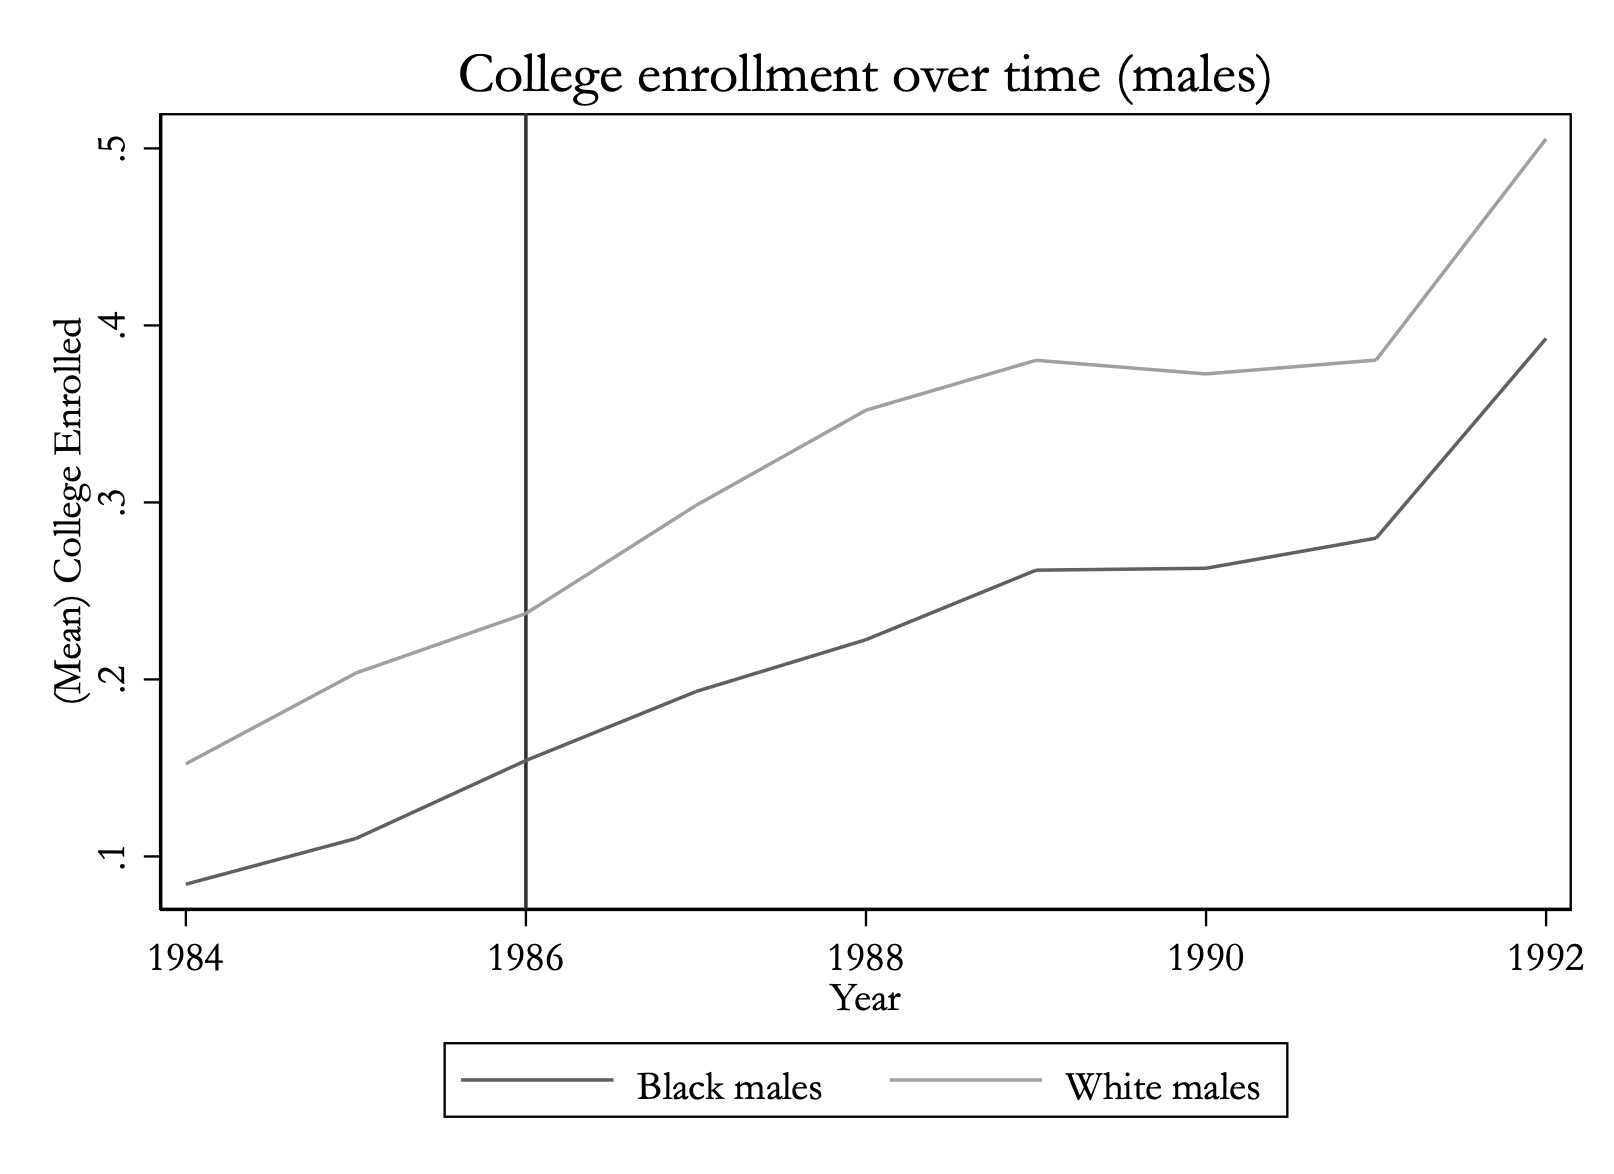
\includegraphics[width=7cm]{pretrends/1986/college_enroll_byrace_1986.png} }}%
    \qquad
    \subfloat[\centering By sex]{{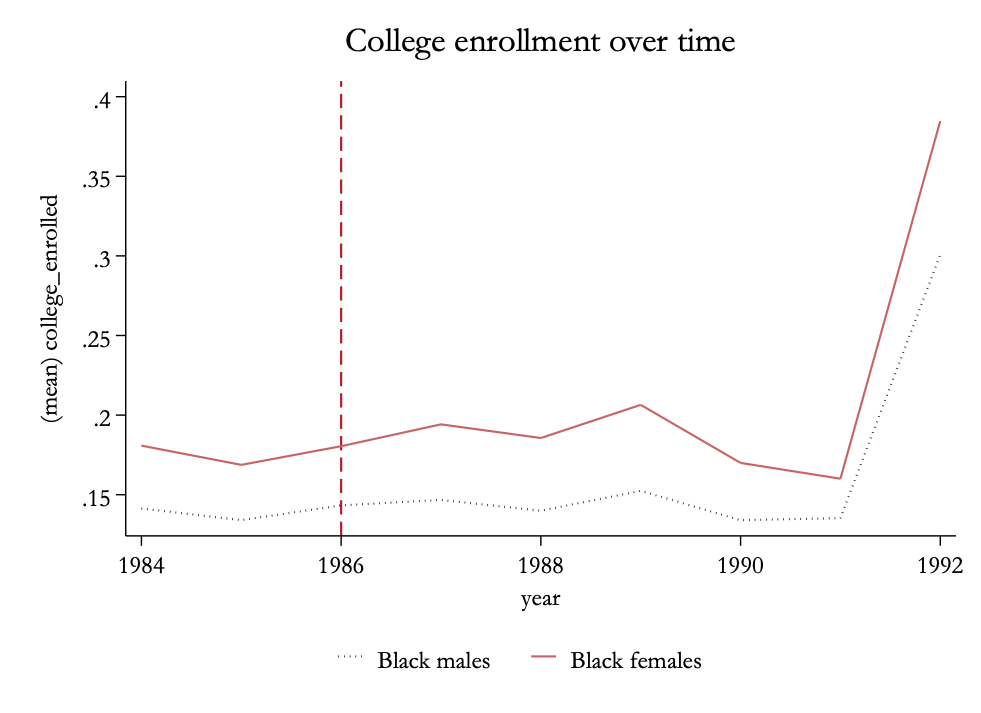
\includegraphics[width=7cm]{pretrends/1986/college_enroll_bysex_1986.png} }}%
    \label{fig:raw_college_1986}%
  \end{figure}
  
  \begin{figure}[h]
    \centering
    \caption{Family Income Around 1984}%
    \subfloat[\centering By race]{{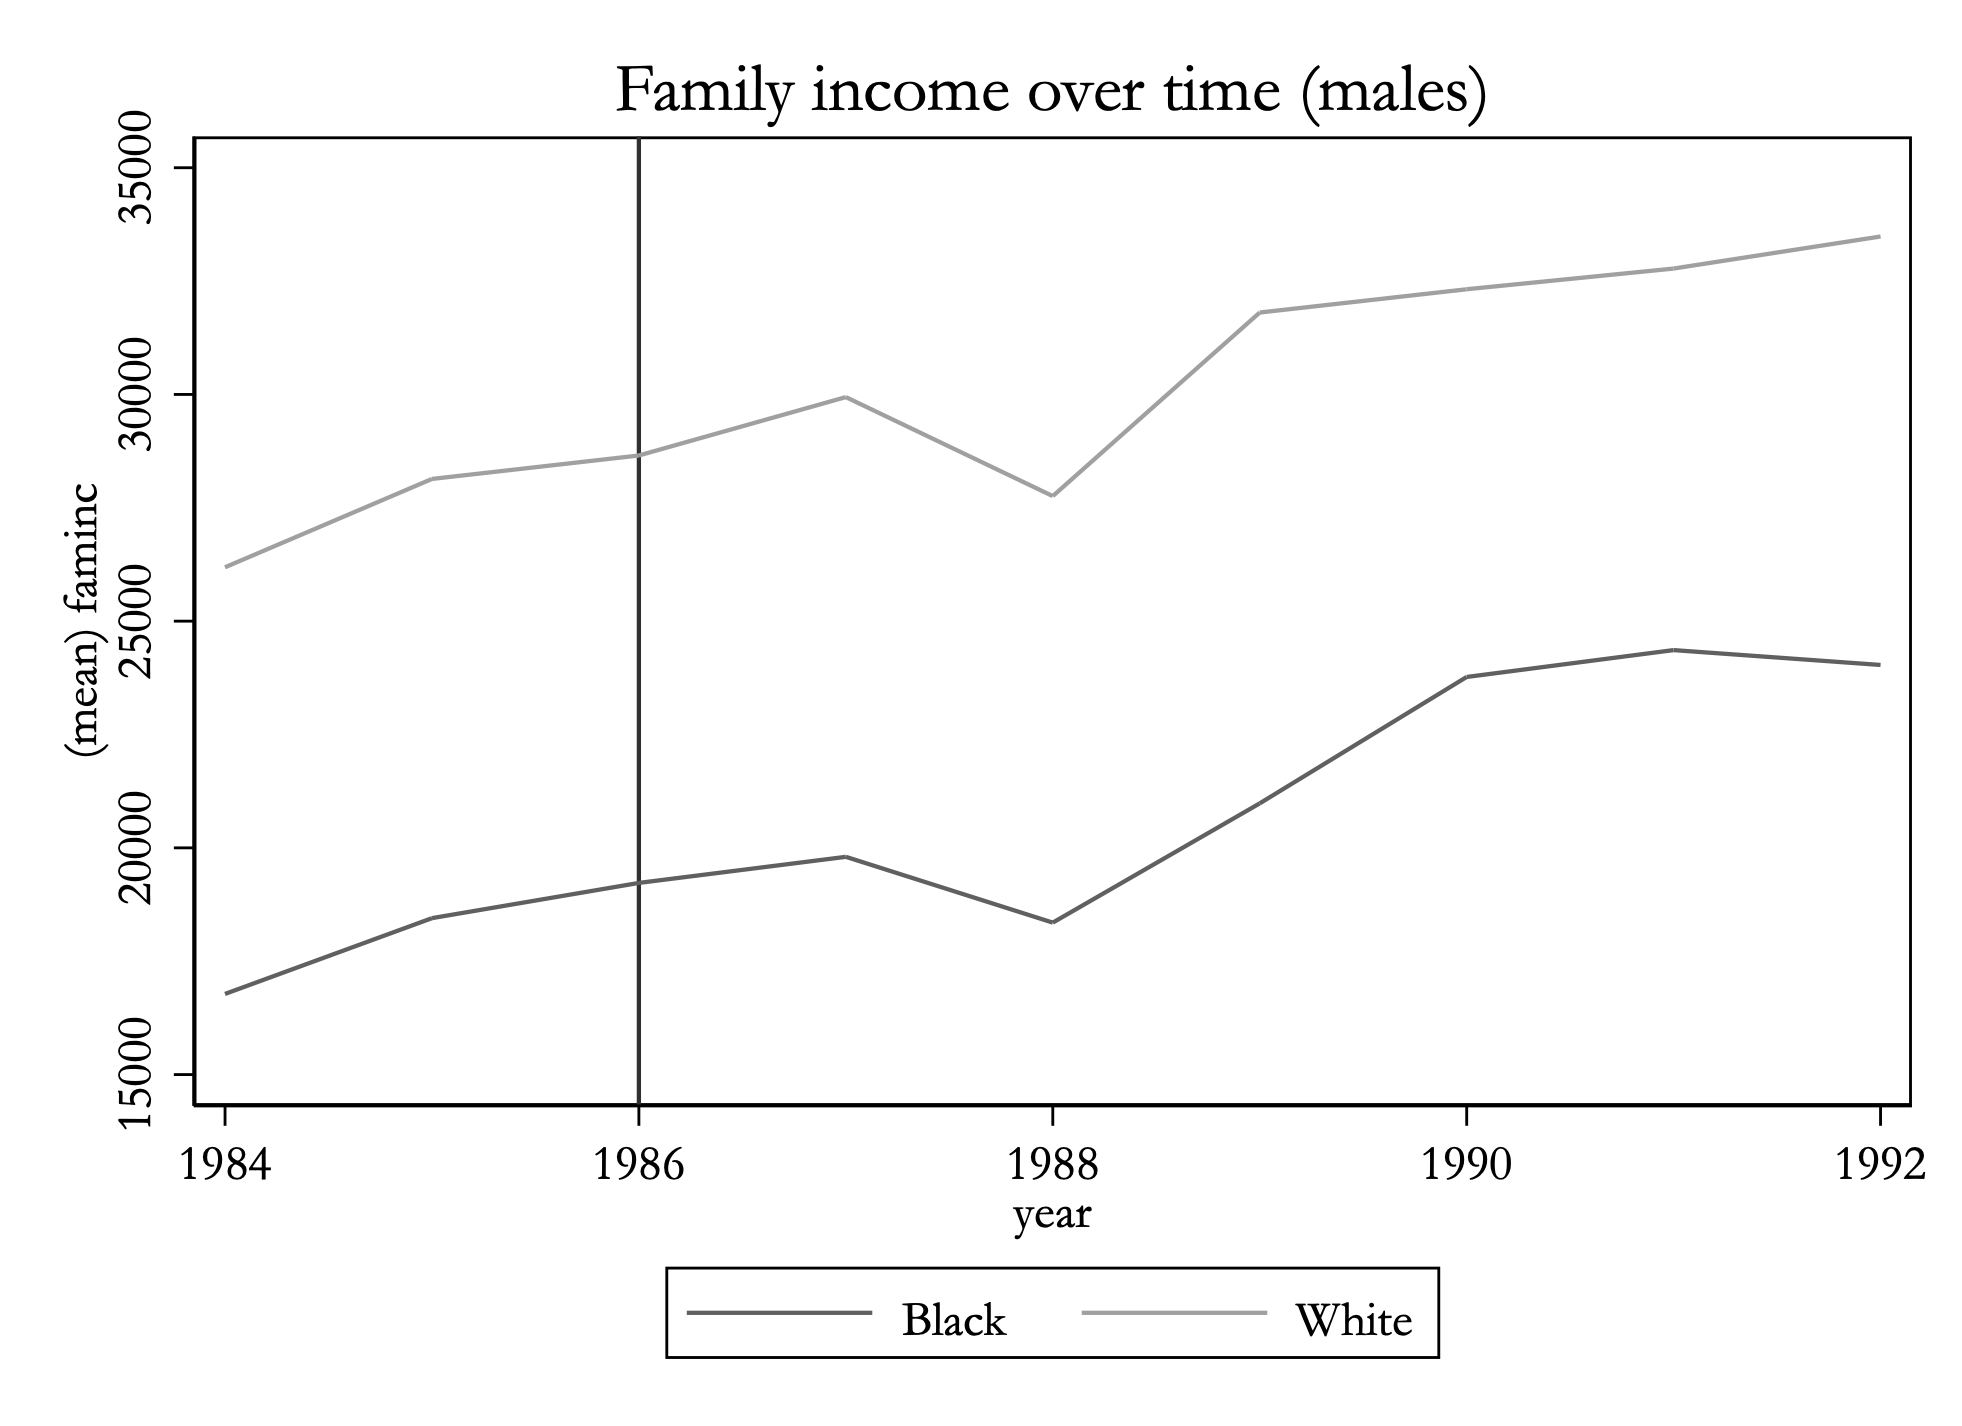
\includegraphics[width=7cm]{pretrends/1986/faminc_byrace_1986.png} }}%
    \qquad
    \subfloat[\centering By sex]{{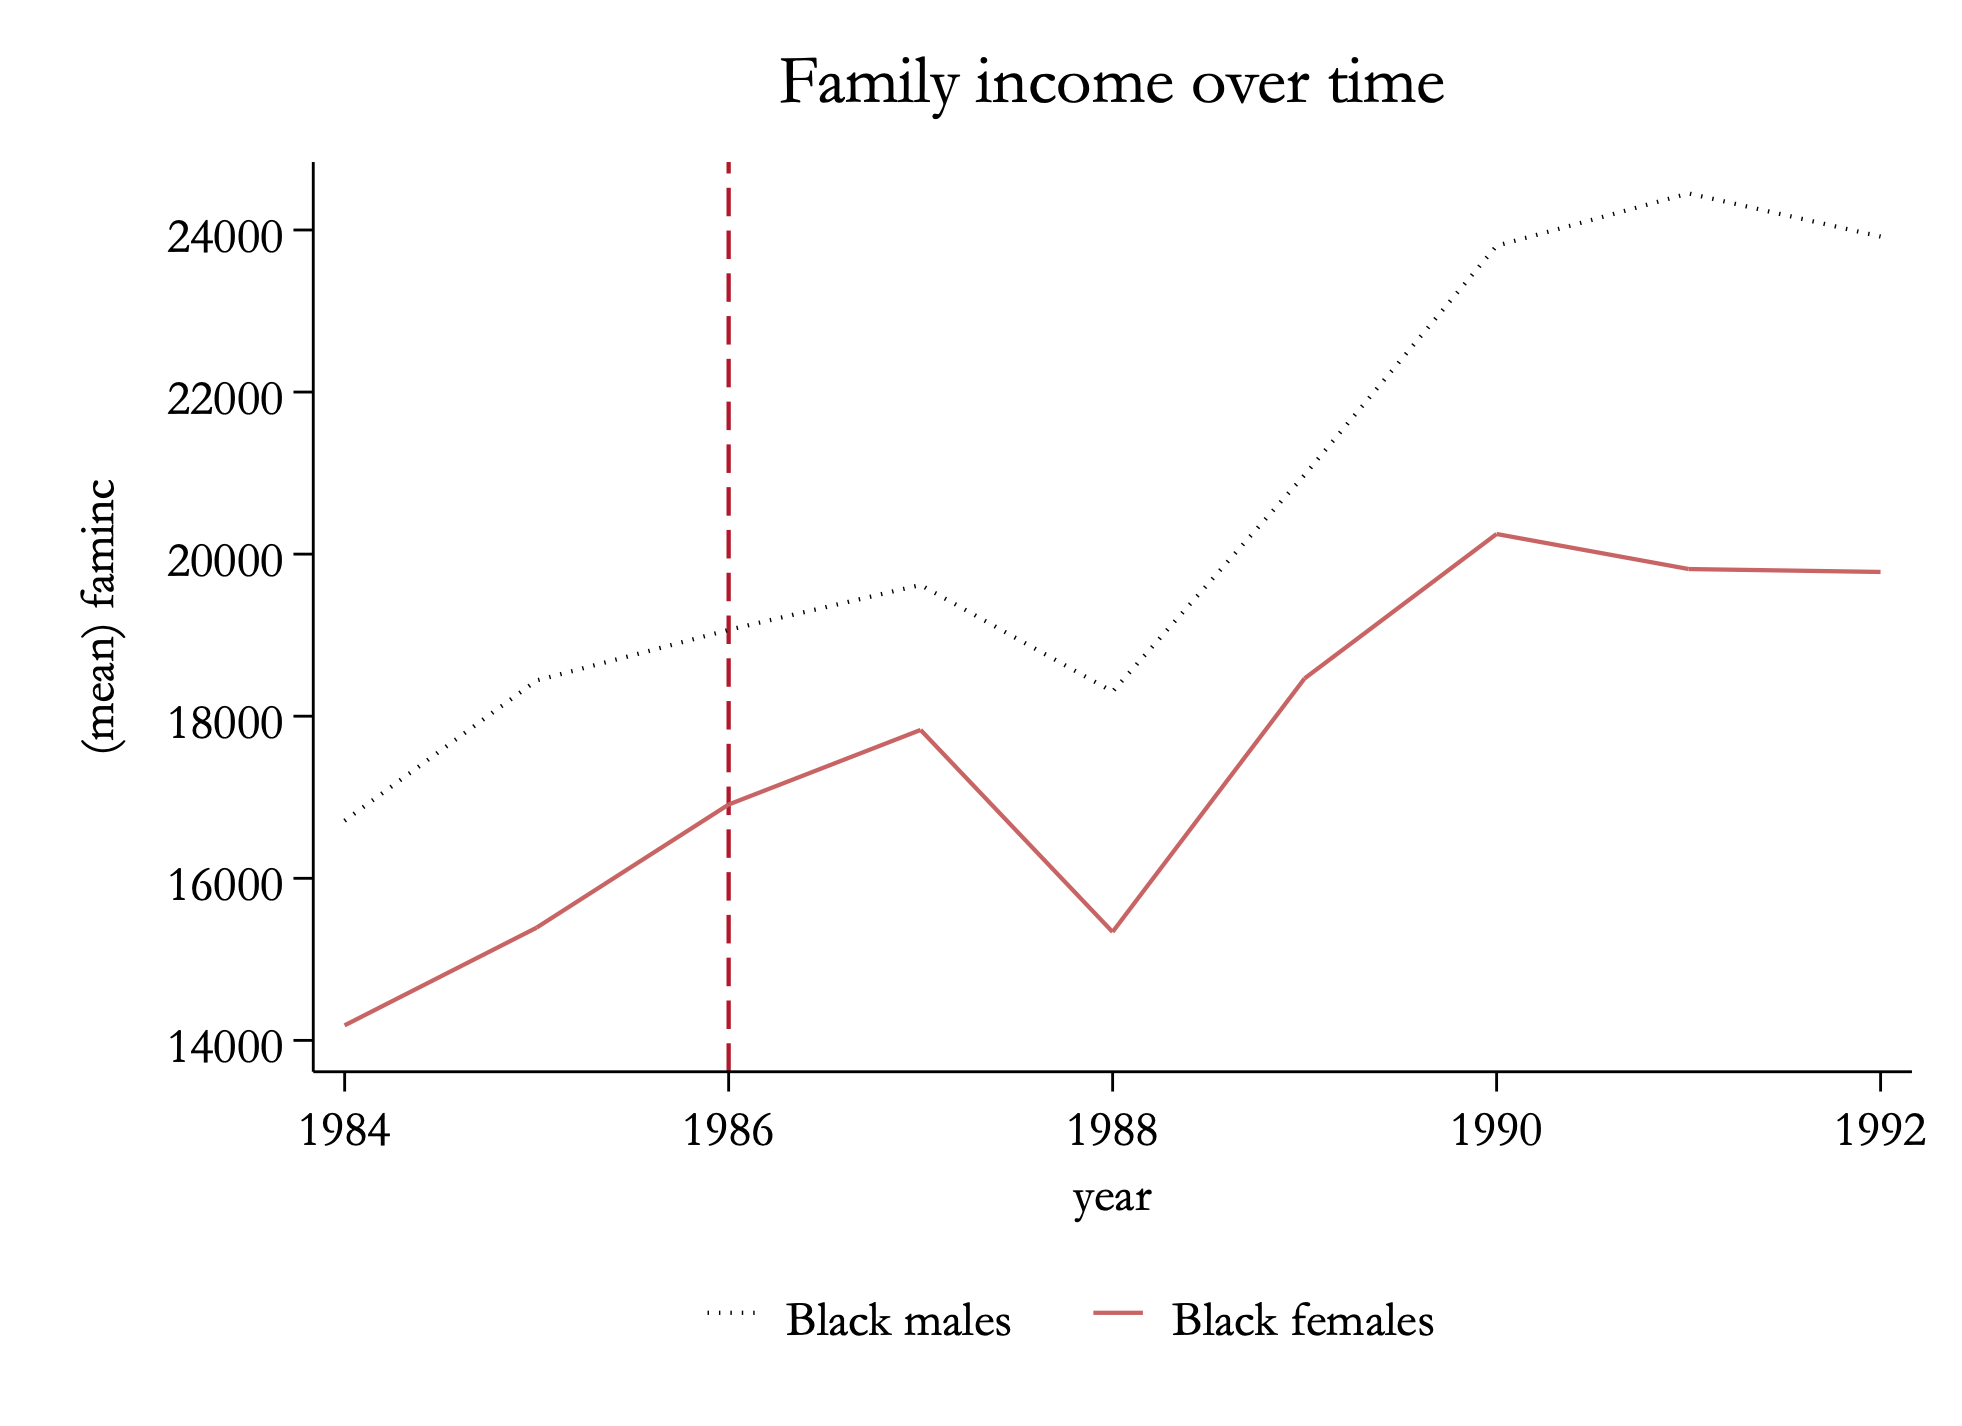
\includegraphics[width=7cm]{pretrends/1986/faminc_bysex_1986.png} }}%
    \label{fig:raw_faminc_1986}%
  \end{figure}
  
  \begin{footnotesize}
    \noindent Note: These figures report the outcomes for various subgroups plotted over time using CPS data from 1984-1992. Figure \ref{fig:raw_college_1986} reports the proportion enrolled in college, while figure \ref{fig:raw_faminc_1986} reports the average family income. A vertical line is drawn to denote the passage of the Anti-Drug Abuse Act of 1986. The universe of samples is defined as participants aged 18-24 in 1986 who were not incarcerated at the time of the survey.
  \end{footnotesize}
  
  \clearpage
  
  % 2010 pretrends
  
  \begin{figure}[h]
    \centering
    \caption{College Enrollment Around 2010}%
    \subfloat[\centering By race]{{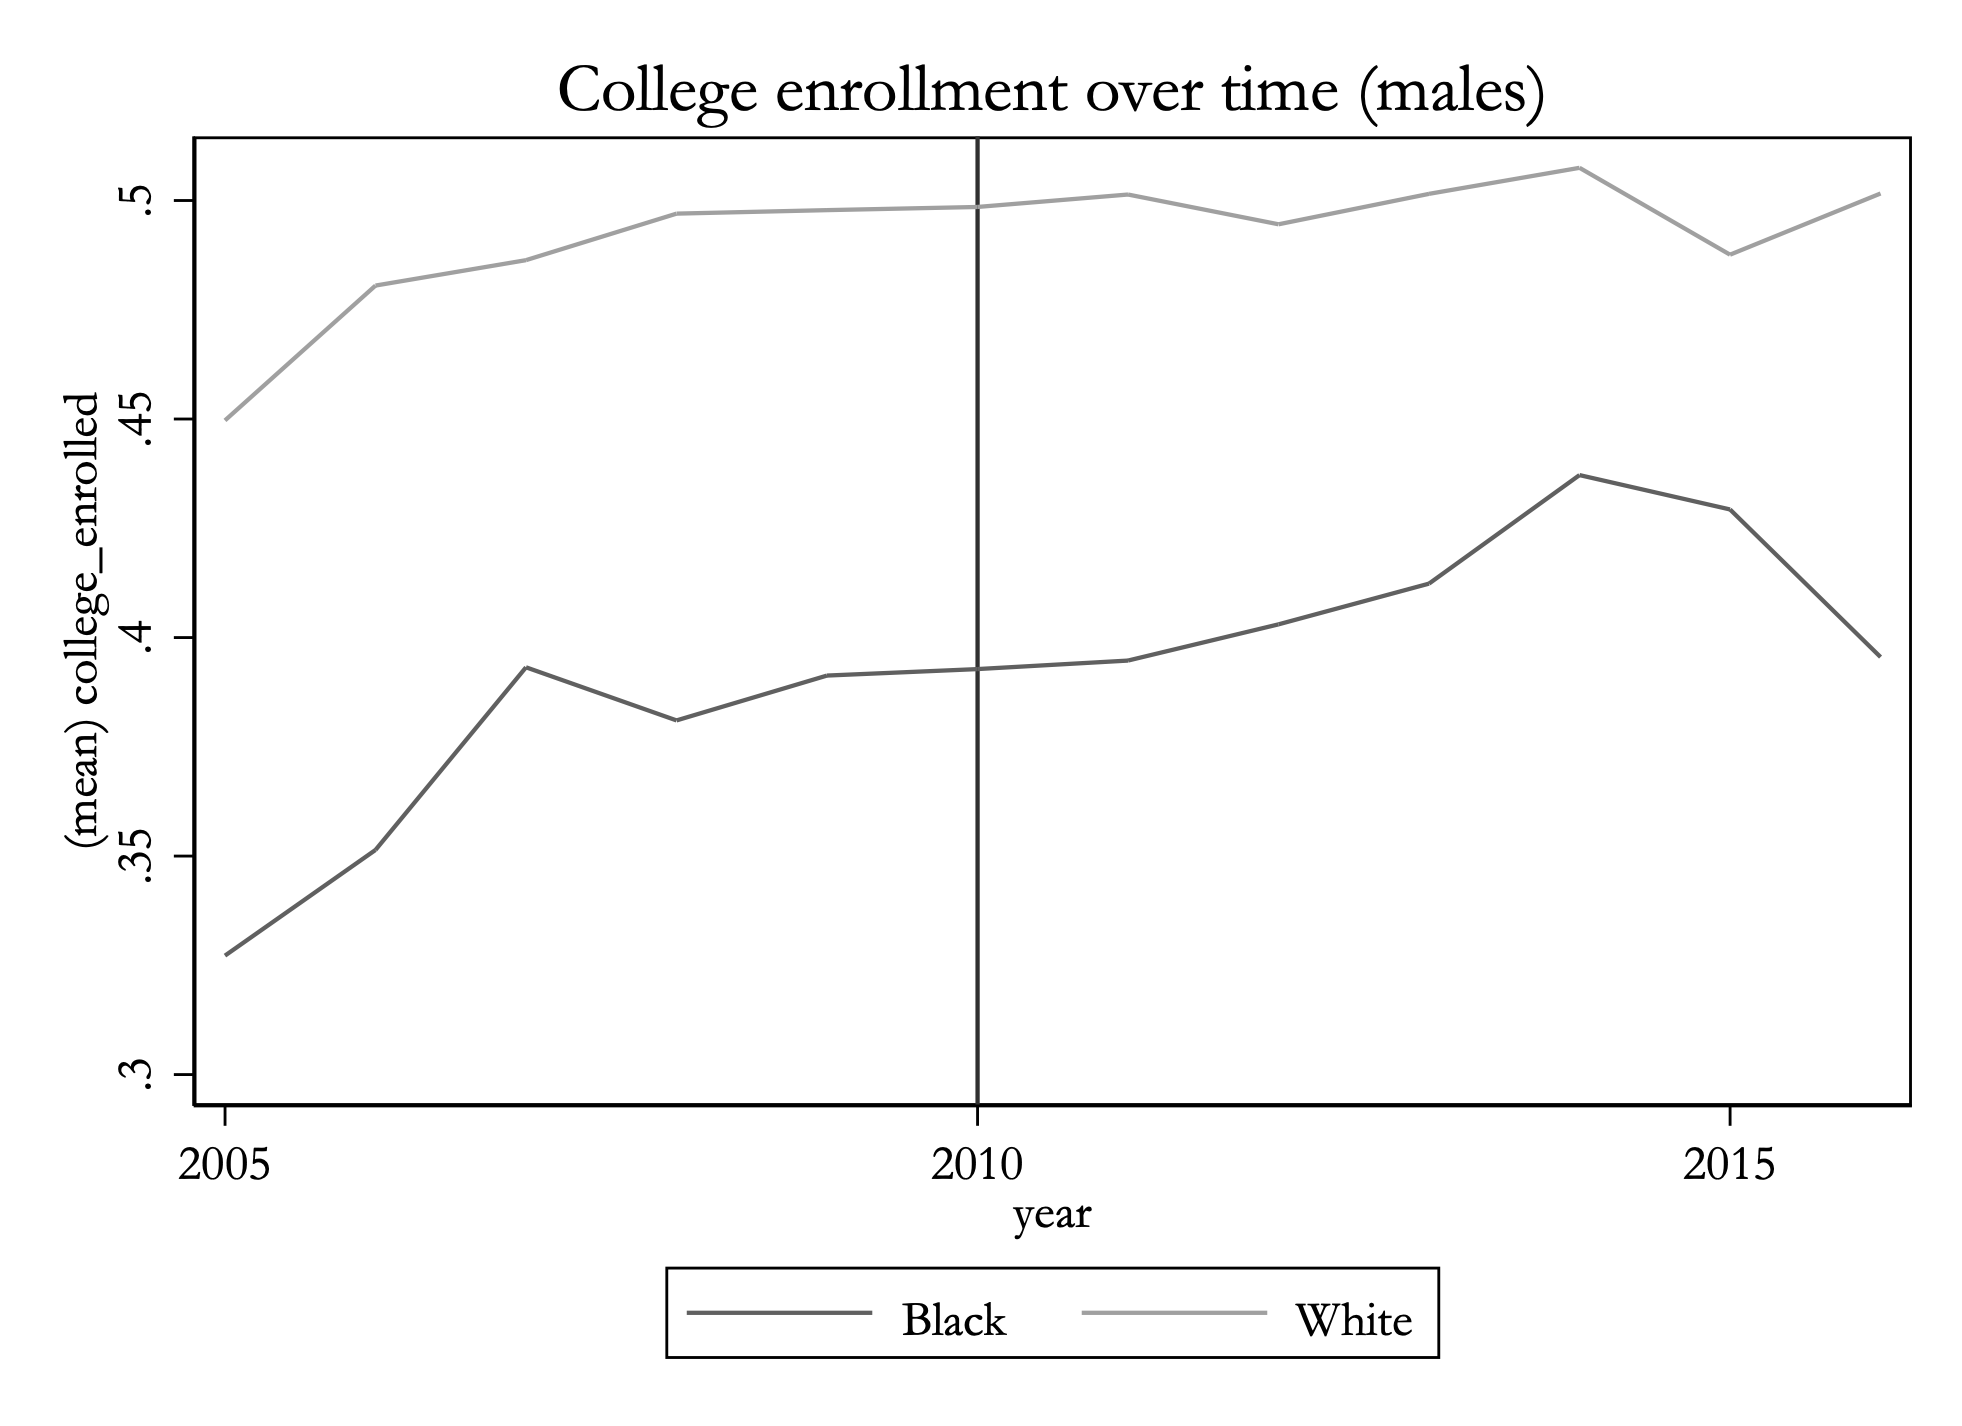
\includegraphics[width=7cm]{pretrends/2010/college_enroll_byrace_2010.png} }}%
    \qquad
    \subfloat[\centering By sex]{{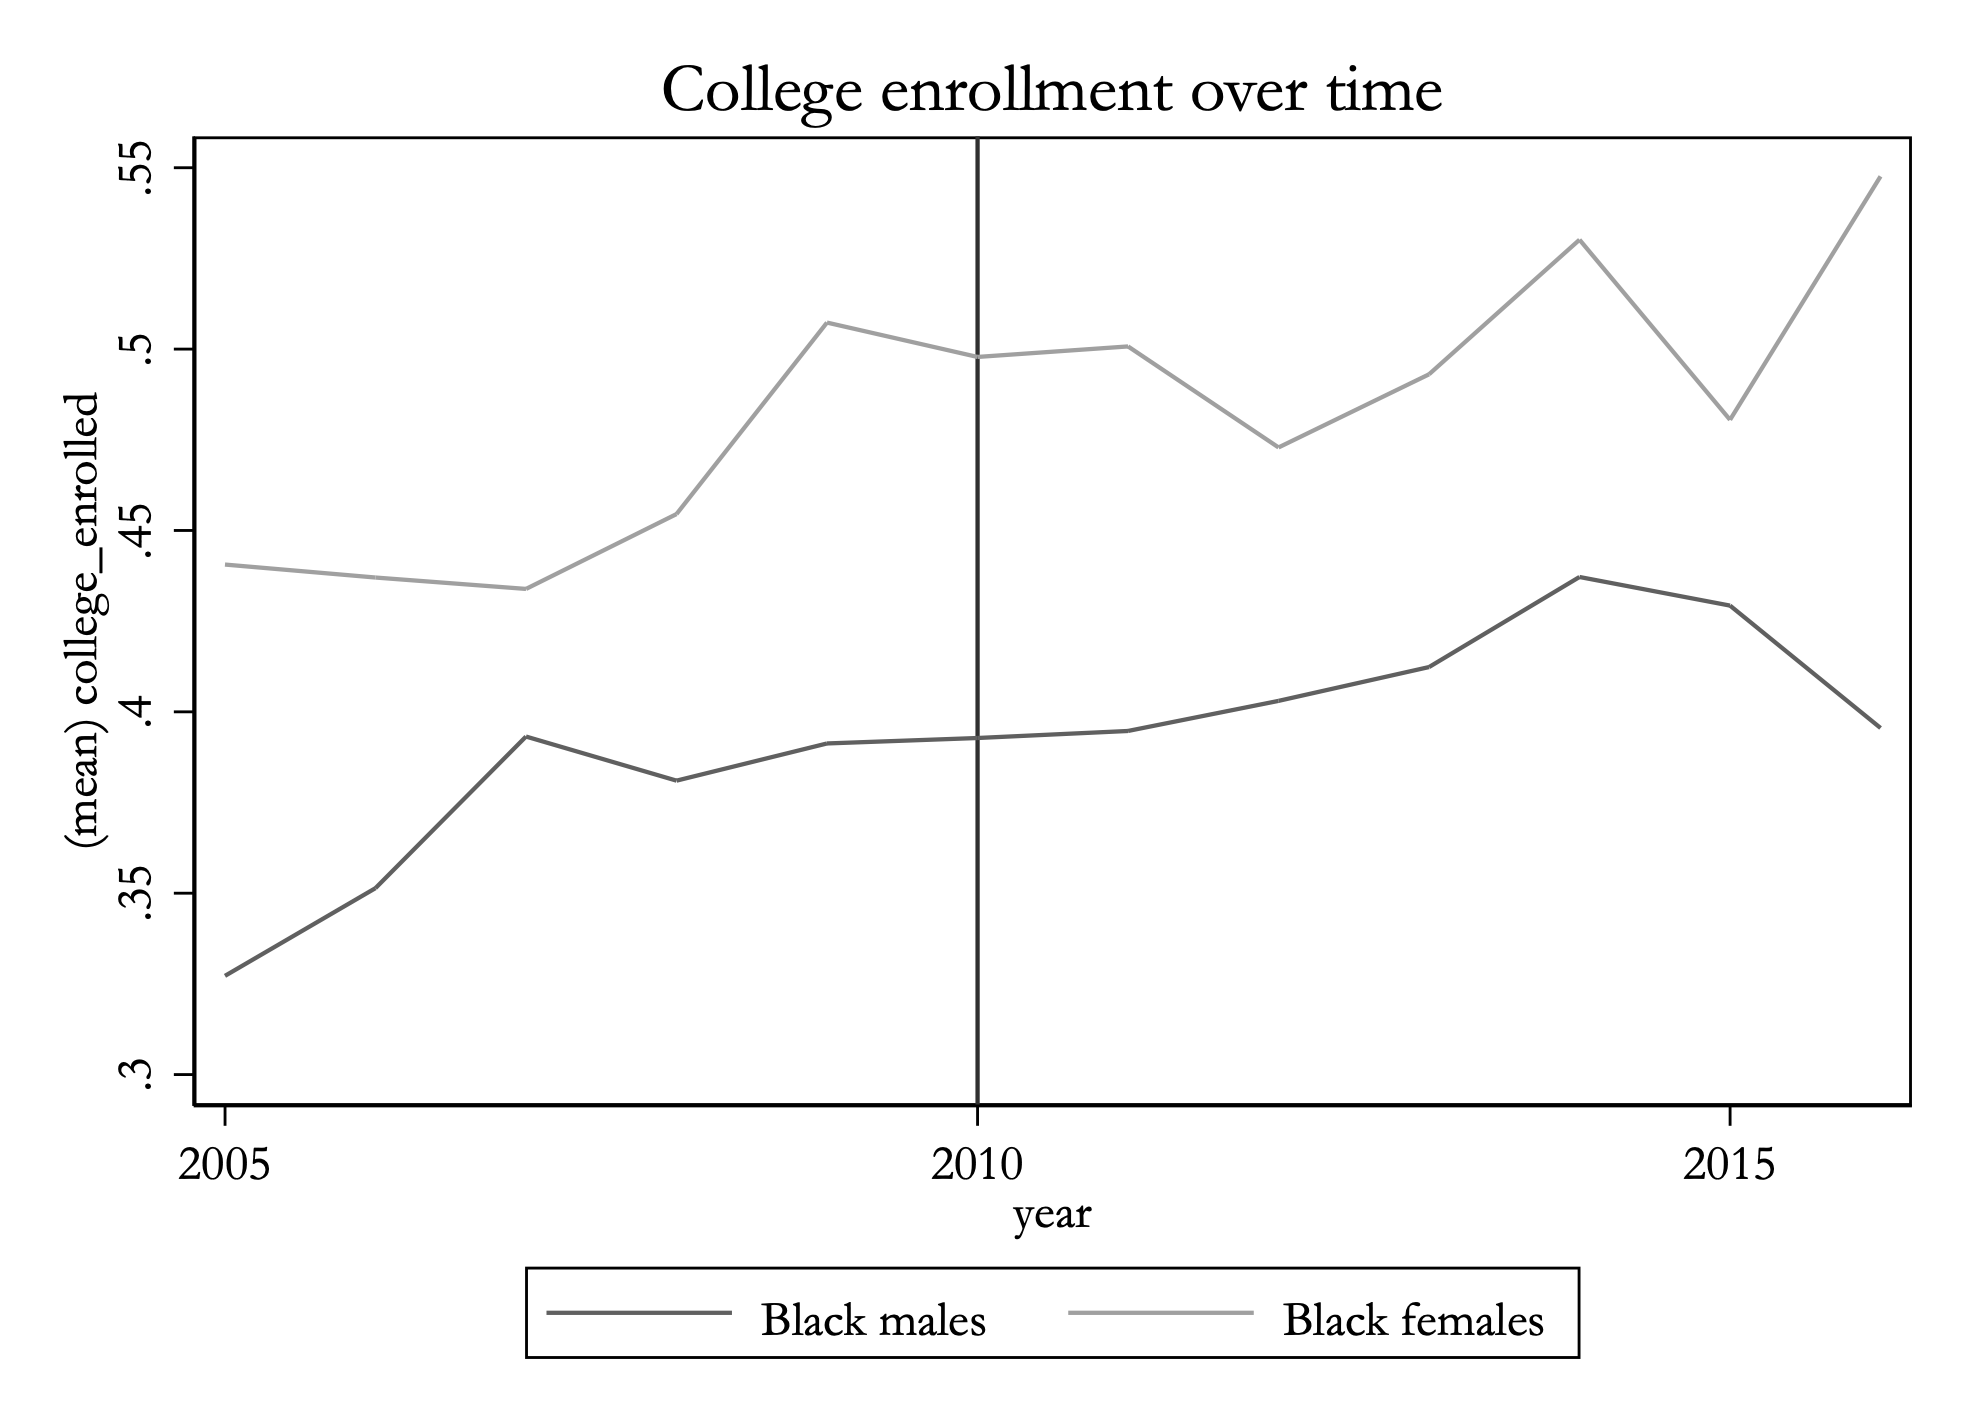
\includegraphics[width=7cm]{pretrends/2010/college_enroll_bysex_2010.png} }}%
    \label{fig:raw_college_2010}%
  \end{figure}
  
  \begin{figure}[h]
    \centering
    \caption{Family Income Around 2010}%
    \subfloat[\centering By race]{{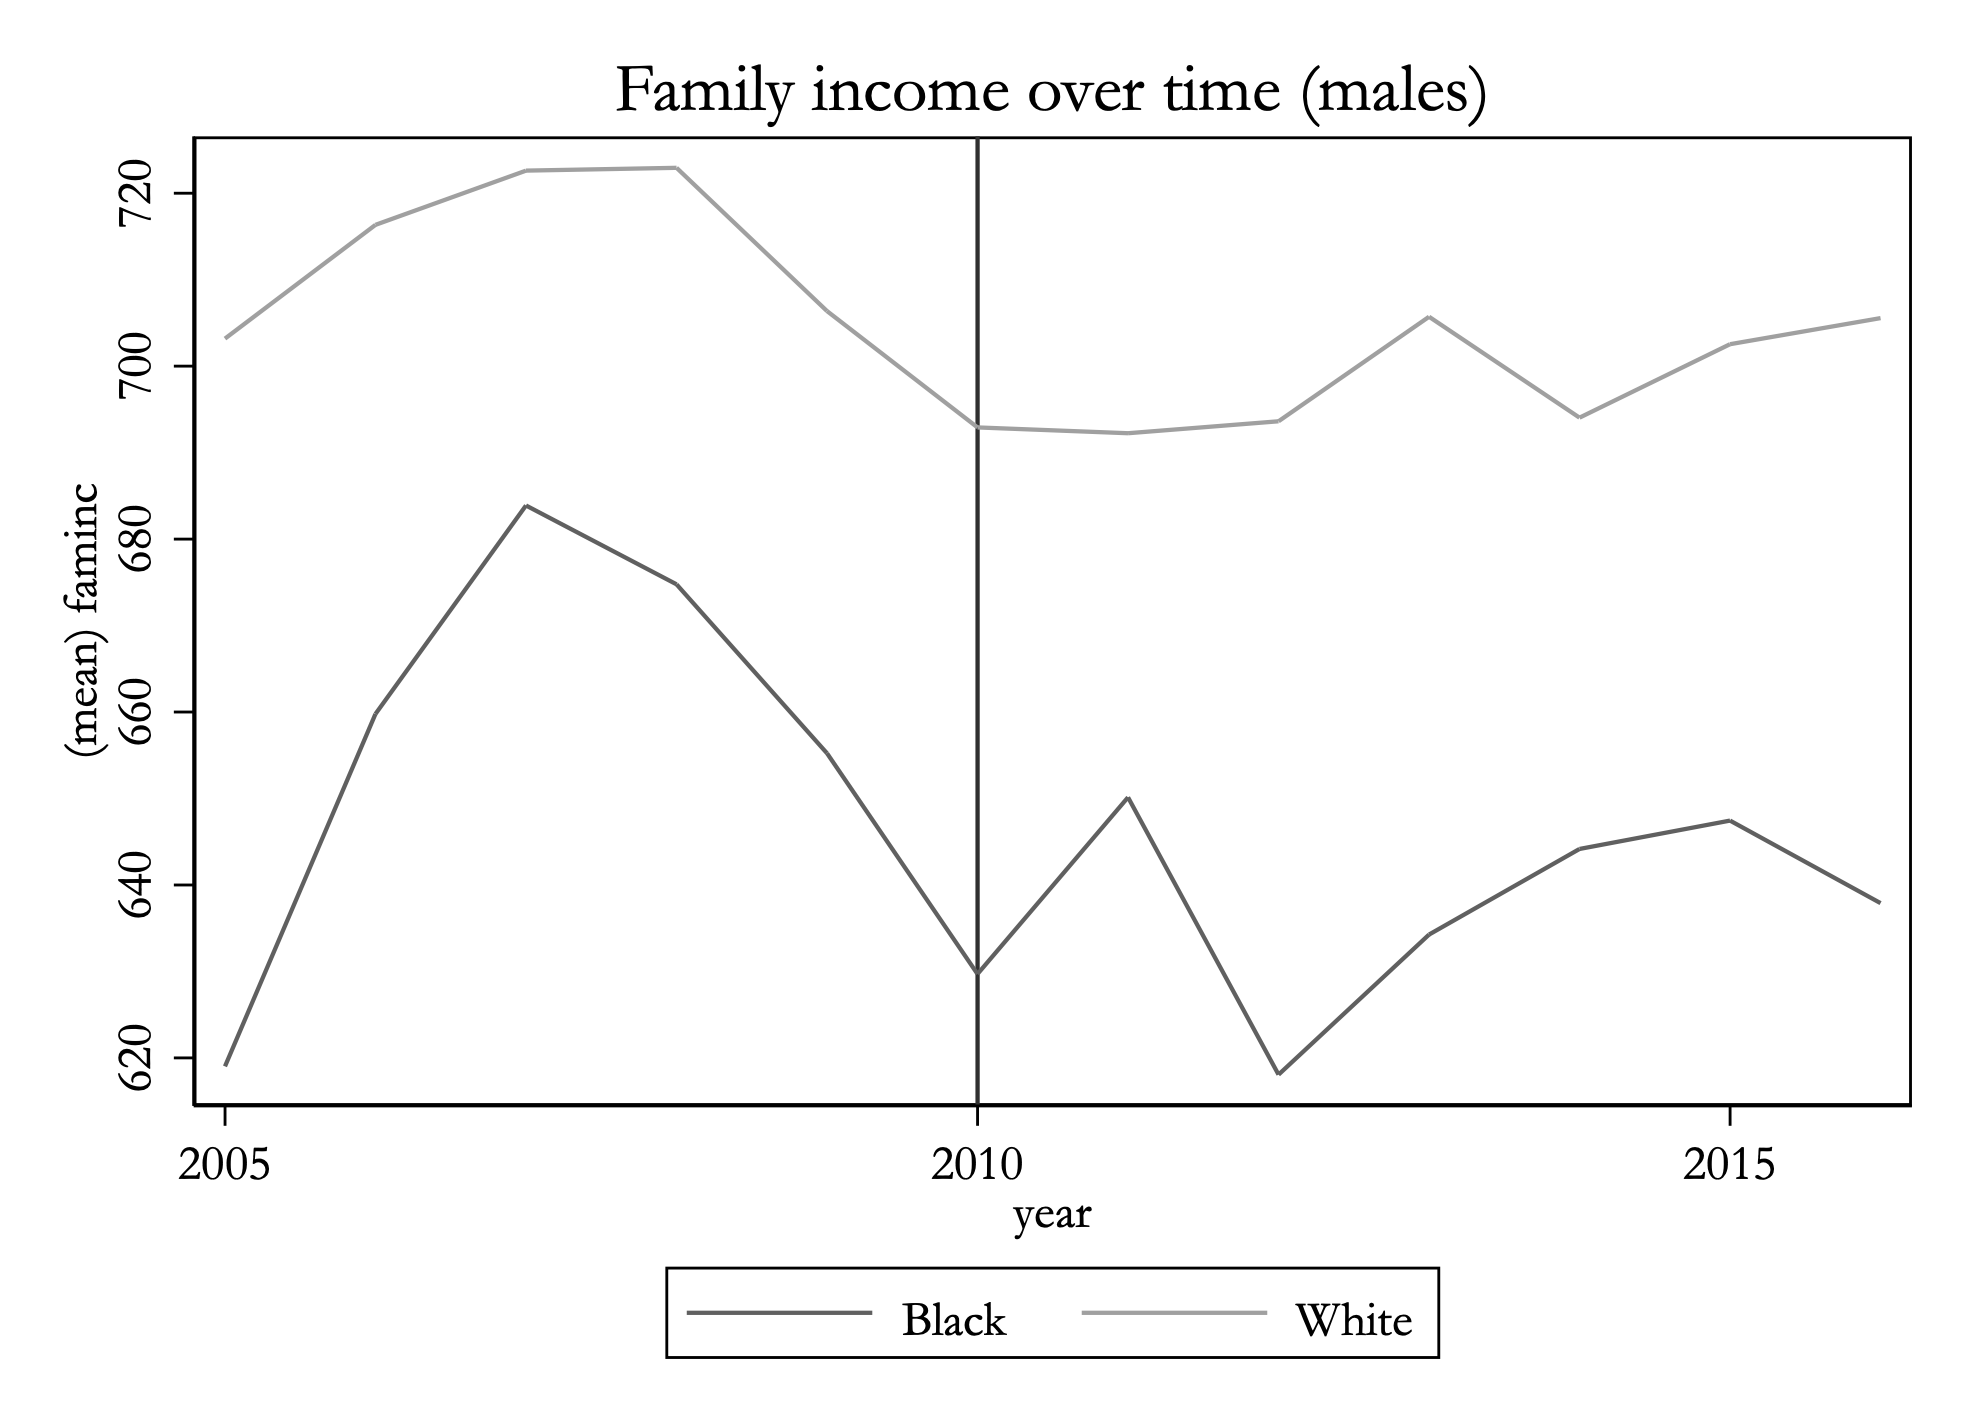
\includegraphics[width=7cm]{pretrends/2010/faminc_byrace_2010.png} }}%
    \qquad
    \subfloat[\centering By sex]{{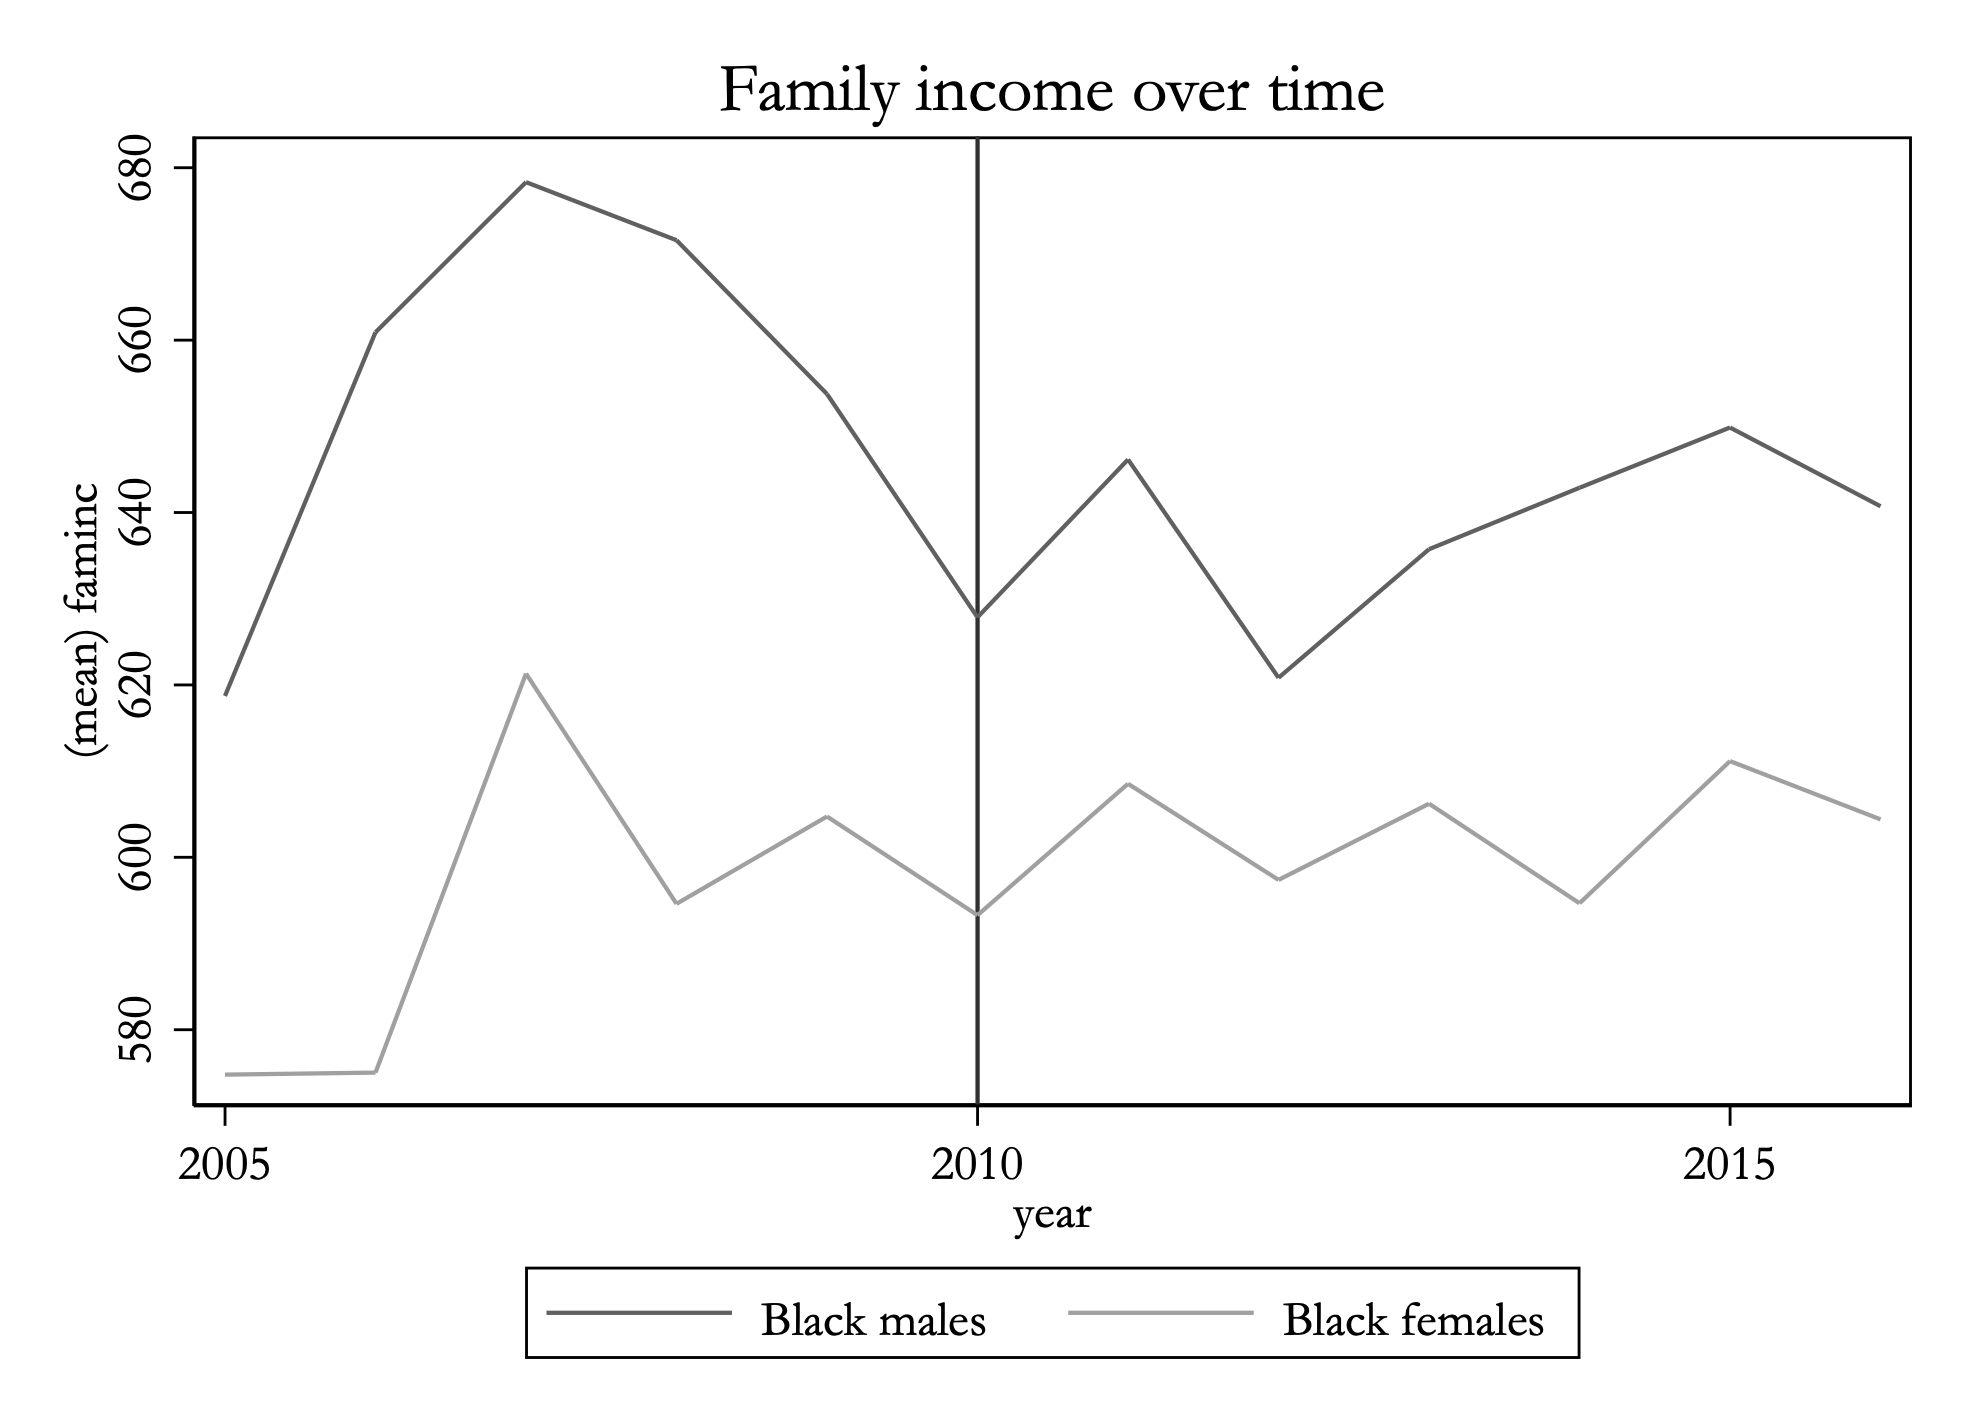
\includegraphics[width=7cm]{pretrends/2010/faminc_bysex_2010.png} }}%
    \label{fig:raw_faminc_2010}%
  \end{figure}
  
  \begin{footnotesize}
    \noindent Note: These figures report the outcomes for various subgroups plotted over time using CPS data from 2005-2016. Figure \ref{fig:raw_college_2010} reports the proportion enrolled in college, while figure \ref{fig:raw_faminc_2010} reports the average family income. A vertical line is drawn to denote the passage of the Fair Sentencing Act of 2010. The universe of samples is defined as participants aged 18-24 in 2010 who were not incarcerated at the time of the survey.
  \end{footnotesize}

  \clearpage

  \begin{figure}[h]
    \caption{Effect of Anti-Drug Abuse Act on Drug-related Arrest Rate of Adult Black Men, Comparing States with High and Low Black Adult Drug-Related Arrest Rates}
    \centering
    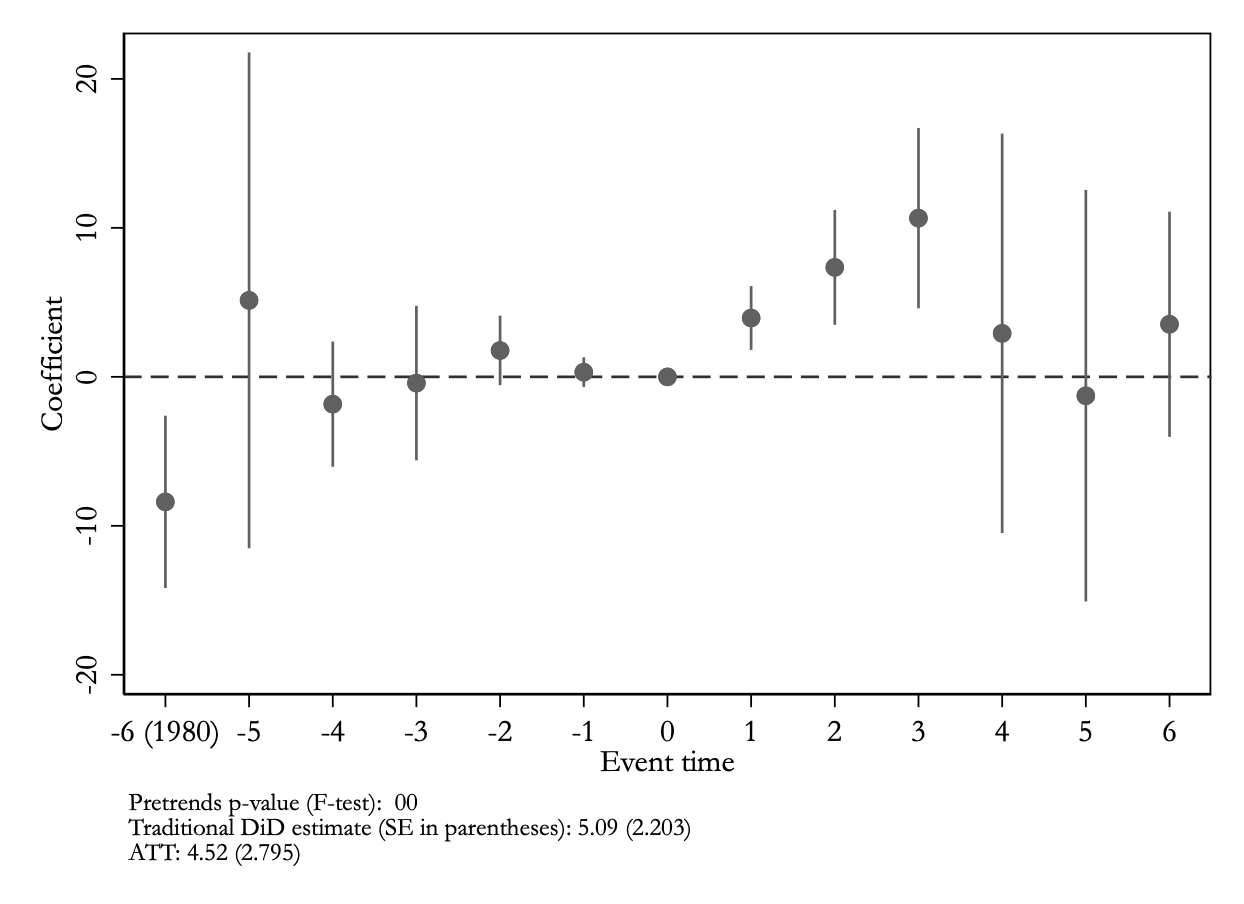
\includegraphics[width=1\textwidth]{eventstudy/high_drug_use/high_drug_eventstudy_1986_extended_years.png}
    \label{fig:b1}
  \end{figure}
  \begin{footnotesize}
    \noindent Note: footnote TO BE UPDATED
  \end{footnotesize}


  
  \clearpage

  % Appendix tables
  \import{../../output/tables/summ_stats/}{cps_only_summ_stats.tex}
  \begin{footnotesize}
    \noindent Note: Sample means with education supplement weights are calculated from the CPS October supplement dataset from 1984 to 1992 and 2000 to 2016. The sample in columns 1 and 2 is defined as persons aged 18-24 in 1986, and the sample in columns 3 and 4 is defined as persons aged 18-24 in 2010, both of whom were not incarcerated at the time of the survey. This table is partially replicated from \cite{britton2022}.
  \end{footnotesize}
  \clearpage
  % First stage event study table
  \import{../../output/tables/eventstudy}{eventstudy_firststage.tex}

  \clearpage

  % Reduced form
  \import{../../output/tables/eventstudy}{eventstudy_reducedform.tex}


\end{appendices}



\end{document}
